\documentclass[12pt,a4paper,twocolumn]{article}
\usepackage[utf8]{inputenc}
\usepackage[T1]{fontenc}
\usepackage[british]{babel}
\usepackage{indentfirst} 
\usepackage{graphicx}
\usepackage{tabularx}
\usepackage{siunitx}
\usepackage{amsmath,stix,bm}
%% fur amsmath, comment garamond and add
%% 'stix' btwn amsmath and bm
\usepackage{eucal}
%\usepackage{amsfonts}
%\usepackage{amssymb}
%\usepackage{wasysym}
%\usepackage{booktabs}
\usepackage{caption}
%\usepackage{lmodern}
\usepackage{multicol}
\usepackage[includeheadfoot,margin=0.35in,bottom=0.7in]{geometry}
%%\usepackage{avant}
%Per grafica vettoriale tramite InkScape%
\usepackage{color}
\usepackage{transparent}
\graphicspath{{img/}}
\usepackage[dvipsnames]{xcolor}
\usepackage{pdfpages}
\usepackage{pgfplots}
\usepackage{textcomp}
\usepackage{tgbonum}
\usepackage{xcolor,colortbl}
%\usepackage{simpsons}
%\usepackage{addfont}
%\addfont[1.5]{OT1}{simfon}{\simfon}
\usepackage{listings}
\usepackage{cleveref}

\usepackage{caption}
\DeclareCaptionFont{quack}{\fontfamily{lmss}\selectfont}
\captionsetup{font={color=gray,quack},labelfont={color=black,bf}}
\usepackage{subcaption}
\usepackage{titlesec}
\titleformat*{\section}{\Large\bfseries\fontfamily{qag}\selectfont\color{Turquoise}}
\titleformat*{\subsection}{\large\bfseries\fontfamily{qag}\selectfont\color{Turquoise}}
\titleformat*{\subsubsection}{\itshape\bfseries\fontfamily{qag}\selectfont\color{Turquoise}}


%\fontfamily{qag}\selectfont\color{Turquoise}
%\fontfamily{qag}\selectfont\color{Turquoise}
%\color{Turquoise} 

\definecolor{mintbg}{rgb}{.63,.79,.95}
%% 
%\graphicspath{{figures/}} %Setting the graphicspat%h
%\graphicspath{{figures/}} %Setting the graphicspath
\graphicspath{{figures/}{figures/A/}{figures/B/}} %Setting the graphicspath
\makeatletter
%\providecommand*{\input@path}{}
%\edef\input@path{{figures/}{}\input@path}% prepend
\def\input@path{{figures/}{figures/A/}{figures/B/}{figures/C/}}
\makeatother
\usepackage{import}

\pgfplotsset{compat=newest}
\pgfplotsset{plot coordinates/math parser=false}
\newlength\figureheight
\newlength\figurewidth
\usepackage{placeins}
\usepackage{float}
\usepackage{blindtext}
\usepackage{authblk}
\renewcommand\Affilfont{\tiny \color{gray}}

\title{\vspace*{20 pt}\fontfamily{qag}\selectfont\color{Turquoise}\huge\textbf{Design of an array of folded patches}\vspace*{10 pt}}
%\author{Blasi Luca\thanks{The first author wants to thank someone.}	, Mastrofini Alessandro, Mucenica Stefan Leonard}
\author[1]{Blasi Luca}
\author[2]{Mastrofini Alessandro}
\author[3]{Mucenica Stefan Leonard}
\affil[2]{email}
\affil[3]{email}

\date{}
\usepackage{fancyhdr}
\pagestyle{fancy}
\fancyhf{}
	\lhead{\small\fontfamily{lmss}\selectfont\color{gray} University of Rome Tor Vergata}
\fancyfoot[C]{\thepage\  of \pageref{LastPage}}
\renewcommand{\headrulewidth}{0.50pt}

%\lhead{Guides and tutorials}
\fancypagestyle{plain}{
	\renewcommand{\headrulewidth}{0.5pt}
	%\setlength{\headheight}{80 pt} 
	\lhead{\small\fontfamily{lmss}\selectfont\color{gray} Wireless Electromagnetic Technologies \\
		Professor: Marrocco Gaetano\\
	University of Rome Tor Vergata\\2022}
	\rhead{
\includegraphics[height=60pt]{logo.png} }
	\fancyfoot{}
}
\usepackage{lastpage}

\usepackage{lipsum}
\usepackage[
backend=bibtex,
style=numeric
]{biblatex} %Imports biblatex package
\addbibresource{mybib.bib} %Import the bibliography file

\begin{document}

	{\fontfamily{lmss}\selectfont


%%% MAIN TITLE %%% 


%%% AUTHORS and PROFESSORS%%% 


%%%

\twocolumn[{
\begin{@twocolumnfalse} 
		\vspace*{10 pt}
	\begingroup
	\let\center\flushleft
	\maketitle

	\let\endcenter\endflushleft
	
	\endgroup
		\vspace*{5 pt}
		
		
	\begin{abstract}
	\textcolor{blue}{\lipsum[1-2]}
	\end{abstract}
	\vspace*{20 pt}
\end{@twocolumnfalse}
}
]




\section*{Introduction}
	\textcolor{blue}{\lipsum[1]}
\section*{Tchebyshev array factor design}

\indent A Tchebyshev array factor will be designed in this part, so that the specific structure of the single element of the array is disregarded for the moment. The array is represented by a linear distribution of five elements ($n_{el}=5$), which are supposed to be uniformly spaced and with a non-uniform amplitude for the feed arrangement, that anyway is going to be symmetrical (starting from the element in the middle, located in the origin of the geometrical axes). Also the "\emph{mean lobe to side lobet ratio}" ($R$) will be one of the input design variables. Thus, the variables of this design part are the \emph{element inter-spacing} ($d_{opt}$, which needs to be optimal such that the beamwidth is minimized), the feed amplitude of the single antenna (each one represented by a $C_i$, with $i\in\{-2,-1,0,1,2\}$, the $i^{th}$ \emph{current coefficient} - these unknowns are actually just three and not five, due to the symmetrical amplitude distribution hyphotesis), the operating \emph{resonant frequency} required for the single antenna ($f$) and some other quantities related to them, such as the \emph{tapering efficiency} ($\eta_T$) and the \emph{beamwidth} ($BW_{fn}$). Moreover, the difference between the beamwidth of the Tchebyshev array (\emph{Uniform Spacing Non Uniform Amplitude} case, shorten $NUA$) and  that of a uniform array having the same number of elements and inter-spacing value but a uniform amplitude feed distribution  (\emph{Uniform Spacing Uniform Amplitude}, shorten $UA$) will be discussed. The input design variables related to the Tchebyshev array factor (i.e. $n_{el}$, $R$ and $f$)are listed in \textbf{\cref{table:input_design_cheb}}. 

\indent 

Starting from the optimal inter-element spacing, it requires some secondary variables in orderer to be evaluated. Firstly, a coefficient ($\gamma$, depending on $R$ and indirectly on the number of array elements) neeeds to be calculated, among with the wavelength in the free space ($\lambda$, as the ratio between the light speed in the free space - $c$ - and the operating frequency $f$). Having those quantities, $d_{opt}$ minimizing the $BW_{fn}$ can be computed by using the \textbf{\cref{eq:test}} group. 

\indent 

The array factor evaluation through the Tchebyshev polynomial comes as the next step. The Tchebyshev polynomial approximation to the second order ($T_2(x)$) is sufficient so the current coefficients can be obtained, remembering that a symmetrical amplitude distribution hypothesis has been made. In this case the current coefficients $C_i\,,\,i\in\{-2,-1,0,1,2\}$ follow the rule $C_i=C_{-i}$, thus their symbolic representation can be simplified as follows: $C_n\,,\,n\in\{0,1,2\}$ (or just $n\,=\,\overline{0,2}$). Since the \emph{Riblet variation} to the \emph{Dolph-Tchebyshev synthesis model} has been used, the variable of $T_2(x)$ becomes $x\,=\,a\,+\,b\cos(u)$ and the formulation for $d_{opt}\,\in\,({\lambda}/{2},\lambda]$ differs from the standard model. The coefficients $a$ and $b$ are related to the maximum value selected in the sub-domain of $T_2(x)$ (the window of visible radiation lobes). This maximum, called for example $x_1$, corresponds to the main lobe in which it can be convertend by evaluating the array factor $|T_2(x_1)|$ (some additional references to the specific formulas that need to be used in order to compute can be found in \textbf{\cite{Balanis1}} and \textbf{\cite{ewa}}). That said, the current coefficients can be extracted from $T_2(x)$ (so by using \textbf{\cref{eq:tcheby poly coeff}}). Resulting uniquely out of a $C_n$ dependence, the tapering efficiency is obtained by using \textbf{\cref{eq:tapering efficiency}}.

\indent 

Next, both non uniform amplitude (Tchebyshev array, $NUA$) and uniform amplitude ($UA$)  cases are compared. The comparison shows how the $BW_{fn}$ in the $UA$ case (i.e $BW_{fn}^{[UA]}$) is narrower than that of $NUA$ case (i.e. $BW_{fn}^{[NUA]}$). This result (see \textbf{\cref{eq:tcheby beamwidth}} and \textbf{\cref{table:tcheby results}}) is generally effective and the comparison has been made to show that this particular design case confirms the general condition. 

\indent 

All the numerical quantities related to the Tchebyshev array design are gathered together in \textbf{\cref{table:tcheby results}}. After these quantities are calculated, some important design considerations can be made about the array efficiency. A Non-Uniform Amplitude Array Factor has been designed by using the Riblet variation of the Dolph-Tchebyshev array synthesis model. Considering the \emph{maximum to minimum feed ratio}: \[r_{\max/\min}\,=\,\frac{C_{\max}}{C_{\min}}\] 
the less $r_{\max/\min}$ is, the more efficient distribution of current is reached. In this particular design, the requirement was to to find the $d_{opt}$ which minimizes the beamwidth, starting from the input design variables. Thus, the $r_{\max/\min}$ is a straight consequence of the current coefficients and its optimal value has not been the seek of this project. Anyway, for this design, $r_{\max/\min}\,\cong\,4.39$ meaning that if a damage of the element with the $C_{\max}$ (i.e. $C_0$) level of feed occurs, most part of the efficiency will be lost. In any case, the tapering efficiency shows how it will not be possible to take advantage of $21\,\%$ of the array in an ideal situation, remembering that this design model can be discerned by the real circumstance in terms of the Tchebyshev error (see \textbf{\cite{Balanis1}}). 

\indent

In the end, the 2D array patterns resulting by the use of the calculated parameters are shown in \textbf{\cref{fig:array factor}}. Two polar patterns and thei corresponding rectangular ones have been plotted (in the azimuth cut plane and in the elevation cut one). 

		% \FloatBarrier

			\begin{table}[bt!]
			\begin{center}
						{\fontfamily{lmss}\selectfont
			\begin{tabular}{||m{4cm}|m{4cm}||}
				\hline 
				\rowcolor{lightgray}\multicolumn{2}{|c|}{\textbf{Array factor input design variabiles}} 
				\\
				\hline
				\cellcolor{mintbg}\textbf{Parameter} & \cellcolor{mintbg}\textbf{Value}\\
				\hline
				\# elements & $n_{el}=2N+1=5$\\
				\hline
				Mean lobe/side lobe
				ratio  & $R = 120 \cong\, 41.58\,dB$\\
				\hline 
				Frequency & $f\,=\,2.1\,GHz$\\
				\hline
\end{tabular}}
\caption{Table trial}
\label{table:input_design_cheb}
\end{center}
\end{table}

{\begin{equation}
\begin{gathered}
d_{opt}\,{\color{Mahogany}\leadsto}\,\min\{BW_{fn}\}\\
\\
d_{opt}\,{\color{Mahogany}=}\,\lambda\,\left[1\,-\,\frac{\arccos\left(\frac{1}{\gamma}\right)}{\pi}\right]\\
\\
\gamma\,{\color{Mahogany}=}\,\cosh\left[\frac{1}{2N}\,\ln\left(R+\sqrt{R^2-1}\right)\right]
\end{gathered}
\label{eq:test}
\end{equation}
}

\begin{equation}\begin{split}
		\begin{aligned}
T_2\left[x=a+b\cos\,u\right]=\dots\\
=\,C_0\,+\,2\,C_1\,\cos\,u\,+\,C_2\cos\,2u\\
=\,(2a^2+b^2-1)\,+\,4ab\,\cos\,u+b^2\,\cos\,2u
\label{eq:tcheby poly coeff}
\end{aligned}
\end{split}
\end{equation}
\begin{equation}
\eta_T\,=\,\frac{1}{2N+1}\,\frac{||C_0+2C_1+2_2||^2}{C_0^2+2C_1^2+2C_2^2}
\label{eq:tapering efficiency}
\end{equation}
\begin{equation}
\begin{gathered}
BW_{fn}^{[UA]}\,{\color{Mahogany}<}\,BW_{fn}^{[NUA]}\\
\\
BW_{fn}^{[NUA]}\,{\color{Mahogany}=}\,2\frac{180}{\pi}\left[\frac{\pi}{2}-\arccos\left(\frac{\arccos\left(\frac{\cos\left(\frac{\pi}{2N}-a\right)}{b}\right)}{k_0d}\right)\right]\\
\\
BW_{fn}^{[UA]}\,{\color{Mahogany}=}\,\frac{2\lambda}{N\,d}\,\frac{180}{\pi}
\end{gathered}
\label{eq:tcheby beamwidth}
\end{equation}

\begin{table*}[bt!] 
\begin{center}
		{\fontfamily{lmss}\selectfont
\begin{tabular}{||m{6cm}|m{6cm}||}
\hline
\textbf{\color{Mahogany}Parameter}

& \textbf{\color{Mahogany}Value} 

\\
\hline
{Feed coefficients} $[A]$ &  \footnotesize{$\begin{matrix}
C_0 & || &  C_1=C_{-1} & || & C_{2}=C_{-2} 
\\
41.2 & || & 29.8 & || & 9.6 \\
\end{matrix}$}\\
\hline 
{Normalized feed coefficients to $C_{\max}$} &  \footnotesize{$\begin{matrix}
C_0^* & || &  C_1^*=C_{-1}^* & || & C_{2}^*=C_{-2}^* 
\\
1.000 & || & 0.7215 & || & 0.2336 \\
\end{matrix}$} \\
\hline
{Tapering efficiency} & \footnotesize{$\eta_T\,=\,79\,\%$}\\ 
\hline 
\textbf{Beamwidth} & $ \begin{matrix}
\text{Tchebyshev} & || & \text{Uniform} \\

50.6^\circ & || & 34.8^\circ\\
\end{matrix} $ \\
\hline 
\end{tabular}}
\caption{Tchebyshev array design results}
\label{table:tcheby results}
\end{center}
\end{table*}
\begin{figure*}[bt!]
		\begin{subfigure}{0.4\linewidth}
		\def\svgwidth{\linewidth}
		\tiny{\input{pcb_array_factor_with_toolbox_polar_az_tex.pdf_tex}}
		\caption{}
		%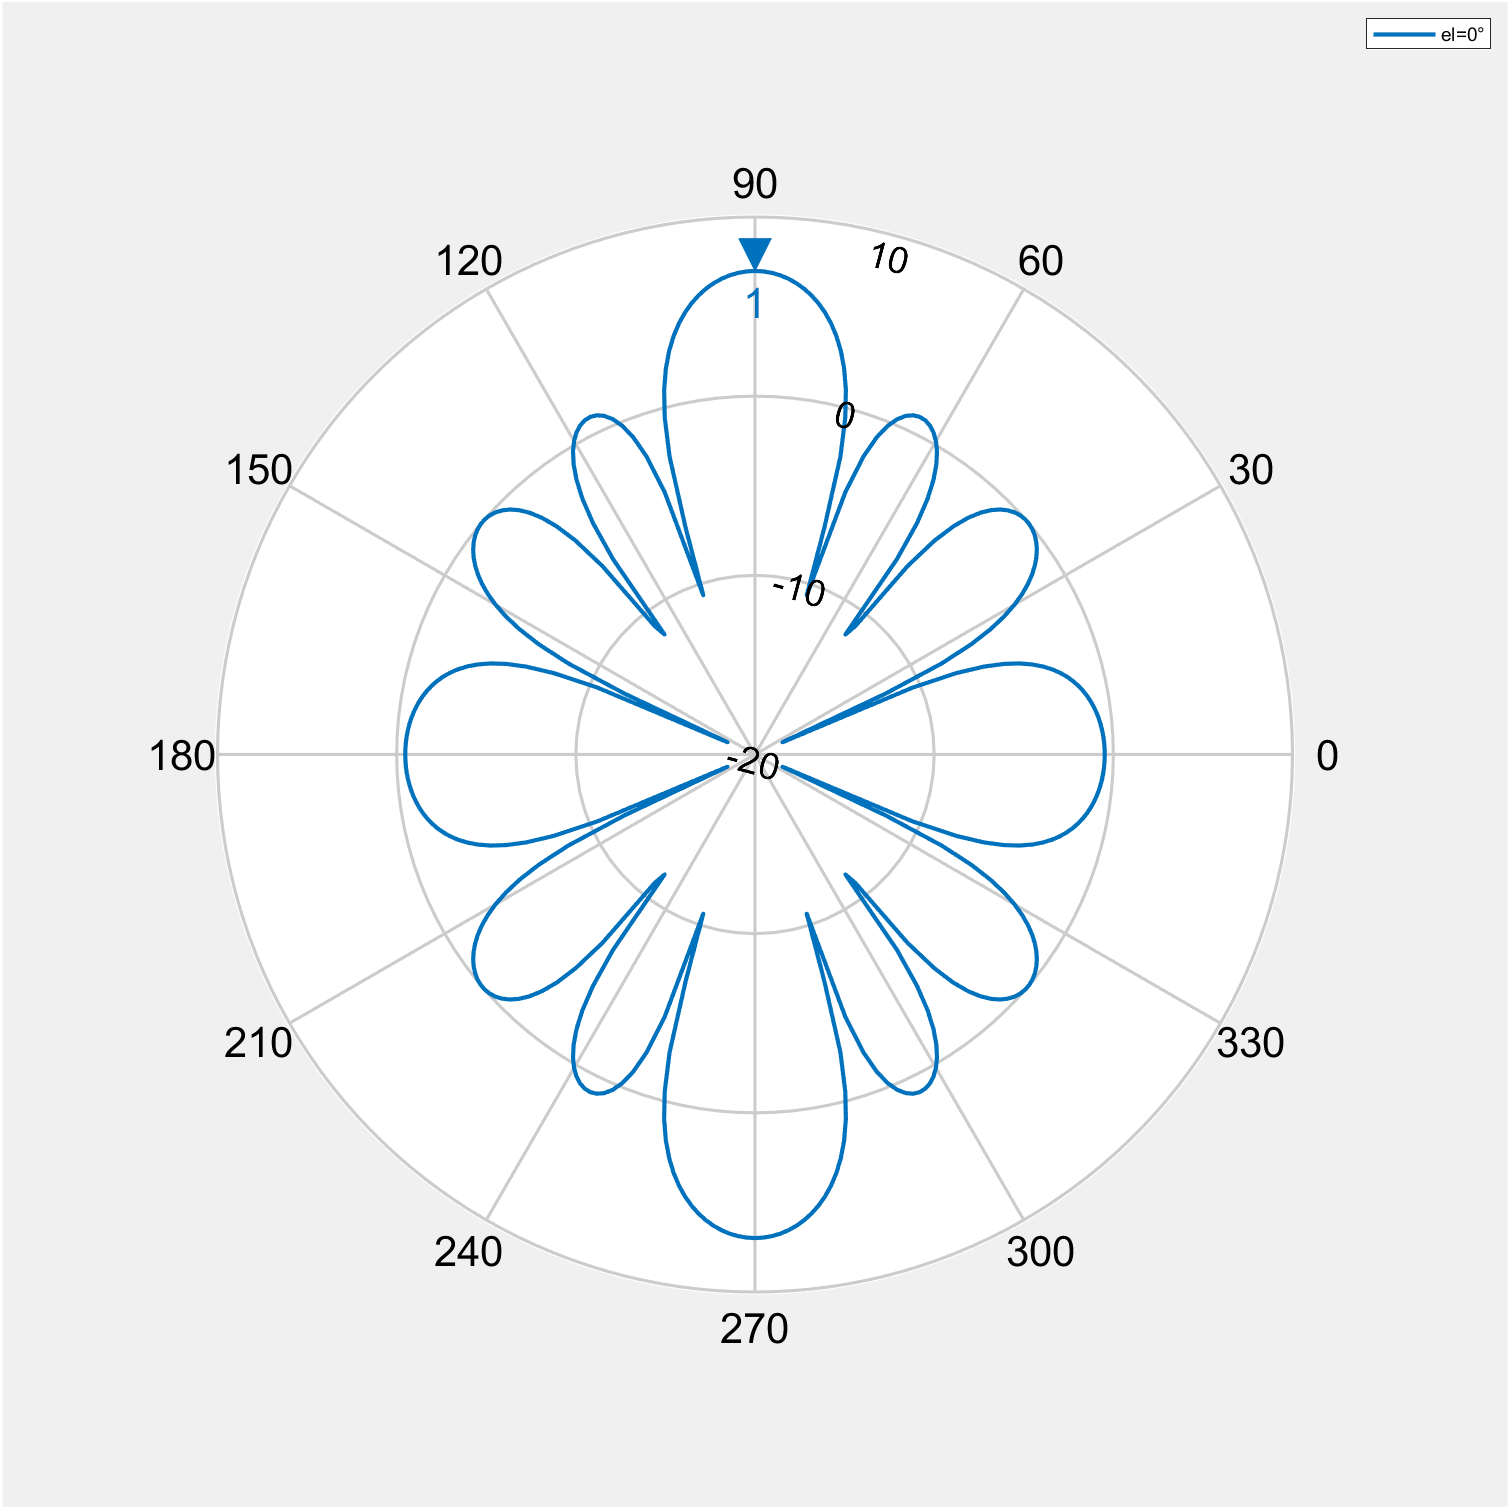
\includegraphics[scale=0.3]{array_factor_polar.png}
	\end{subfigure}
			\hfill
	\begin{subfigure}{0.55\linewidth}
		\def\svgwidth{\linewidth}
		\tiny{\input{pcb_array_factor_with_toolbox_rectangular_az_tex.pdf_tex}}
		\caption{}
			\end{subfigure}
			\hfill
	\begin{subfigure}{0.4\linewidth}
		\def\svgwidth{\linewidth}
		\tiny{\input{pcb_array_factor_with_toolbox_polar_el_tex.pdf_tex}}
	\caption{}
		%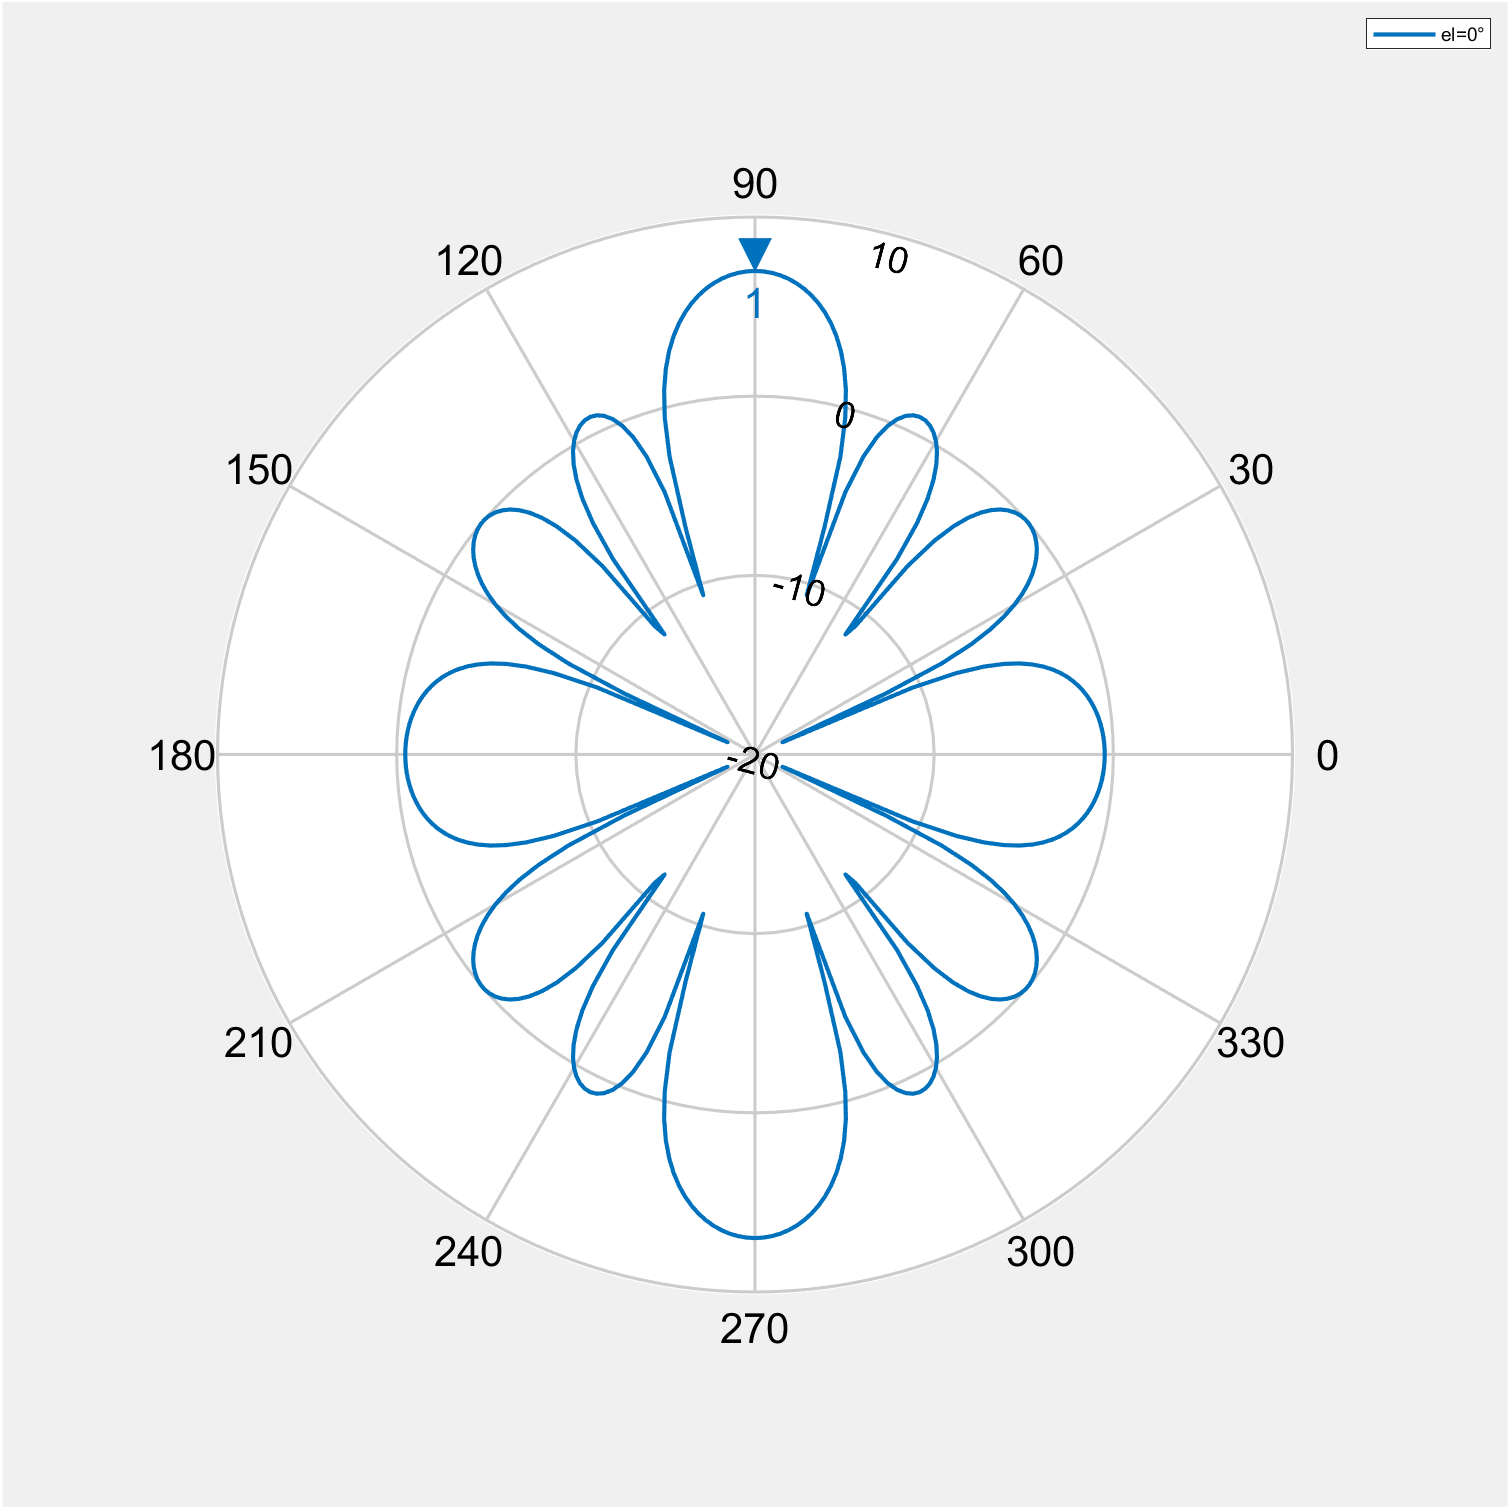
\includegraphics[scale=0.3]{array_factor_polar.png}
	\end{subfigure}
			\hfill
	\begin{subfigure}{0.55\linewidth}
	\def\svgwidth{\linewidth}
\tiny{\input{pcb_array_factor_with_toolbox_rectangular_el_tex.pdf_tex}}
	\caption{}
\end{subfigure}
	\hfill
\caption{{Array factor polar, in azimuth (a) and elevation (c) cut, and rectangular  in azimuth (b) and elevation (d) cut, diagrams}}
\label{fig:array factor}
\end{figure*}



%%% POINT B %%%

\section*{Rectangular folded patch design}

The main components of a rectangular folded patch are: the patch, the substrate (generally accessory, but used in this project), the ground, the rectangular shorting pin between the patch and the ground, and the feed. More details about them will be presented in a short while. Before that, some other remarks are necessary: this antenna will be the element of the array, which will be designed starting actually from a PIFA (\emph{Planar Inverted F Antenna}), given the limitations of the \texttt{\color{Mahogany}Antenna Toolbox}, which will be discussed and overcome later on. A general PIFA realized with a dielectric substrate is shown in \textbf{\cref{fig:patch_structure}}. A particular condition is imposed to the PIFA, by which the width of the rectangular shorting pin ($w_{sc}$) equals the patch width size ($W_{patch}$), so that the PIFA and the folded patch antenna will be two equivalent structures (see \textbf{\cref{eq:shorting condition}}). This remark on the PIFA is necessary because generally its structure is not equivalent to that of the folded patch antenna because of the possible variability of the shorting width ($w_{sc}$), which doesn't always satisfy the above imposed condition. This condition on $w_{sc}$ represents one of the input variables of the PIFA design, such as the matched input resistance ($R_{in}$), the resonant frequency ($f$) and the substrate characteristics (see \textbf{\cref{table:pifa design parameters}}). A preliminary evaluation of the patch parameters have been realized by leaning on a theoretical set of formulas (see \textbf{\cite{Balanis1}}). That's the reason why the characteristics of the patch shown into the \textbf{\cref{table:pifa design parameters}} are called "\emph{pre-optimized features}" (same thing applies to the ground component). Thus, an optimization process of all these and other parameters will be performed in some following steps. Just before that, now the theoretical model will be shortly pointed out: it furnishes a provisional set of results (that will be adjusted afterward) . Firstly length and the width of the patch starting from the $w_{sc}=W_{patch}$ imposed condition, the substrate wavelength and thickness (i.e. $\lambda_{FR4}$ and $h_{FR4}$) are calculated (\textbf{\cref{eq:patch size}}). Then, other parameters, such as the effective permittivity $\varepsilon_{eff}$  and length ($L_{eff}$) in \textbf{\cref{eq:patch effective}}, the radiation resistance ($R_r$) in \textbf{\cref{eq:radiation resistance}}, the half-power beamwidth in the E-cut ($\Theta_E$) and the H-cut ($\Theta_H$) in \textbf{\cref{eq:beamwidth EH cuts}} and eventually the feed location ($\ell_{feed}$) in the patch length direction with respect to the free edge (\textbf{\cref{eq:feed length coordinate}}) have been calculated. 
\subsection*{Refinement with \texttt{\color{BurntOrange}MatLab MoM}}
\subsection*{Substrate thickness selection}Three thickness levels were available for the $FR4$ substrate required in this project (see \textbf{\cref{table:substrate tchickness}}). In this part it will be explained why choosing a thinner substrate (if the $FR4$ is used) is more convienient. This choice will be motivated both in relation to the physical behaviour (radiation efficiency) and to the limits of the \texttt{\color{BurntOrange}Matlab} tools that have been used (in terms of the mesh density level selection in a range that gives more reliable results). 

The \texttt{\color{Mahogany}Antenna Toolbox} gives specific
information about the mesh density level that should be adopted for the design of the patch antenna components. The only issue is that these details are given only for particular ranges of the ratio indicator called \emph{relative thickness} or \emph{electrical thickness} $h_{\lambda}$ (see \textbf{\cite{makarov}}). The electrical thickness depends on the ratio between the substrate thickness ($h_{FR4}$) and the wavelength related to the substrate medium ($\lambda_{FR4}$). When a mesh is configured in the \texttt{\color{Mahogany}Antenna Toolbox} environment, a specific parameter needs to be adjusted: the maximum edge length of the generic triangle covering the geometry of the antenna ($e_{\max}$). In the case of a relative length $h_\lambda$ comparable to $1/10$, it's recommended to select an $e_{\max}\,\cong\,\lambda/10$. A substrate thickness respecting this relationship is called a \emph{thick substrate}. None of the available substrates verifies this condition. Among them, only the thinnest substrate and the second to last one (thus $h_{FR4}=0.8\,mm$ and $h_{FR4}=1.0\,mm$) are part of a range which the \texttt{\color{Mahogany}Antenna Toolbox} provides instructions of. It's the \emph{thin substrate range}: the automatic mesh mode should be adopted for a thin substrate, namely having a relative thickness less or equal than one fifth ($h_\lambda\,\leq{1/50}$). An evaluation of the $h_\lambda$ of two substrates respecting this condition is shown in \textbf{\cref{eq:substrate relative thickness}}. This leads to a full explanation of actual substrate thickness chosen for this project. The thinner substrate choice rationale starts with the consideration of its quality factor ($Q$) depending on the loss tangent ($tan\delta$) is generally low in the FR4 substrate case (being the two quantities inversely proportional, i.e. $Q\,\propto\,1/tan\delta$, and being $(\tan\delta)$ very high compared to that of other more efficient substrates). This means the FR4 is a big power dispersor. Since increasing $h_{FR4}$ will provoke just more losses in terms of a radiation efficiency drop and since the only thickness values of $0.8\,mm$ and $1.0\,mm$ would give reliable/accurate results in the \texttt{\color{Mahogany}Antenna Toolbox} simulations, the $0.8\,mm$ tchickness level will be adopted. 
\subsection*{Mesh density refinement}
Although a mesh density choice has already been made by selecting the best maximum edge length $e_{\max}$, the accuracy achievable by using the mesh automatic mode in the case of substrates belonging to the  \emph{thin substrate range} will be proved hereafter. An initial study of the mesh density level influence on the reflection coefficient ($\Gamma$ in $dB$) evaluated at the resonant frequency ($f=2.1\,GHz$) has been realized, thus a  $\Gamma_{2.1\,GHz}=F(e_{\max})$ function has been plotted with an initial step of $\Delta e_{\max} = 2.5^.1^{-4}\,m$ between every two mesh densities related to their specific $e_{\max}$. This first simulation considered a broader range of $e_{\max}$ variation: $[2.5^.10^{-4}\,m\,,\,6.0^.10^{-4}\,m]$. 

\indent 

Since the resulting plot  (\textbf{\cref{fig:first mesh test}}) has shown big uncertainty of the reflection coefficient value at the resonant frequency ($\Gamma_{2.1\,GHz}$) at almost every mesh $e_{\max}$ level (primarily due to the big step selected between one density level and another), some more detailed tests have been run, by considering a slightly narrower range ($[2.5^.10^{-4}\,m\,,\,5.0^{-4}\,m]$) and a tchicker evaluation of the maximum edge values (so that the mesh variation step has been remarkably reduced to $1.0^{-4}\,m$). Specifically, the step between two mesh density levels in terms of the maximum edge length of each one has been reduced from a $\Delta e_m=2.5^.10^{-4}$ to $\Delta e_m=1.0^.10^{-4}$. In all those simulations, an important fact needs to be noted. Even very small variations on the maximum edge length value involved considerable inconsistencies in almost every part of the mesh range in terms of considerable variations of the frequency at wich $\Gamma$ reaches its minimum ($\min(\Gamma)$, therefore the resonant frequency of the antenna changes very easily).  
Thus, considering the frequency $f^*$ at which $\min(\Gamma)$ is actually obtained, instead of evaluationg it at the theoretical resonating frequency value at every mesh level, not only the standard test comparing $e_{\max}$ and $\Gamma$ has been run, but also some mesh refinement plots representing the relationship between $f^*$ and $e_{\max}$ (\textbf{\cref{eq:f vs mesh}}), $\Delta f^*$ and $e_{\max}$ (\textbf{\cref{eq:Df vs mesh}}) and also $\min(\Gamma)$ and $e_{\max}$ (\textbf{\cref{eq:minG vs mesh}}) have been taken into account (where $\Delta f^*$ is the difference between $f^*$ and the resonant frequency $f=2.1\,GHz$). More parameter relationships have been collected and this led to the setting of the mesh density choice in terms of $e_{\max}$ that has been selected inside the most stable region (i.e. showing the smallest deviation of the reflection coefficient minimum from the resonant frequency). In the end it's been specifically taken the 'automatic' $e_{\max}$ ($=3.5^{-4}\,m$) suggested by the \texttt{\color{Mahogany}Antenna Toolbox}, since this value  belongs to the stable region and seems to give the most accurate results. The $e_{\max}$ values belonging to the stable region ($[3.1\,^.\,10^{-4}\,m,3.7^.10^{-4}\,m]$) exibit slight deviations from the resonant frequency ($\Delta f^*\,\in\,[0.01\,GHz,0.03\,GHz]$) and the minimum of the reflection coefficient varies in the range $[-24\,dB\,,\,-33\,dB]$. 
\subsection*{Patch parameters refinement}
After the selection of the maximum edge length of the mesh (consequently, of its density level), a more refined computation of the reflection coefficient will be made, depending on the patch size (i.e. on its length and width), but also on the feed location. Firstly, only a parametrical variation of the feed position across the patch length direction has been considered, depending on variations of $L_{patch}$ and $W_{patch}$. This means that the first refinement of the feed position has been evaluated starting from its theoretical equation (depending indirectly by $W_{patch}$). The change of the feed location has been taken into account in the computation of every step of the simulation, thus in every evaluation of the reflection coefficient, keeping $e_{\max}$ as a constant (the previously selected length). The patch size variations provoked wide modifications of the reflection coefficient, which values depending on that have been represented by an initial contour plot (with variations of the patch size in a broader range and with a larger step between one value and another, see \textbf{\cref{fig:first contour}}). After that, another simulation (\textbf{\cref{fig:second contour}}) in a narrower range of the patch size variation has been run in order to choose from there a set of $\Gamma$ values (i.e. a set of coupled values $(L_{patch},W_{patch})$) that should put the patch antenna in the best resonant condition (which means that a $\Gamma$ as close as possible to zero in the linear scale and as negative as possible in the $dB$, logarithmic scale is sought). The logarithmic ($dB$ scale) was used for the contour plots because this way the resulting $\Gamma$ values are easier to distinguish from one another even grafically and mathematically. 
%%%%%%%%%%%%%%%%%%%%%%%%%%%%%%%%%%%%%%%%%%%%%%%%%%%%%%%%%
%%%%%%%%%%%%%%%%%%%%%%%%%%%%%%%%%%%%%%%%%%%%%%%%%%%%%%%%%
%% se c'è tempo e spazio ancora nella relazione %%%%%%%%%
%% discutere anche sul VSWR %%%%%%%%%%%%%%%%%%%%%%%%%%%%%
%% che dev'essere il più vicino ad 1 %%%%%%%%%%%%%%%%%%%%
%%%%%%%%%%%%%%%%%%%%%%%%%%%%%%%%%%%%%%%%%%%%%%%%%%%%%%%%%
%%%%%%%%%%%%%%%%%%%%%%%%%%%%%%%%%%%%%%%%%%%%%%%%%%%%%%%%%
A set of 20 values of $\Gamma$ and respective coupled values ($L_{patch},W_{patch}$). has been selected from the second simulation range so that a more specific simulation could be run. In this third case (\textbf{\cref{fig:Gamma couple LpWp}}), the reflection coefficient has been plotted in a range around the resonant frequency ($[2.0\,GHz, 2.2\,GHz]$) in order to find which is the best combination for the patch size that makes actually resonate the antenna at the project frequency. Another determining and discriminating factor was the input impedance ($Z_{in}=R_{in}+\jmath Y_{in}$, where the real part of $Z_{in}$ is the imput resistance, while the imaginary one is the input reactance), because a impedance matching (at $50\,\Omega$) needed to be achieved for the project. In the ideal case, of course, a reflection coefficient $\Gamma^{(id)}=0.00\,\to\,-\infty\,dB$ would be required in order to reach the perfect impedance matching (perfect matching with input resistance at $50.00\,\Omega$ and null reactance). As an actual result, before seeking a better matching, the $\Gamma$ value related to all the couple candidates ($(L_{patch},W_{patch})$) spaced ranged from $-24\,dB$ to $-30\,dB$. The two best candidates of the $\Gamma$ value related to the coupled size ($L_{patch},W_{patch}$) are plotted in \textbf{\cref{fig:Gamma couple LpWp}}. Two refined plots (with narrower frequency steps in the same range) of $\Gamma$ and $Z$ for one of the candidates are represented in \textbf{\cref{fig:Gamma and Z previa wfeed}}. An additional design strategy contributed to the final patch size choice: the feed location varying across the patch width direction ($w_{feed}$). Thus, a parametrical impedance matching study depending on that has been run on the best couple candidates and a few others from the set of 20. The resulting values are listed in \textbf{\cref{table:Gamma and Z}} and the plots are shown in \textbf{\cref{fig:Gamma and Z}}

\begin{figure*}[bt!]
	\begin{subfigure}{0.3\linewidth}
		\def\svgwidth{\linewidth}
		\tiny{\input{patch_structure_tex.pdf_tex}}
	\end{subfigure}
	\hfill
	\begin{subfigure}{0.3\linewidth}
		\def\svgwidth{\linewidth}
		\tiny{\input{patch_structure_2_tex.pdf_tex}}
	\end{subfigure}
	\hfill
	\begin{subfigure}{0.3\linewidth}
		\def\svgwidth{\linewidth}
		\tiny{\input{patch_structure_3_tex.pdf_tex}}
	\end{subfigure}
	%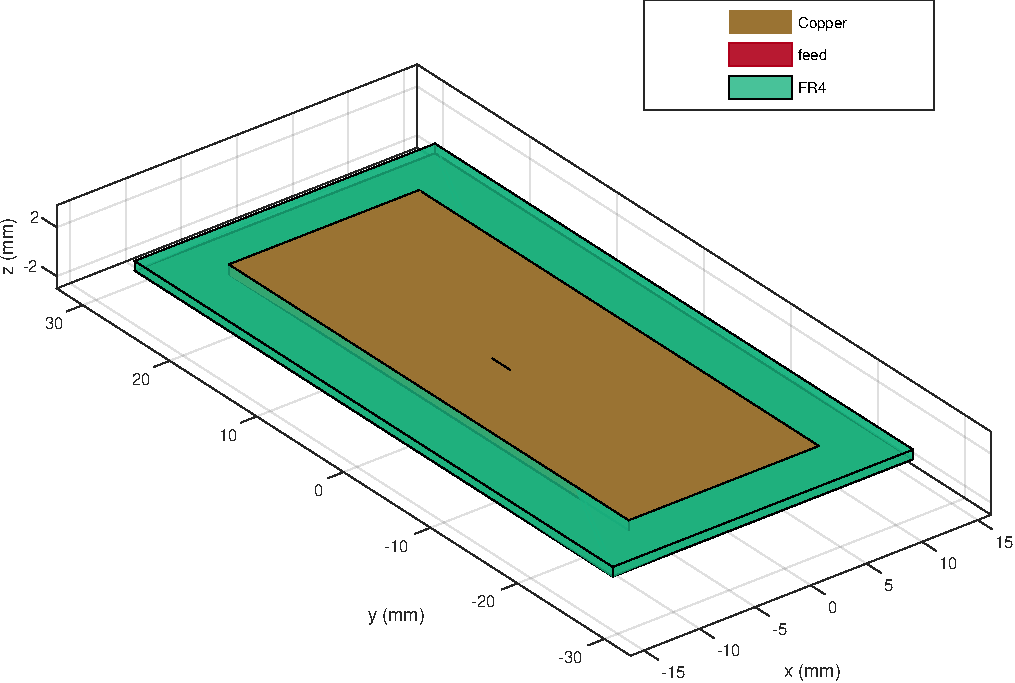
\includegraphics[scale=0.35]{patch_structure.pdf}
	%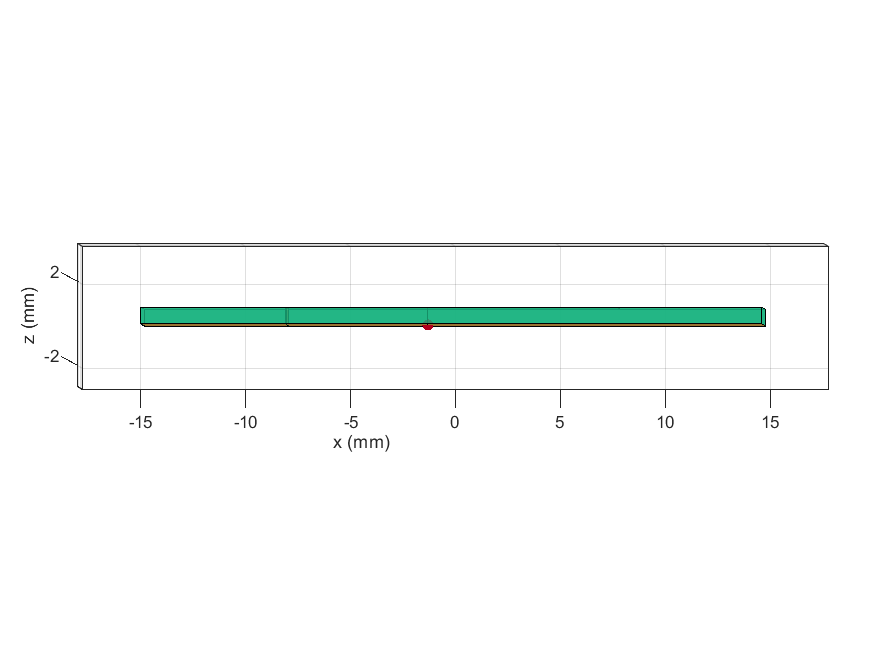
\includegraphics[scale=0.35]{patch_structure_2.pdf}
	%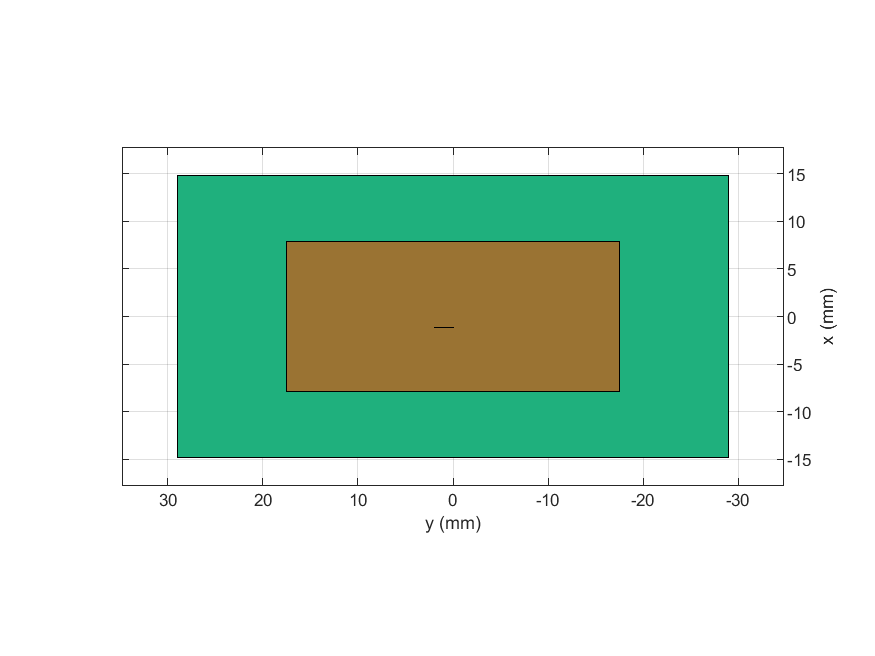
\includegraphics[scale=0.35]{patch_structure_3.pdf}
	
	\caption{PIFA realized with a dielectric substrate}
	\label{fig:patch_structure}
\end{figure*}

\begin{equation}
	W_{patch}\,=\,w_{sc}
	\label{eq:shorting condition}
\end{equation}

	\begin{table}[bt!]
		\begin{center}
		% \FloatBarrier
			{\fontfamily{lmss}\selectfont
\begin{tabular}{||m{4.2cm}|m{4.2cm}||}
\hline 
	\rowcolor{lightgray}\multicolumn{2}{|c|}{\textbf{Folded patch design parameters}} 
	\\
	\hline
	\cellcolor{mintbg}\textbf{Parameter/Component} & \cellcolor{mintbg}\textbf{Value/Type/Material}\\
	\hline
	Frequency & $2.1\,GHz$ \\
	\hline
	Matched input resistance & $R_{in}\,=\,50\,\Omega$\\
	\hline
	\cellcolor{pink} Substrate & \cellcolor{pink} FR4 \\
	\hline
    Relative permittivity & $\varepsilon_{FR4}\,=\,4.8$ \\

	Relative permeability & $\mu_{FR4}\,\cong\,1$\\

	Loss tangent & $\{\tan(\delta)\}_{FR4}\,=\,0.0260$\\

	Thickness & $h_{FR4}\,=\,0.8\,mm$\\
	\hline
\cellcolor{pink} Patch

(pre-optimized features) & \cellcolor{pink} Copper \\
\hline
%\begin{subtable}{0.25\textwidth}
%	\begin{tabular}{|c|c|}
%		\hline
%		try & c\\
%		\hline
%	\end{tabular}
%	
%	\end{subtable} & \\
%\hline
Conductivity & $\kappa_{copper}\,=\,5.96^.10^7\,S/m$ \\

Thickness & $h_{patch}\,=\,3.556\,^.\,10^{-5}\,m$\\

Length & $L_{patch}\,\cong\,\frac{\lambda_{FR4}}{4}\,=\,0.0171\,m$\\

Width & $W_{patch}\,\cong\,0.419\,m$\\

	\hline
\cellcolor{pink}Ground 

(pre-optimized features)
& \cellcolor{pink} Copper

(same conductivity listed above) \\
\hline
Thickness & $h_{GND}\,=\,h_{patch}$
\\
Length & $L_{GND}\,=\,0.04\,m$\\
Width & $W_{GND}\,=\,0.06\,m$\\
\hline
\cellcolor{pink}Feed & \cellcolor{pink} Coaxial cable \\
\hline
\end{tabular}}
\caption{Project input parameters (frequency, matching and substrate features) and theoretical (pre-optimized) features of the patch and ground PIFA components}
\label{table:pifa design parameters}
\end{center}

\end{table}

\begin{equation}
	\begin{aligned}L_{patch}\,+\,W_{patch}\,-\,w_{sc}\,&{\color{Mahogany}=}\,\frac{\lambda_{FR4}}{4}\,+\,h_{FR4}\\
		W_{patch}\,&{\color{Mahogany}=}\,\frac{\lambda}{2}\,\sqrt{\frac{2}{\varepsilon_{FR4}\,+\,1}}\\
	\end{aligned}
\label{eq:patch size}
\end{equation}
\begin{equation}
	\begin{aligned}
		\varepsilon_{eff}\,{\color{Mahogany}=}\,\frac{\varepsilon_{FR4}+1}{2}\,+\,\frac{\varepsilon_{FR4}-1}{2}\,\left(1+12\frac{h_{FR4}}{W_{patch}}\right)^{-\frac{1}{2}}\\
		L_{eff}\,{\color{Mahogany}=}\,\frac{\lambda_{FR4}}{4}\\
		\Delta L{\color{Mahogany}=}0.412\,h\,\left[\frac{(\varepsilon_{eff}+0.3)\,\left(\frac{W_{patch}}{h_{FR4}}+0.268\right)}{(\varepsilon_{eff}-0.258)\,\left(\frac{W_{patch}}{h_{FR4}}+0.8\right)}\right]\\
		L\,=\,L_{eff}-2\Delta L
	\end{aligned}
\label{eq:patch effective}
\end{equation}
\begin{equation}
R_r\,{=}\,\frac{120\,\lambda}{W_{patch}}\,\left[1-\frac{1}{24}\,\left(2\pi\,\frac{h_{FR4}}{\lambda}\right)^{2}\right]^{-1}\\
\label{eq:radiation resistance}
\end{equation}
\begin{equation}
	\begin{aligned}
		\Theta_E\,&{\color{Mahogany}=}\,2\,\arccos\,\sqrt{\frac{7.03\,\lambda^2}{4\,(3\,L_e^2+h_{FR4}^2)\,\pi^2}}\\
		\Theta_H\,&{\color{Mahogany}=}\,2\,\arccos\sqrt{\frac{1}{2\,+\,2\pi\,\frac{W_{patch}}{\lambda}}}\\
	\end{aligned}
\label{eq:beamwidth EH cuts}
\end{equation}
\begin{equation}
	\ell_{feed}\,{\color{Mahogany}=}\,\frac{L_{patch}}{\pi}\,\arccos\,\sqrt{\frac{R_{in}}{R_r}}
	\label{eq:feed length coordinate}
\end{equation}

%%%%%%%%%%%%%%%%%%%%%%%%%%%%%%%
%%%%%%%%%%%%%%%%%%%%%%%%%%%%%%%
%%%%%%%%%%%%%%%%%%%%%%%%%%%%%%%
%%%%%%%%%%%%%%%%%%%%%%%%%%%%%%%
%%%%%%%%%%%%%%%%%%%%%%%%%%%%%%%
%%%%%%%%%%%%%%%%%%%%%%%%%%%%%%%
%%%%%%%%%%%%%%%%%%%%%%%%%%%%%%%
%%%%%%%%%%%%%%%%%%%%%%%%%%%%%%%
%%%%%%%%%%%%%%%%%%%%%%%%%%%%%%%
%%%%%%%%%%%%%%%%%%%%%%%%%%%%%%%
%%%%%%%%%%%%%%%%%%%%%%%%%%%%%%%
%%%%%%%%%%%%%%%%%%%%%%%%%%%%%%%
	\begin{table*}[bt!]
	\begin{center}
		%%% \FloatBarrier
		{\fontfamily{lmss}\selectfont
			\begin{tabular}{||m{3cm}|m{3cm}|m{3cm}||}
				\hline 
				\rowcolor{lightgray}\multicolumn{3}{|c|}{\textbf{FR4 substrate project thickness levels available}} 
				\\
				\hline
				\cellcolor{pink}$h_{FR4}^{(1)}=0.8\,mm$ & 
					\cellcolor{pink}$h_{FR4}^{(2)}=1.0\,mm$ & 
						\cellcolor{pink}$h_{FR4}^{(3)}=1.6\,mm$  \\
				\hline
				
			\end{tabular}}
		\caption{Three levels of $FR4$ substrate thickness are shown above. In the antenna industry, the $FR4$ substrate thickness generally ranges from $0.8\,mm$ and $3.6\,mm$}
	\label{table:substrate tchickness}\end{center}\end{table*}
\begin{equation}\begin{aligned}
	h_{FR4} &= 0.8\,mm\,\leadsto\,h_{\lambda}\,=\,\frac{1}{81}\\	h_{FR4} &= 1.0\,mm\,\leadsto\,h_{\lambda}\,=\,\frac{1}{62}\\
\end{aligned}
	\label{eq:substrate relative thickness}
\end{equation}
%\begin{center}
%	\fbox{\begin{minipage}{0.7\linewidth}
%\textbf{\color{Mahogany}\emph{Thinner substrate choice} rationale}. The quality factor depending on $tan\delta$ is generally low in the FR4 substrate case. This means the FR4 is a big power dispersor. Since increasing $h_{FR4}$ will provoke just more losses in terms of a radiation efficiency drop and since the only thickness values of $0.8\,mm$ and $1.0\,mm$ would give reliable/accurate results in the \texttt{\color{Mahogany}Antenna Toolbox} simulations, the $0.8\,mm$ will be adopted.
%	\end{minipage}}
%\end{center}
%%%%%%%%%%%%%%%%%%%%%%%%
%%%%%%%%%%%%%%%%%%%%%%%%
%%%%%%%%%%%%%%%%%%%%%%%%%
%%%%%%%%%%%%%%%%%%%%%%%%%
%%%%%%%%%%%%%%%%%%%%%%%

\begin{figure}[bt!]
	%	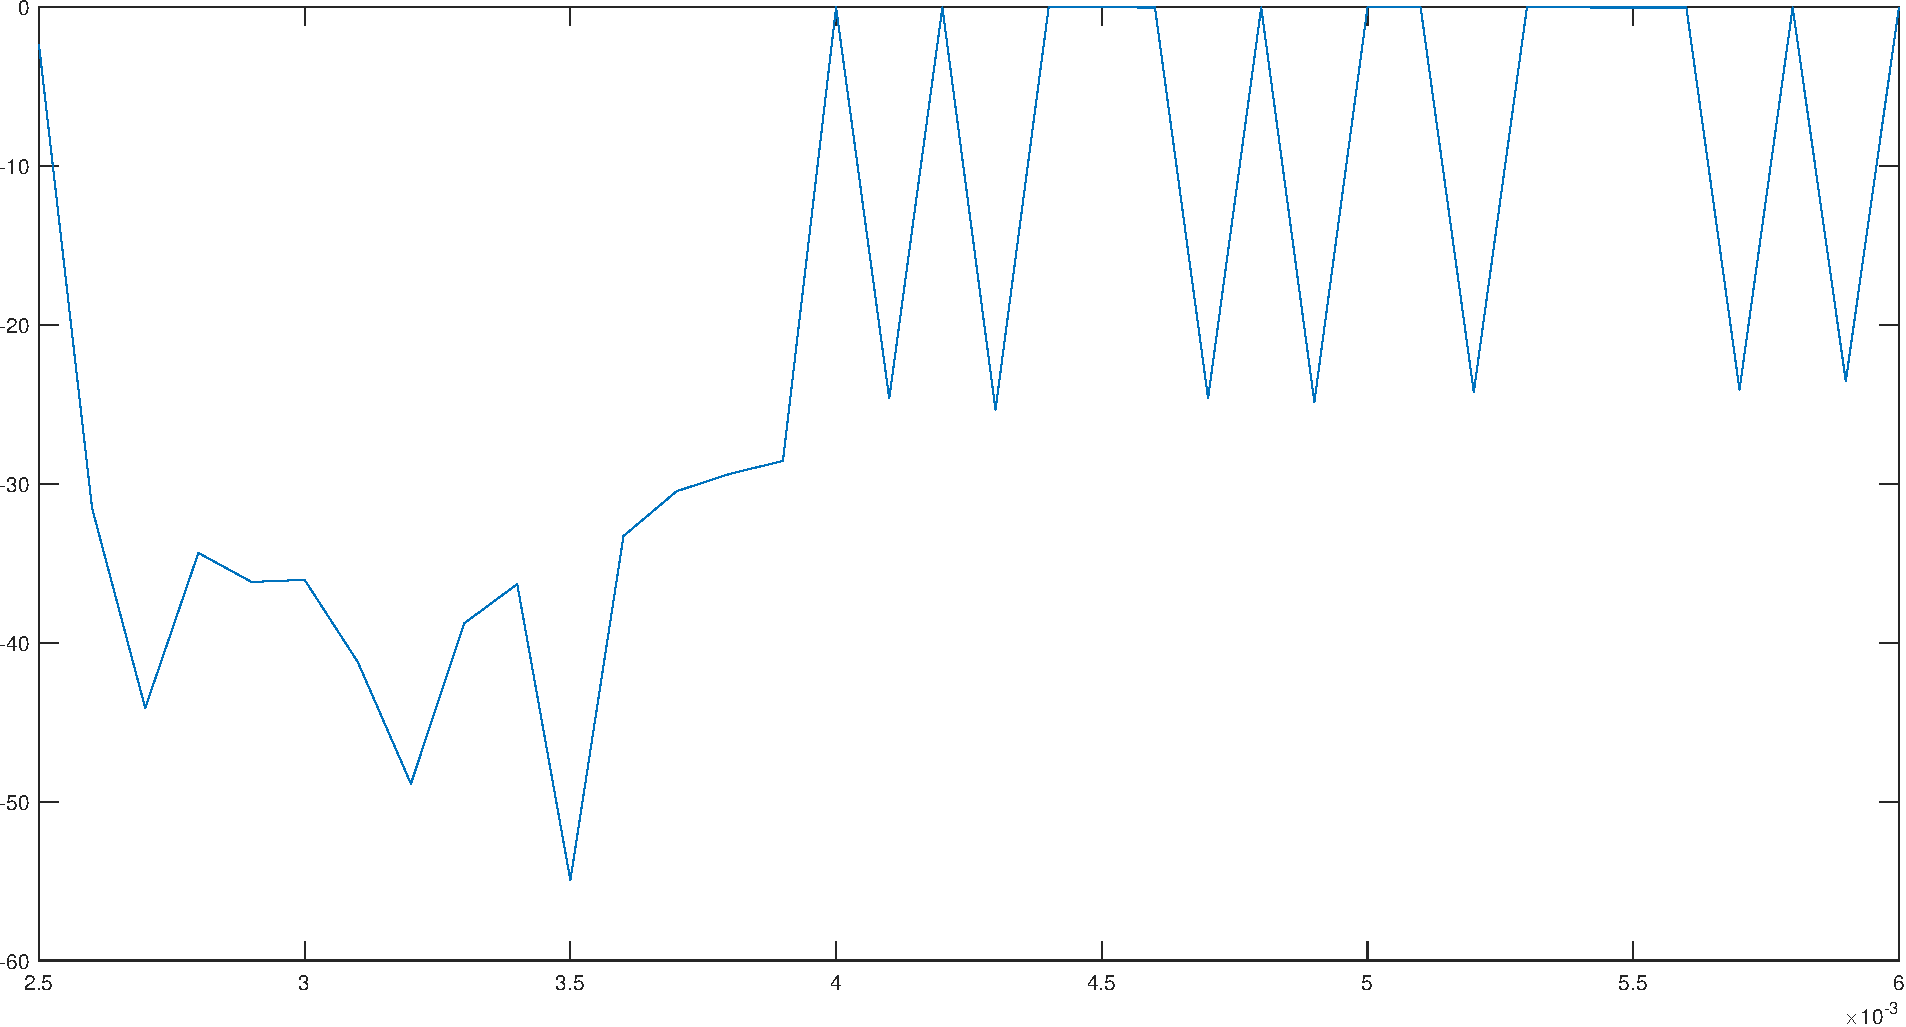
\includegraphics[scale=0.3]{mesh_first_test.pdf}
	\def\svgwidth{\linewidth}
	\tiny{\input{mesh_first_test_tex.pdf_tex}}
	\hfill
	\caption{{Minimum of the reflection coefficient $\Gamma\, [dB]$ in the frequency range $2.0\div 2.2\,GHz$ depending on the varying mesh density level}}
	\label{fig:first mesh test}
\end{figure}

\begin{figure*}[bt!]
	\begin{center}
		\begin{subfigure}[t]{0.32\linewidth}
			\def\svgwidth{\linewidth}
			\tiny{\input{minGamma_vs_mesh_level_tex.pdf_tex}}
			%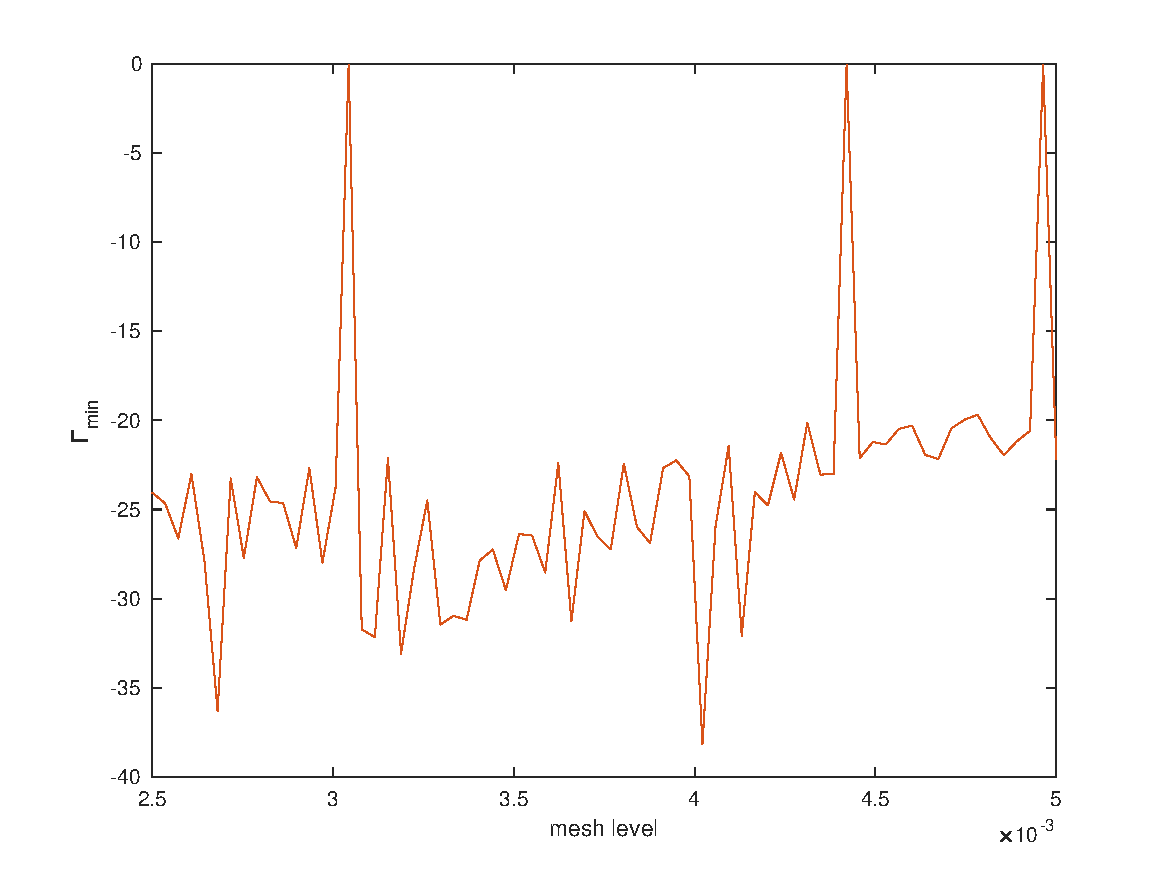
\includegraphics[scale=0.3]{minGamma_vs_mesh_level.pdf}
			\caption{}
			\label{eq:minG vs mesh}
		\end{subfigure}
		\hfill
		\begin{subfigure}[t]{0.32\linewidth}
			%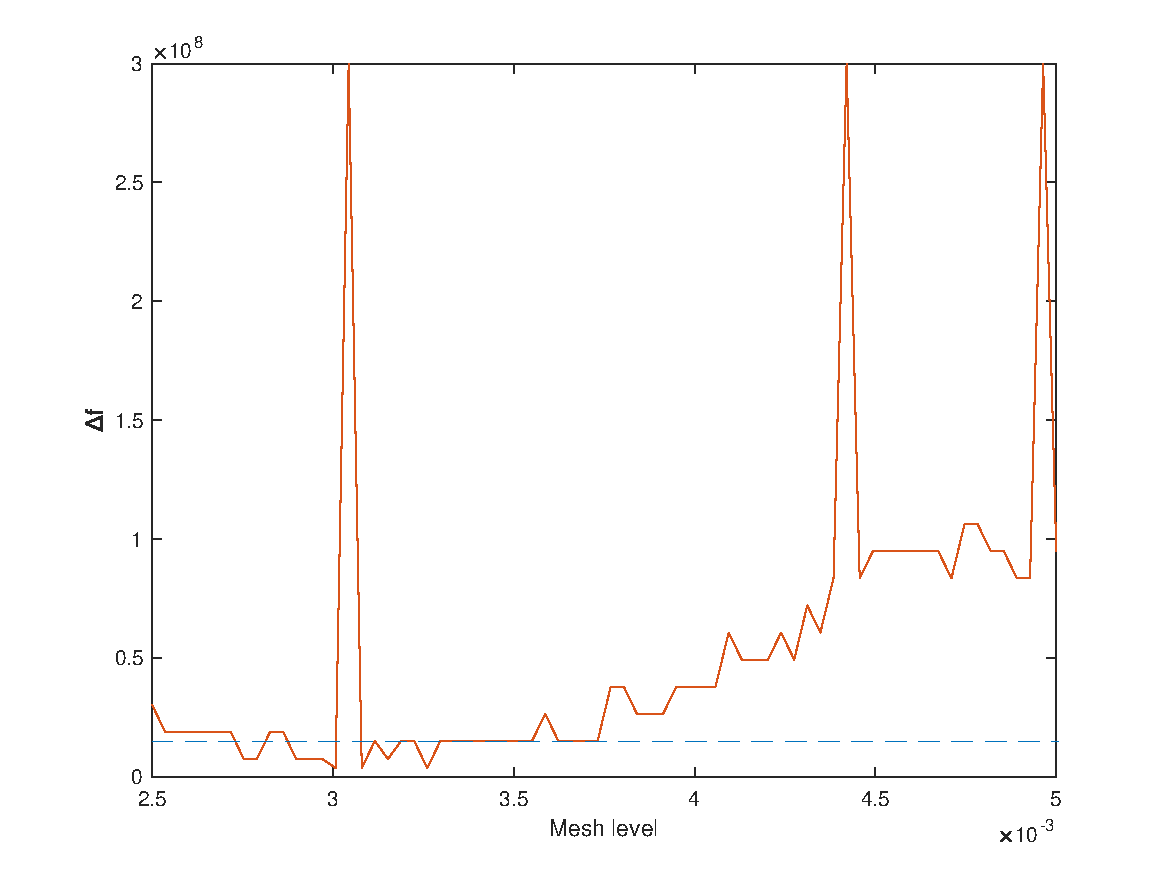
\includegraphics[scale=0.3]{DeltaF_vs_mesh_level.pdf}
			\def\svgwidth{\linewidth}
			\tiny{\input{DeltaF_vs_mesh_level_tex.pdf_tex}}
			
			\caption{}
			\label{eq:Df vs mesh}
		\end{subfigure}
		\hfill
		\begin{subfigure}[t]{0.32\linewidth}
			%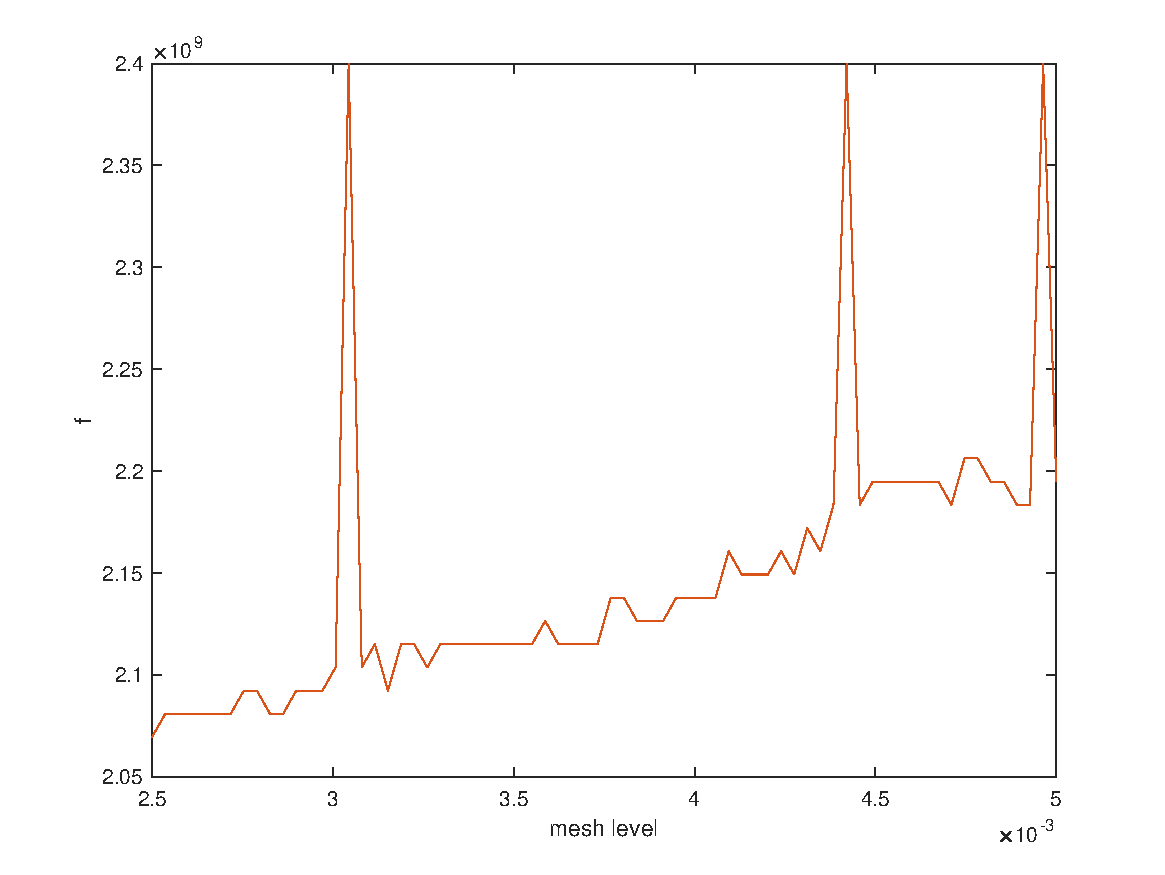
\includegraphics[scale=0.3]{F_vs_mesh_level.pdf}
			\def\svgwidth{\linewidth}
			\tiny{\input{F_vs_mesh_level_tex.pdf_tex}}
			
			\caption{}
			\label{eq:f vs mesh}
		\end{subfigure}
		\hfill
		\caption{Comparison of the meshing parameter $e_{\max}$ with minimum of reflection coefficient (a), variation of the resonant frequency with respect to the design one (the dotted line represents the value with respect to automatic meshing) (b), resonant frequency identified by the minimum of $\Gamma$ (c)} 
	\end{center}
\end{figure*}
%%%%%%%%%%%%%%%%%%%%%%%%%%%%%
%%%%%%%%%%%%%%%%%%%%%%%%%%%%%
%%%%%%%%%%%%%%%%%%%%%%%%%%%%%
%%%%%%%%%%%%%%%%%%%%%%%%%%%%%
%%%%%%%%%%%%%%%%%%%%%%%%%%%%%
%%%%%%%%%%%%%%%%%%%%%%%%%%%%%

	\begin{figure*}[bt!]
	\begin{subfigure}[t]{0.49\linewidth}
		\def\svgwidth{\linewidth}
		\tiny{\input{gamma_pre_wfeed_tex.pdf_tex}}
		%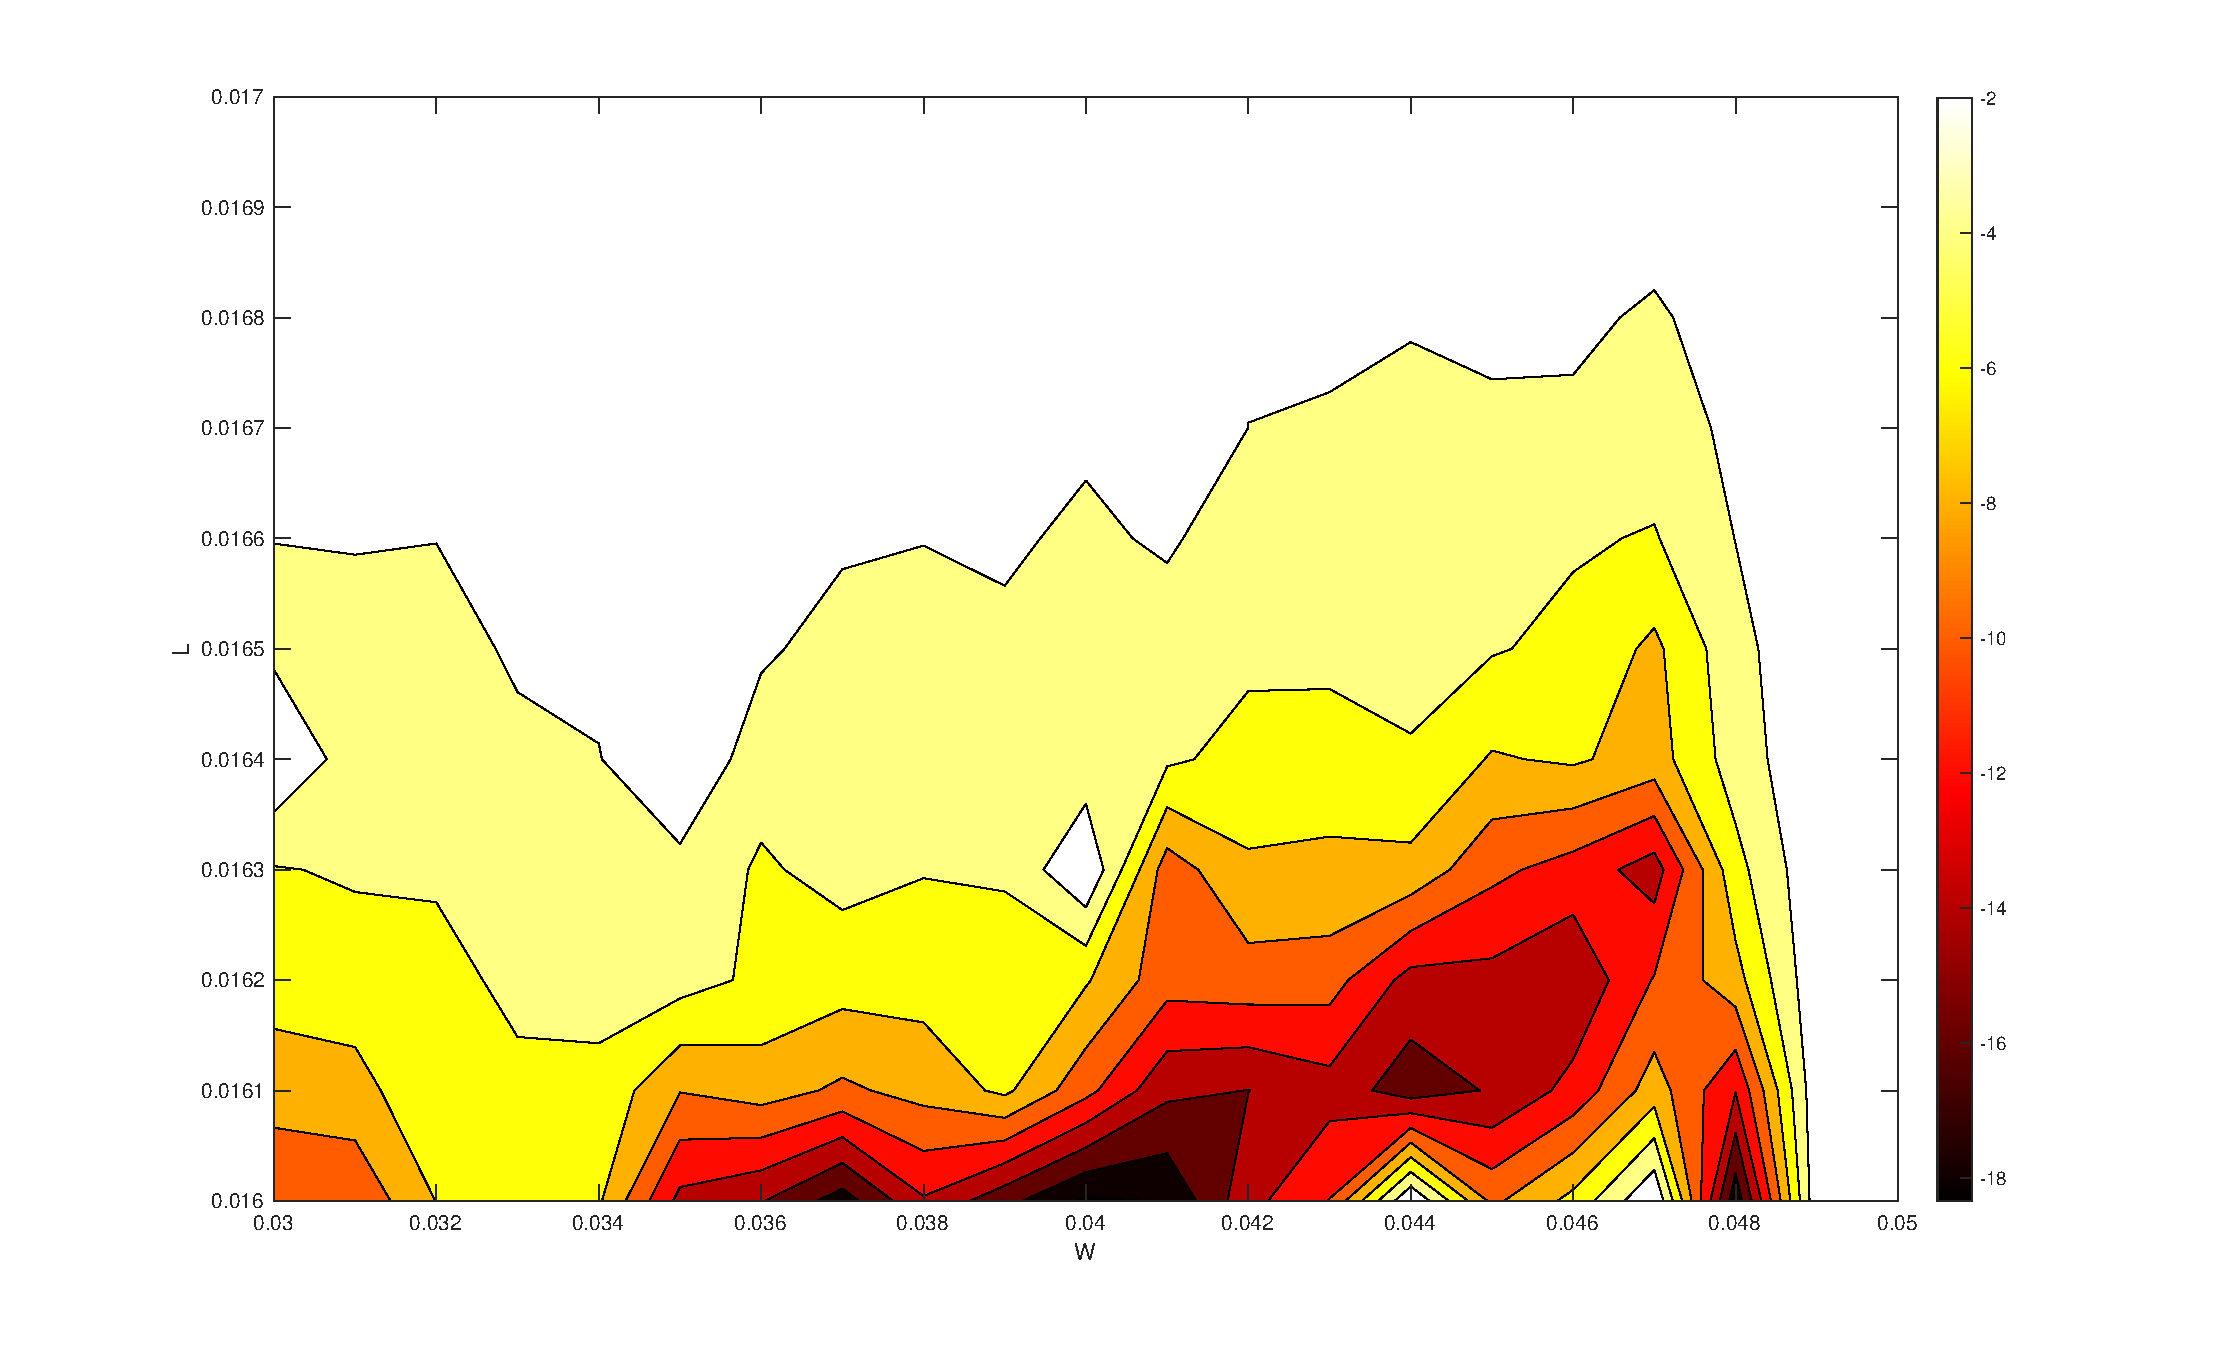
\includegraphics[scale=0.25]{First_Contour_LOG.pdf}
		\caption{}
	\end{subfigure}
	\hfill
	\begin{subfigure}[t]{0.47\linewidth}
		\def\svgwidth{\linewidth}
		\tiny{\input{impedence_pre_wfeed_tex.pdf_tex}}
		%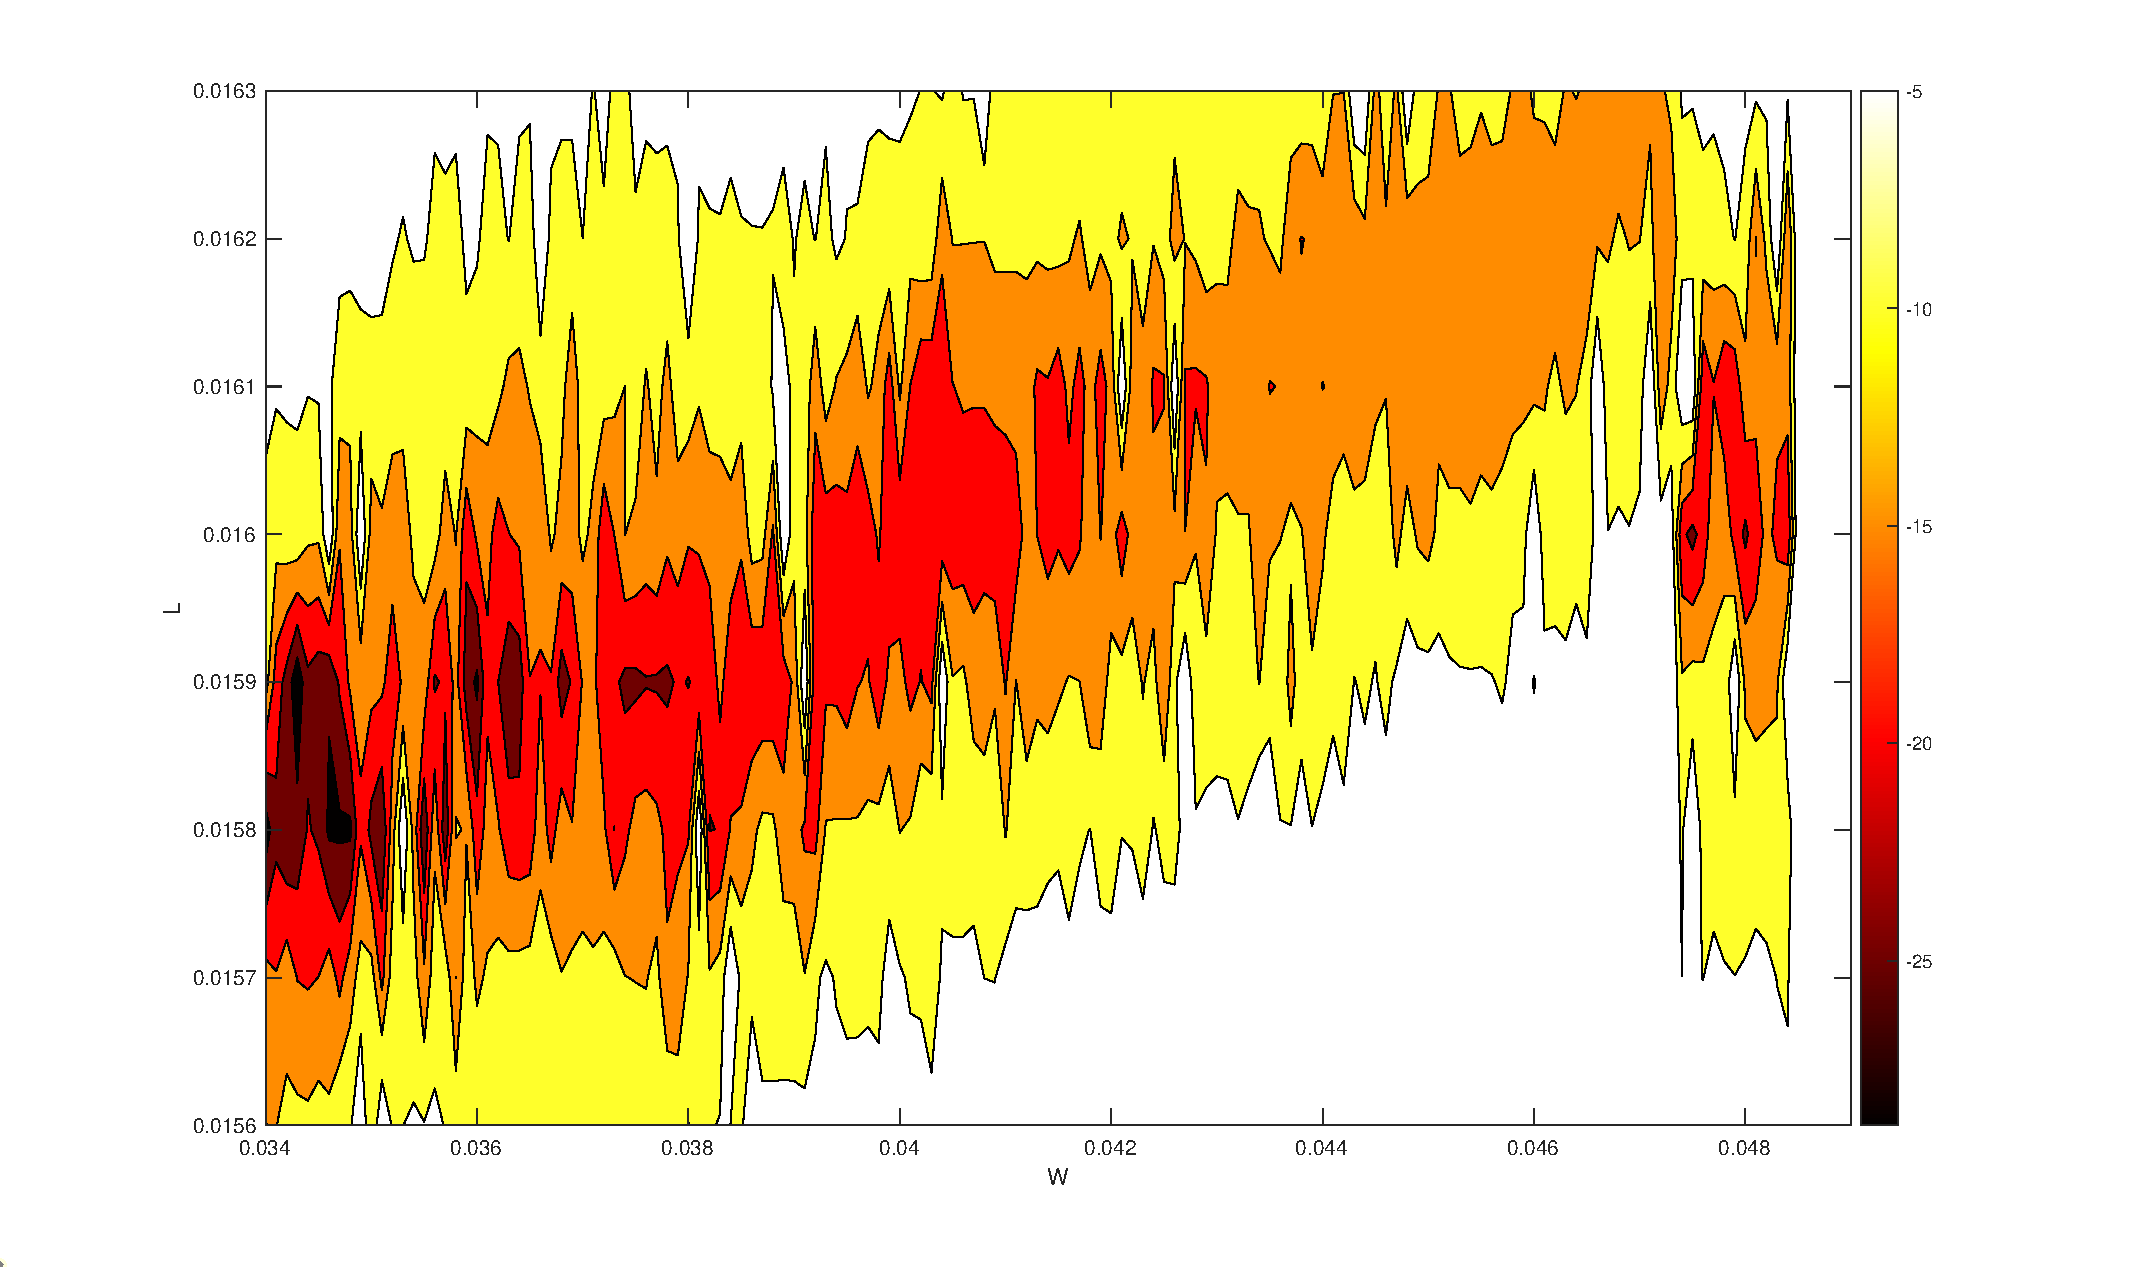
\includegraphics[scale=0.25]{Second_Contour_LOG.pdf}
		\caption{}
	\end{subfigure}
	\caption{Reflection coefficient (a) and impedance (b) plots depending on $f\,\in\,[2.0,2.1\,GHz]$}
	\label{fig:Gamma and Z previa wfeed}
\end{figure*}


\begin{table}
	\begin{center}
	{\fontfamily{lmss}\selectfont	\begin{tabular}{||m{2cm}|m{2cm}||}
\hline
\textbf{Parameter} & \textbf{Value}\\
\hline
	$\Gamma_{final}$ & $-54.94\,dB$\\
	\hline
	 $R_{in}$ & $49.86\,\Omega$ \\
	 \hline
	 $Y_{in}$ & $ 0.11\,S$ \\
\hline
		\end{tabular}}
	\caption{Final $\Gamma$ and impedance matching values after $w_{feed}$ change}
	\label{table:Gamma and Z}
	\end{center}
\end{table}
\begin{figure*}[bt!]
	\begin{subfigure}{0.48\linewidth}
		\def\svgwidth{\linewidth}
		\tiny{\input{First_Contour_LOG_tex.pdf_tex}}
		%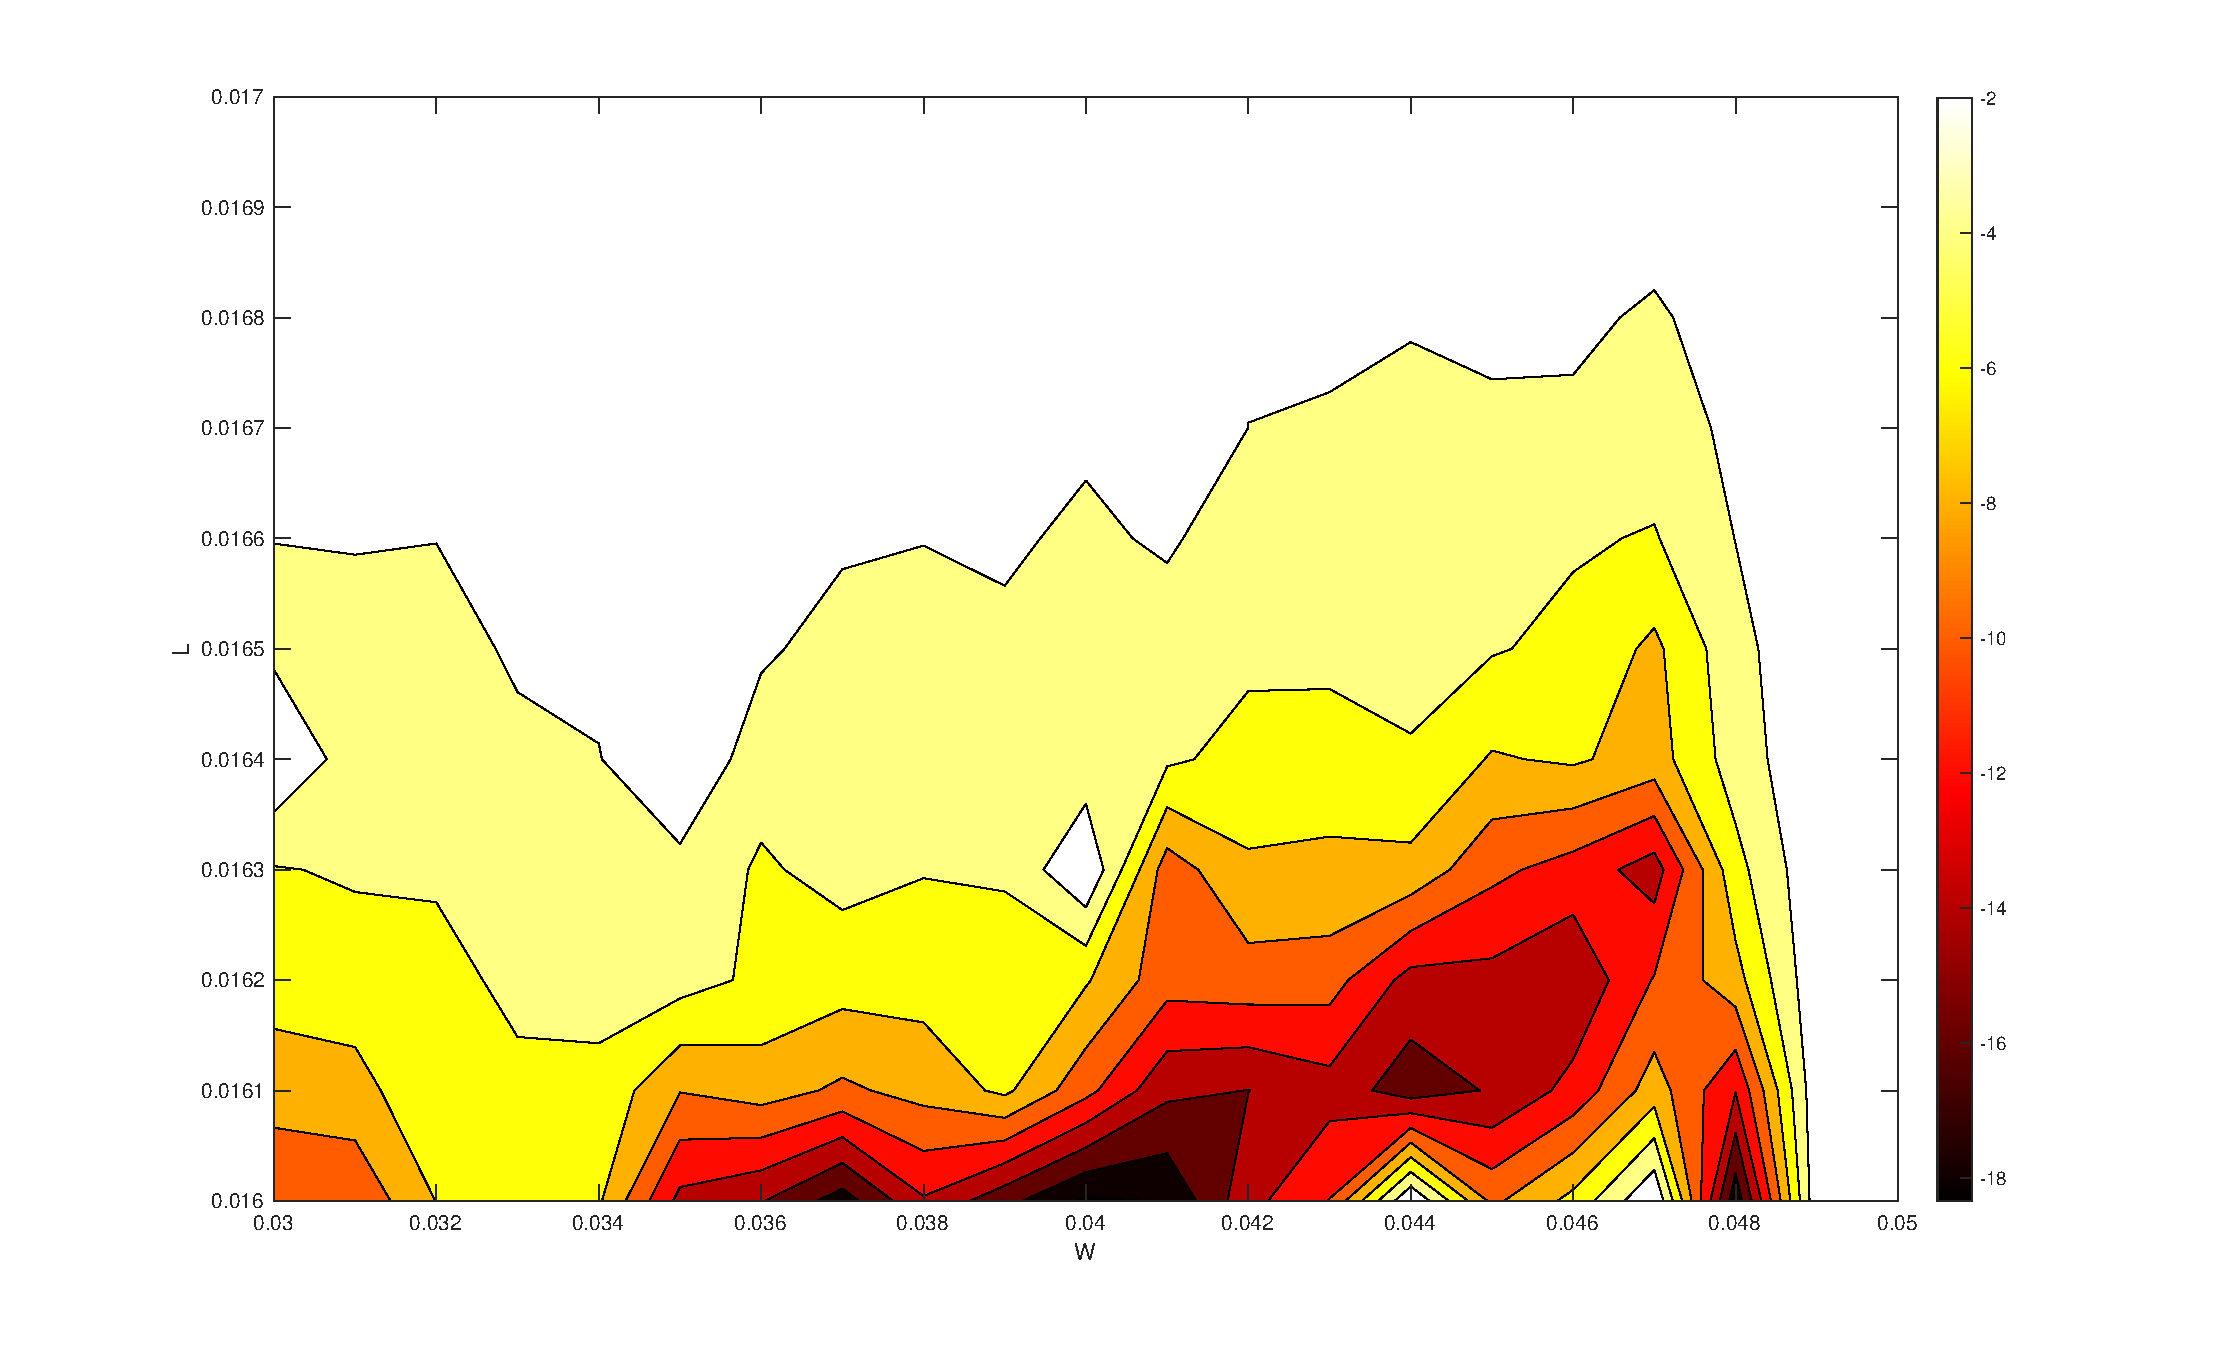
\includegraphics[scale=0.25]{First_Contour_LOG.pdf}
		\caption{}
		\label{fig:first contour}
	\end{subfigure}
	\hfill
	\begin{subfigure}{0.48\linewidth}
		\def\svgwidth{\linewidth}
		\tiny{\input{Second_Contour_LOG_2_tex.pdf_tex}}
		%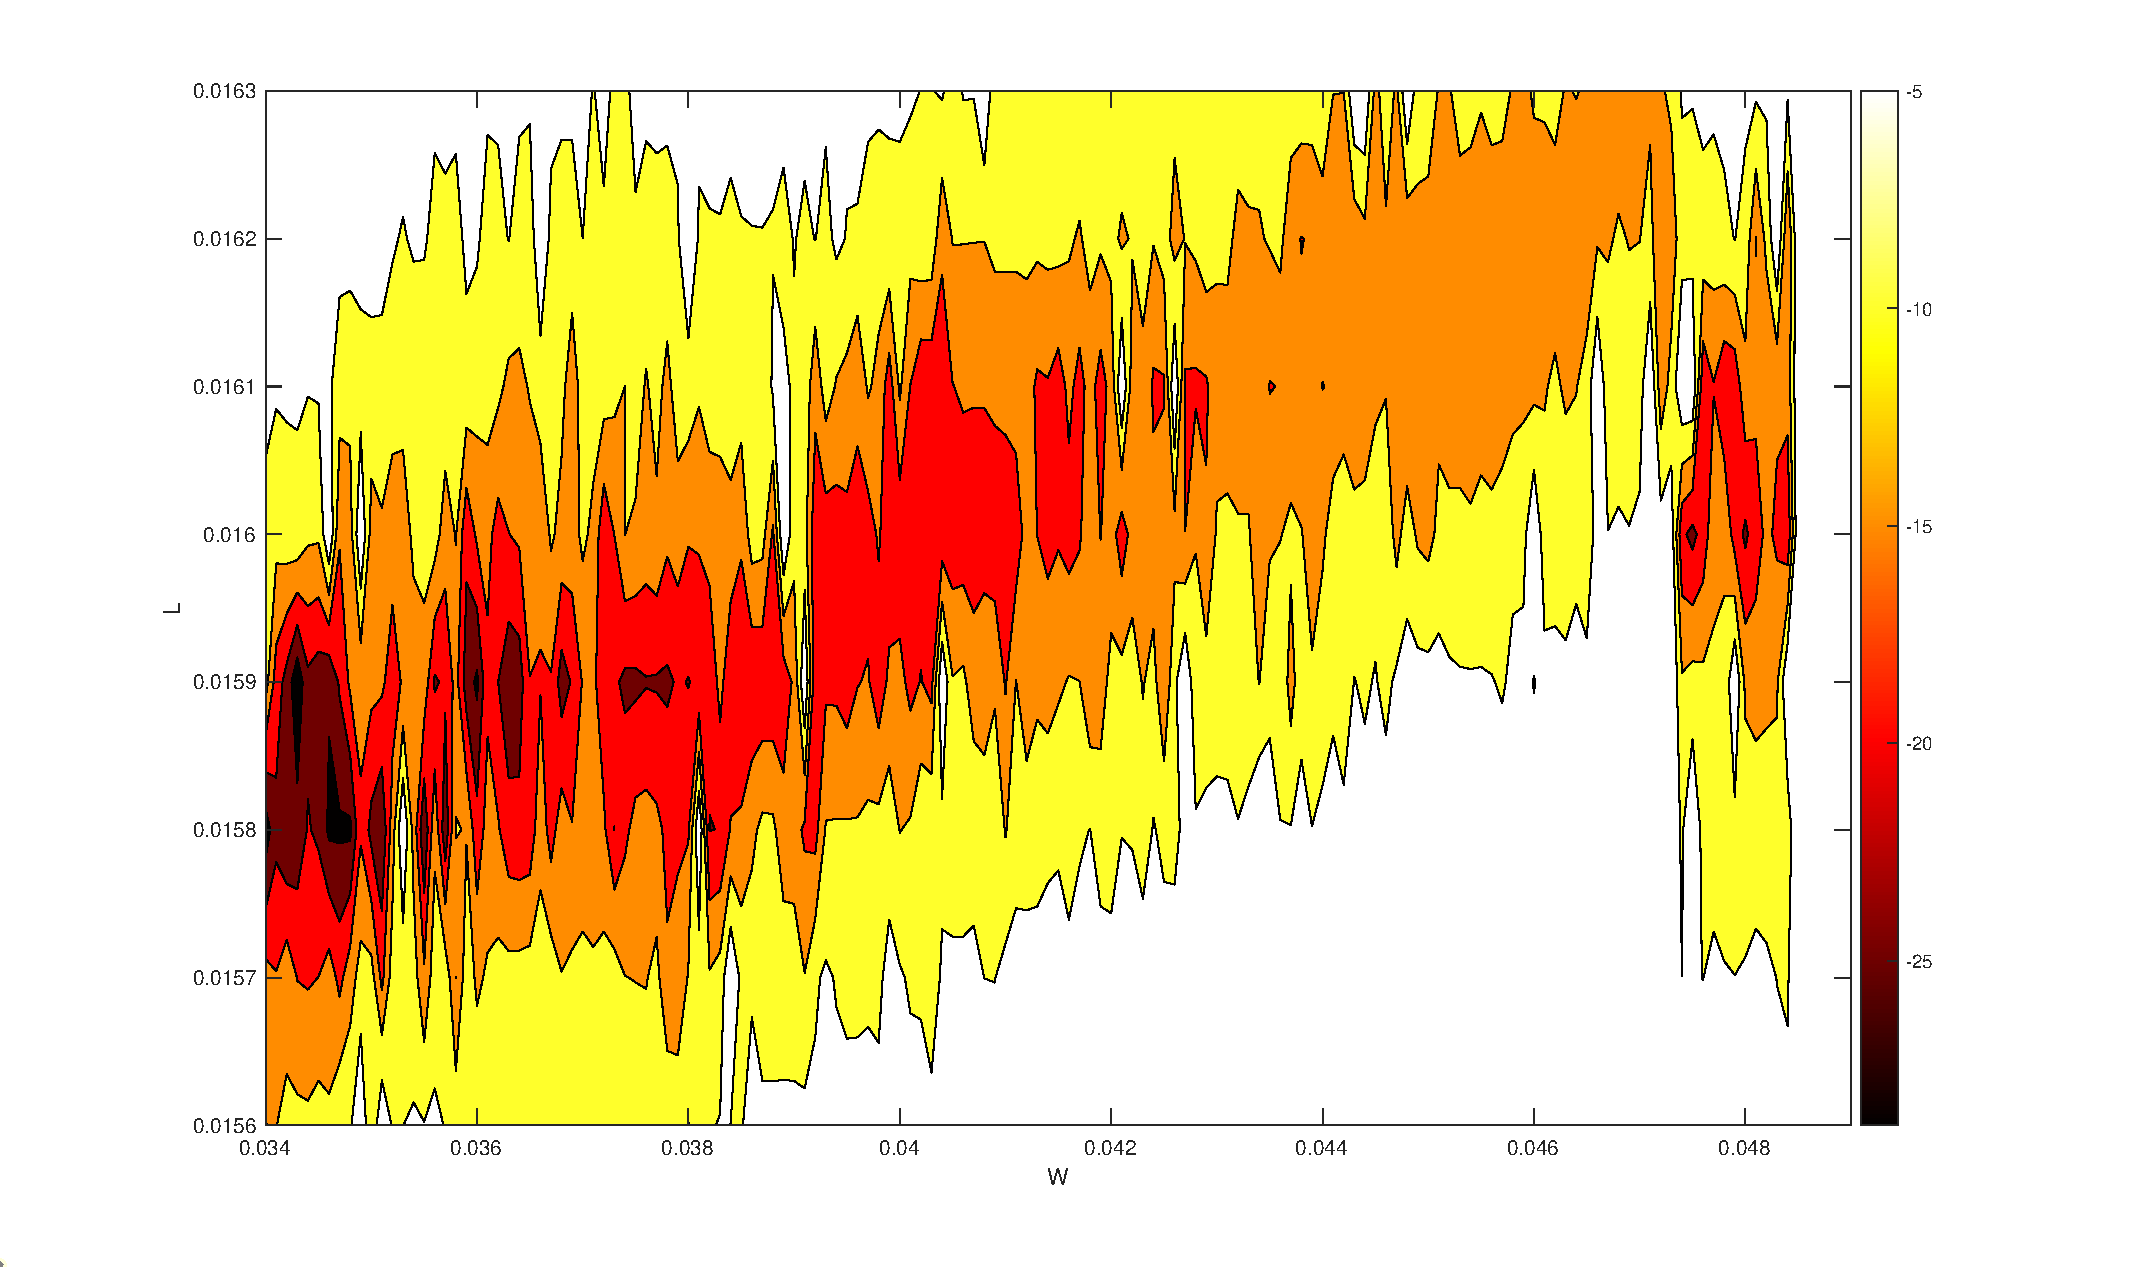
\includegraphics[scale=0.25]{Second_Contour_LOG.pdf}
		\caption{}
		\label{fig:second contour}
	\end{subfigure}
	\caption{First (a) and second (b) contour plots depending on the patch size ($L_{patch}$ and $W_{patch}$ variations)}
\end{figure*}

\begin{figure}
	\begin{center}
		\begin{subfigure}{0.5\linewidth}
			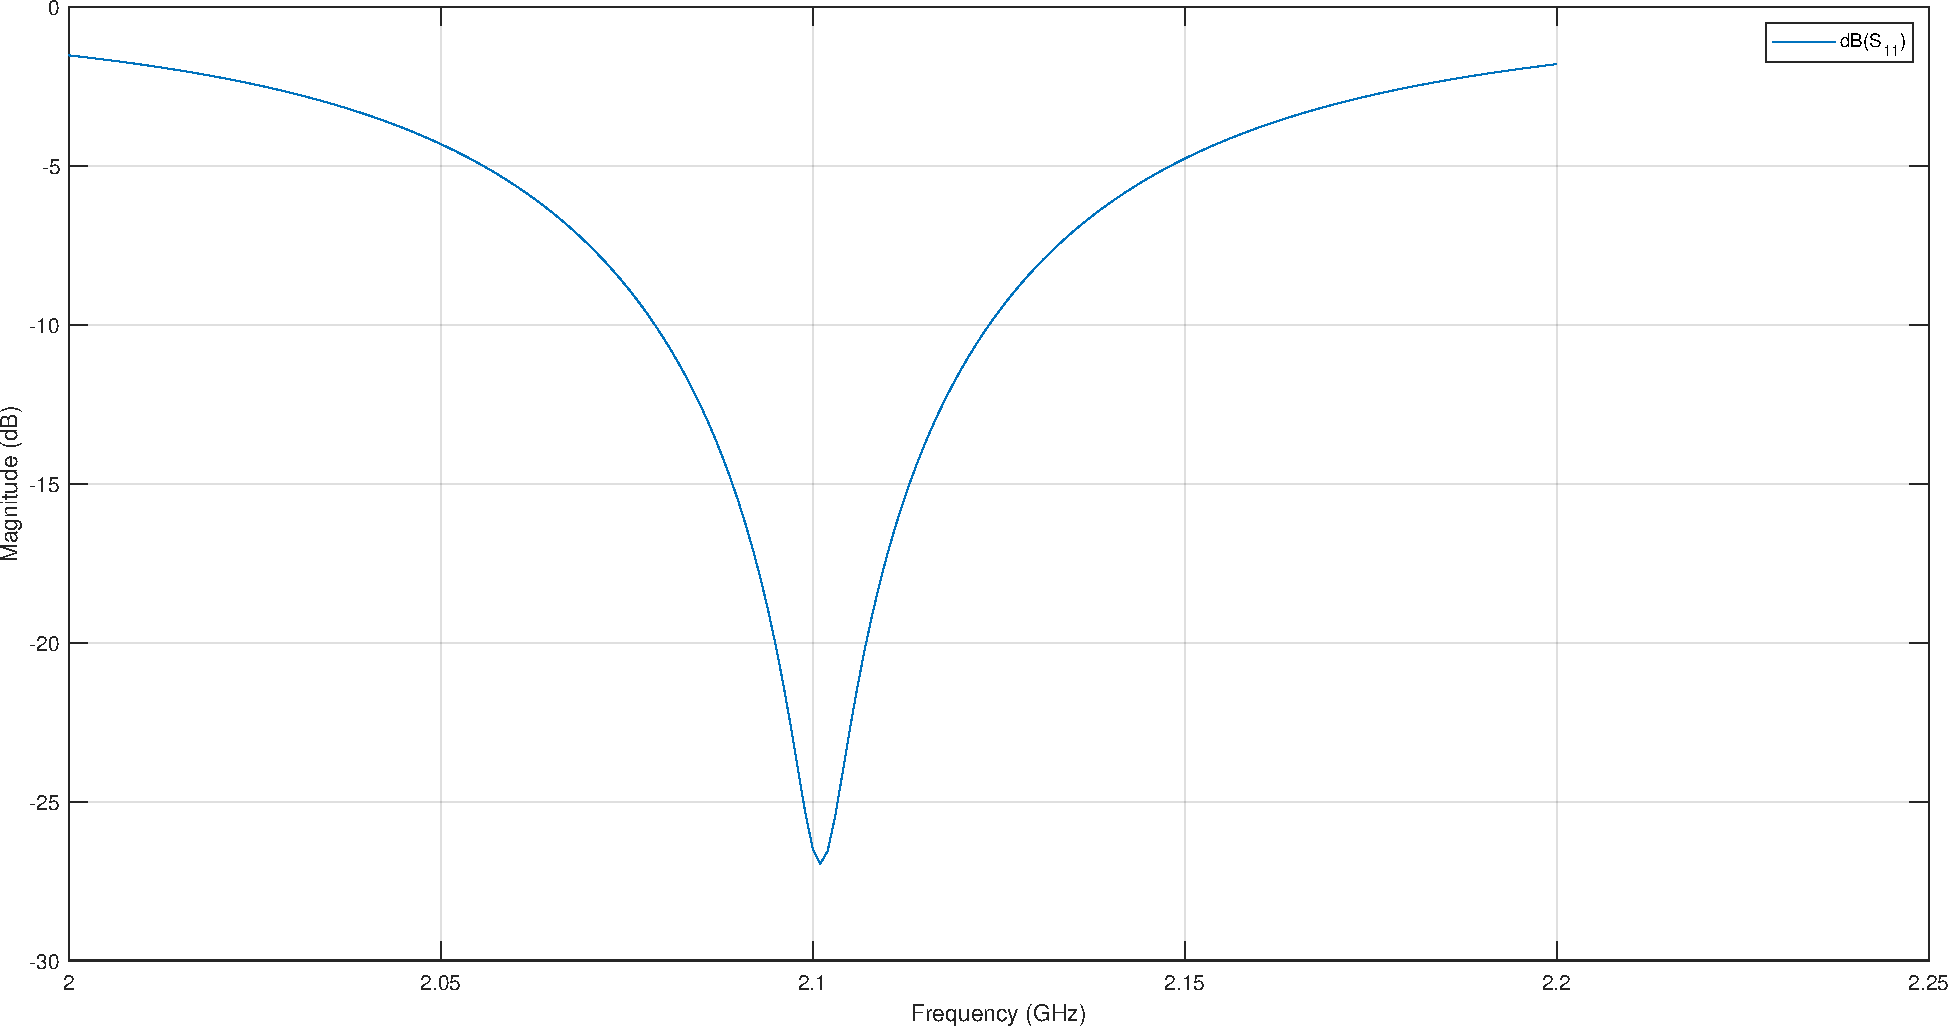
\includegraphics[scale=0.25]{gamma1.pdf}
		\end{subfigure}
		\begin{subfigure}{0.5\linewidth}
		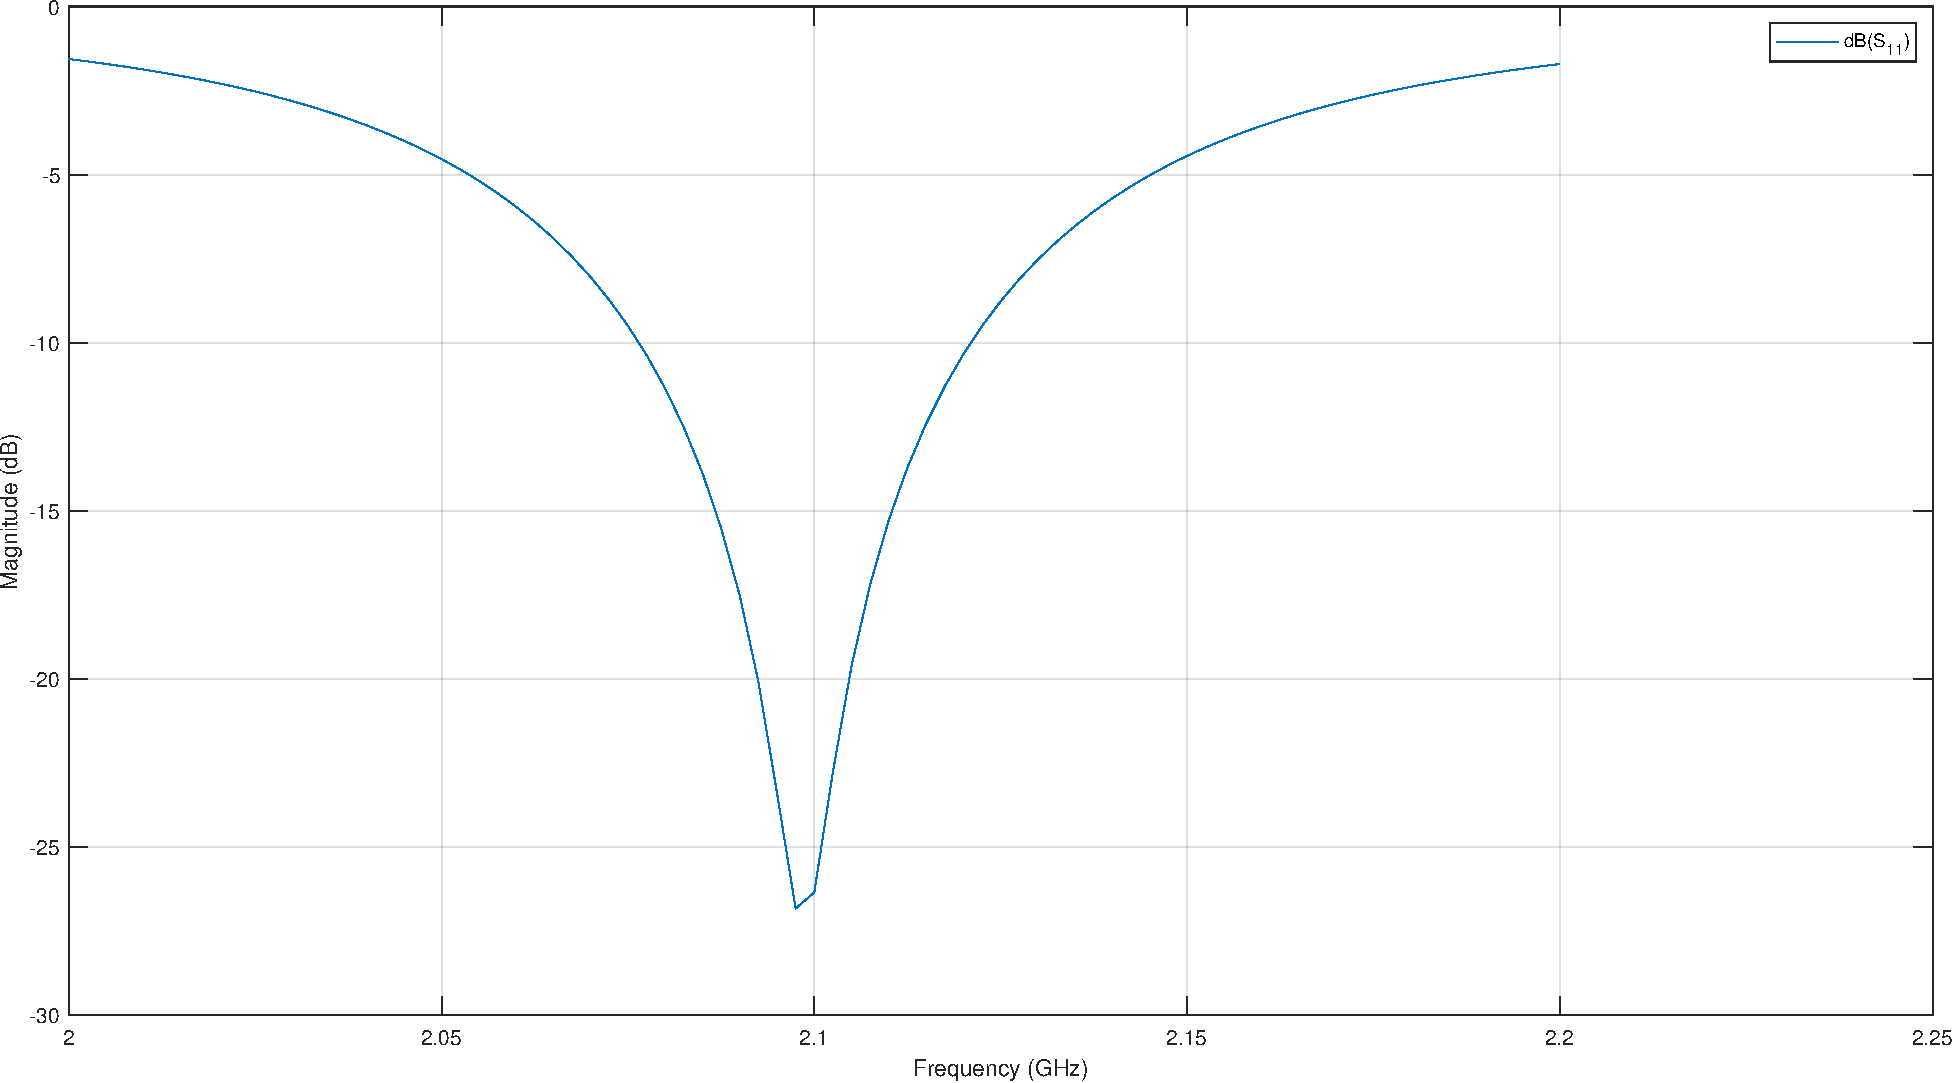
\includegraphics[scale=0.25]{gamma3.pdf}
	\end{subfigure}
	\caption{\fontfamily{lmss}\selectfont
	\color{gray}The two best $\Gamma$ plots depending on the specific patch size expressed coupled variations ($L_{patch},W_{patch}$) and represented in a frequency range of $[2.0,2.1]\,GHz$}
\label{fig:Gamma couple LpWp}
	\end{center}  
\end{figure}
\begin{figure}[h]
	\begin{center}
		\begin{subfigure}{0.5\linewidth}
			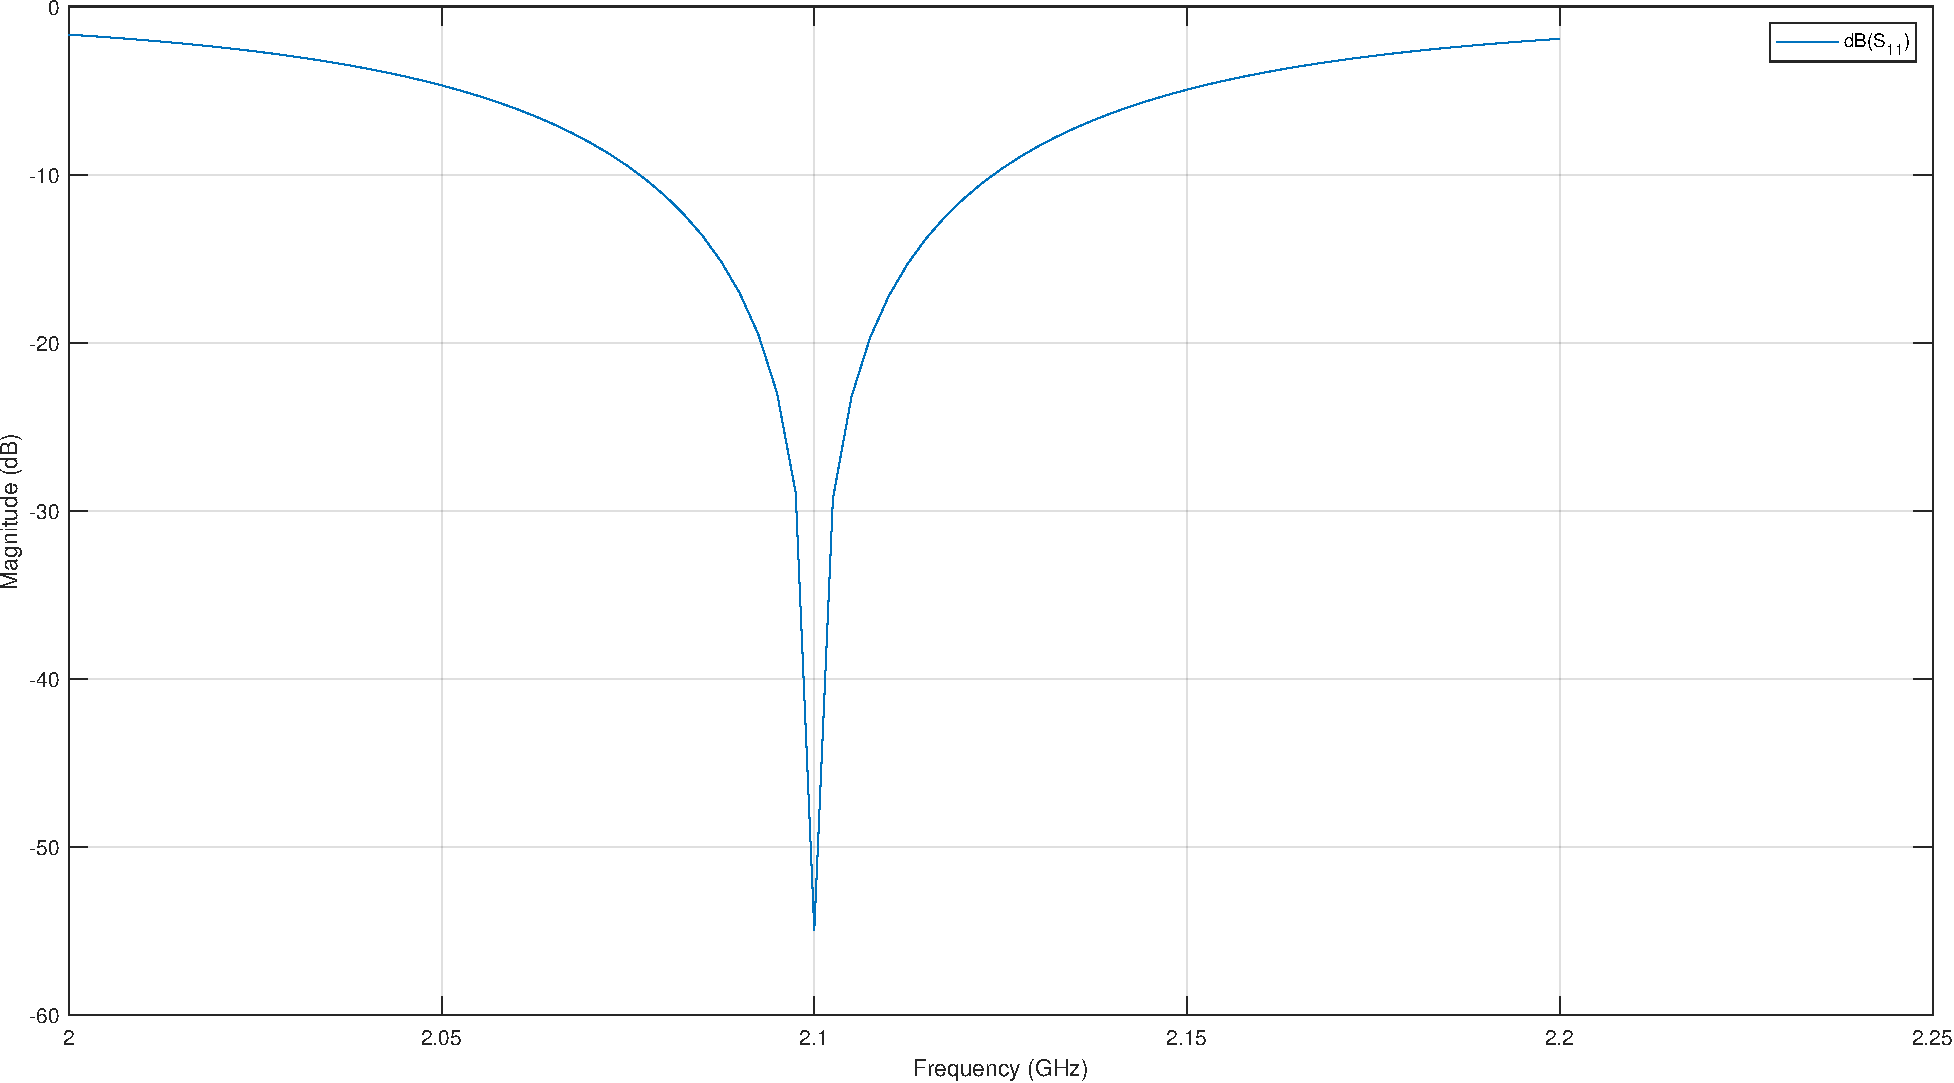
\includegraphics[scale=0.25]{gamma_wfeed.pdf}
		\end{subfigure}
		\begin{subfigure}{0.5\linewidth}
			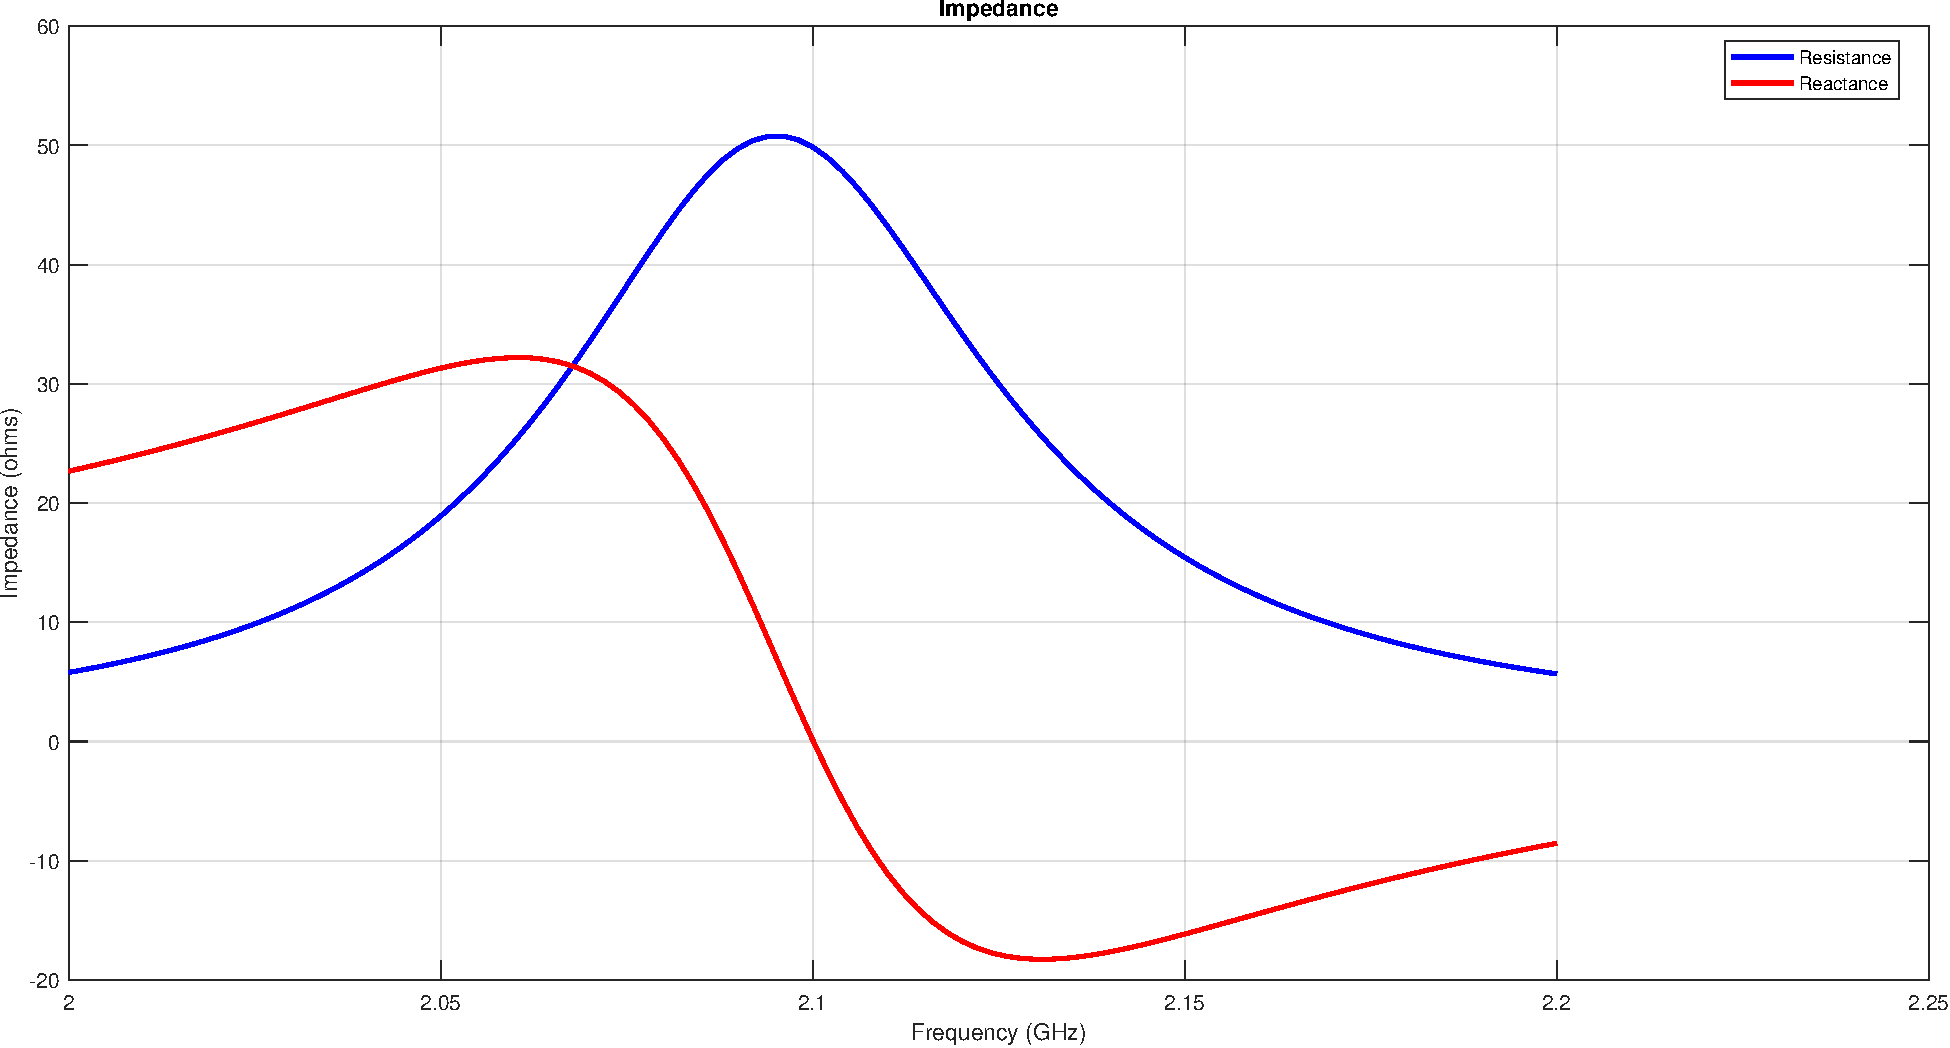
\includegraphics[scale=0.25]{matching_wfeed.pdf}
		\end{subfigure}
		\caption{\fontfamily{lmss}\selectfont
		\color{gray}
	Final $\Gamma$ and impedance matching plots after further refinement including $w_{feed}$ change}
\label{fig:Gamma and Z}
	\end{center}  
\end{figure}
\begin{figure}[h]
	\begin{center}
		\begin{subfigure}{0.5\linewidth}
			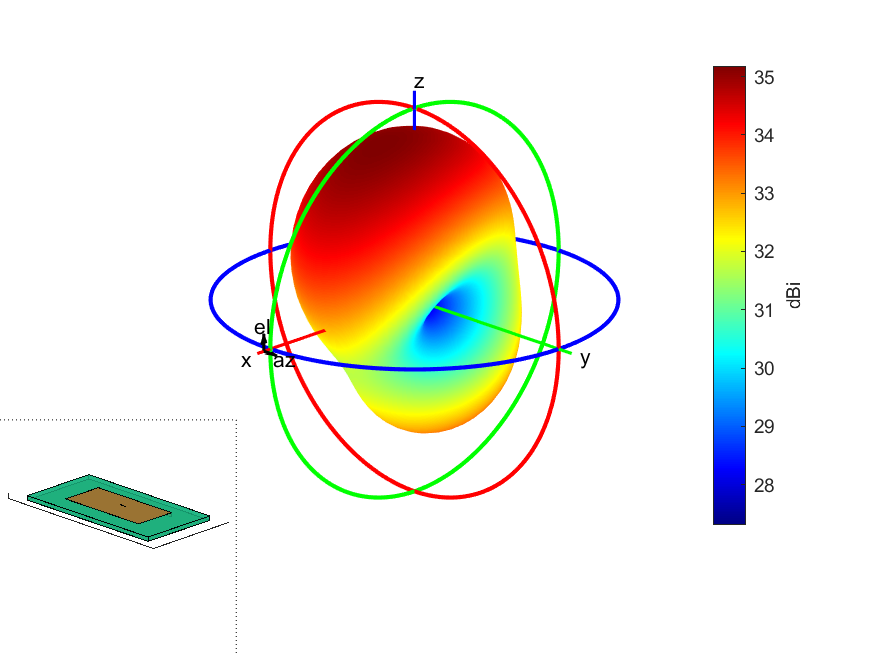
\includegraphics[scale=0.5]{gain_3D_pifa.pdf}
			\caption{}
		\end{subfigure}
		\begin{subfigure}{0.5\linewidth}
			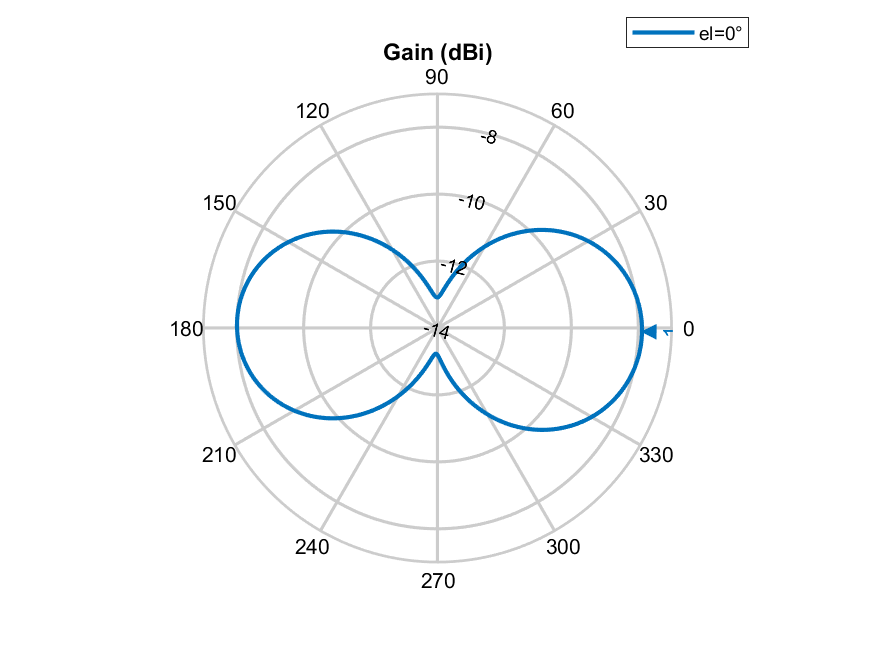
\includegraphics[scale=0.5]{gain_azimuth_pifa.pdf}
		\caption{}	\end{subfigure}
		\begin{subfigure}{0.5\linewidth}
		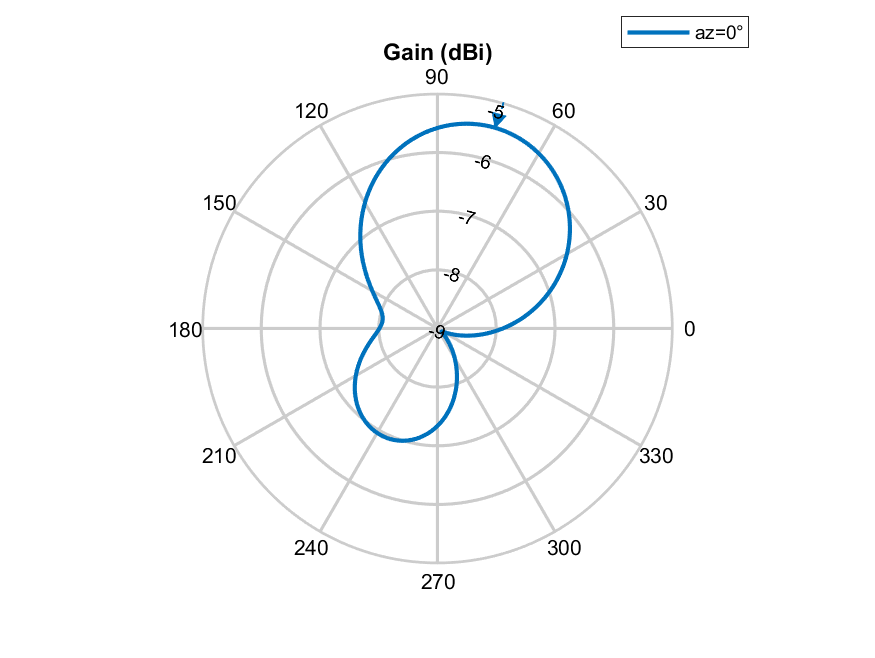
\includegraphics[scale=0.5]{gain_elevation_pifa.pdf}
	\caption{}	\end{subfigure}
	\begin{subfigure}{0.5\linewidth}
	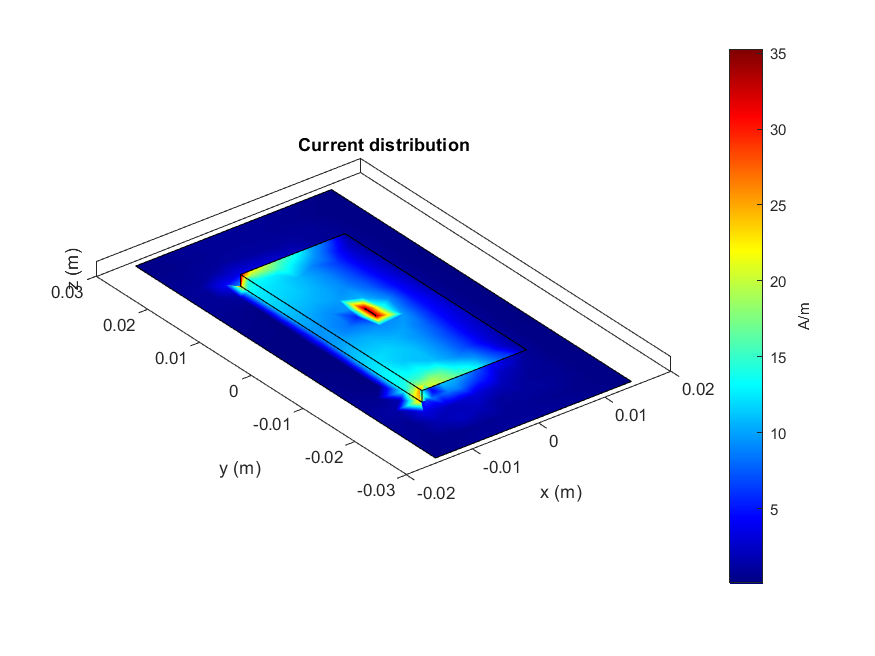
\includegraphics[scale=0.5]{pifa_currents.pdf}
	\caption{} \end{subfigure}
		\caption{\fontfamily{lmss}\selectfont
			\color{gray}
		Gain patterns (a) in 3D, (b) in the nulle elevation plane, (c) in the null azimuth plane and (d) 3D current plot on the patch antenna }
	\end{center}  
\end{figure}
%%% le seguenti 3 figure le faremo più grandi una volta che sapremo dove effettivamente saranno posizionate nella relazione finale %%% 
%% w_{feed} = 0.001 
\begin{center}
	\begin{figure}[h]
		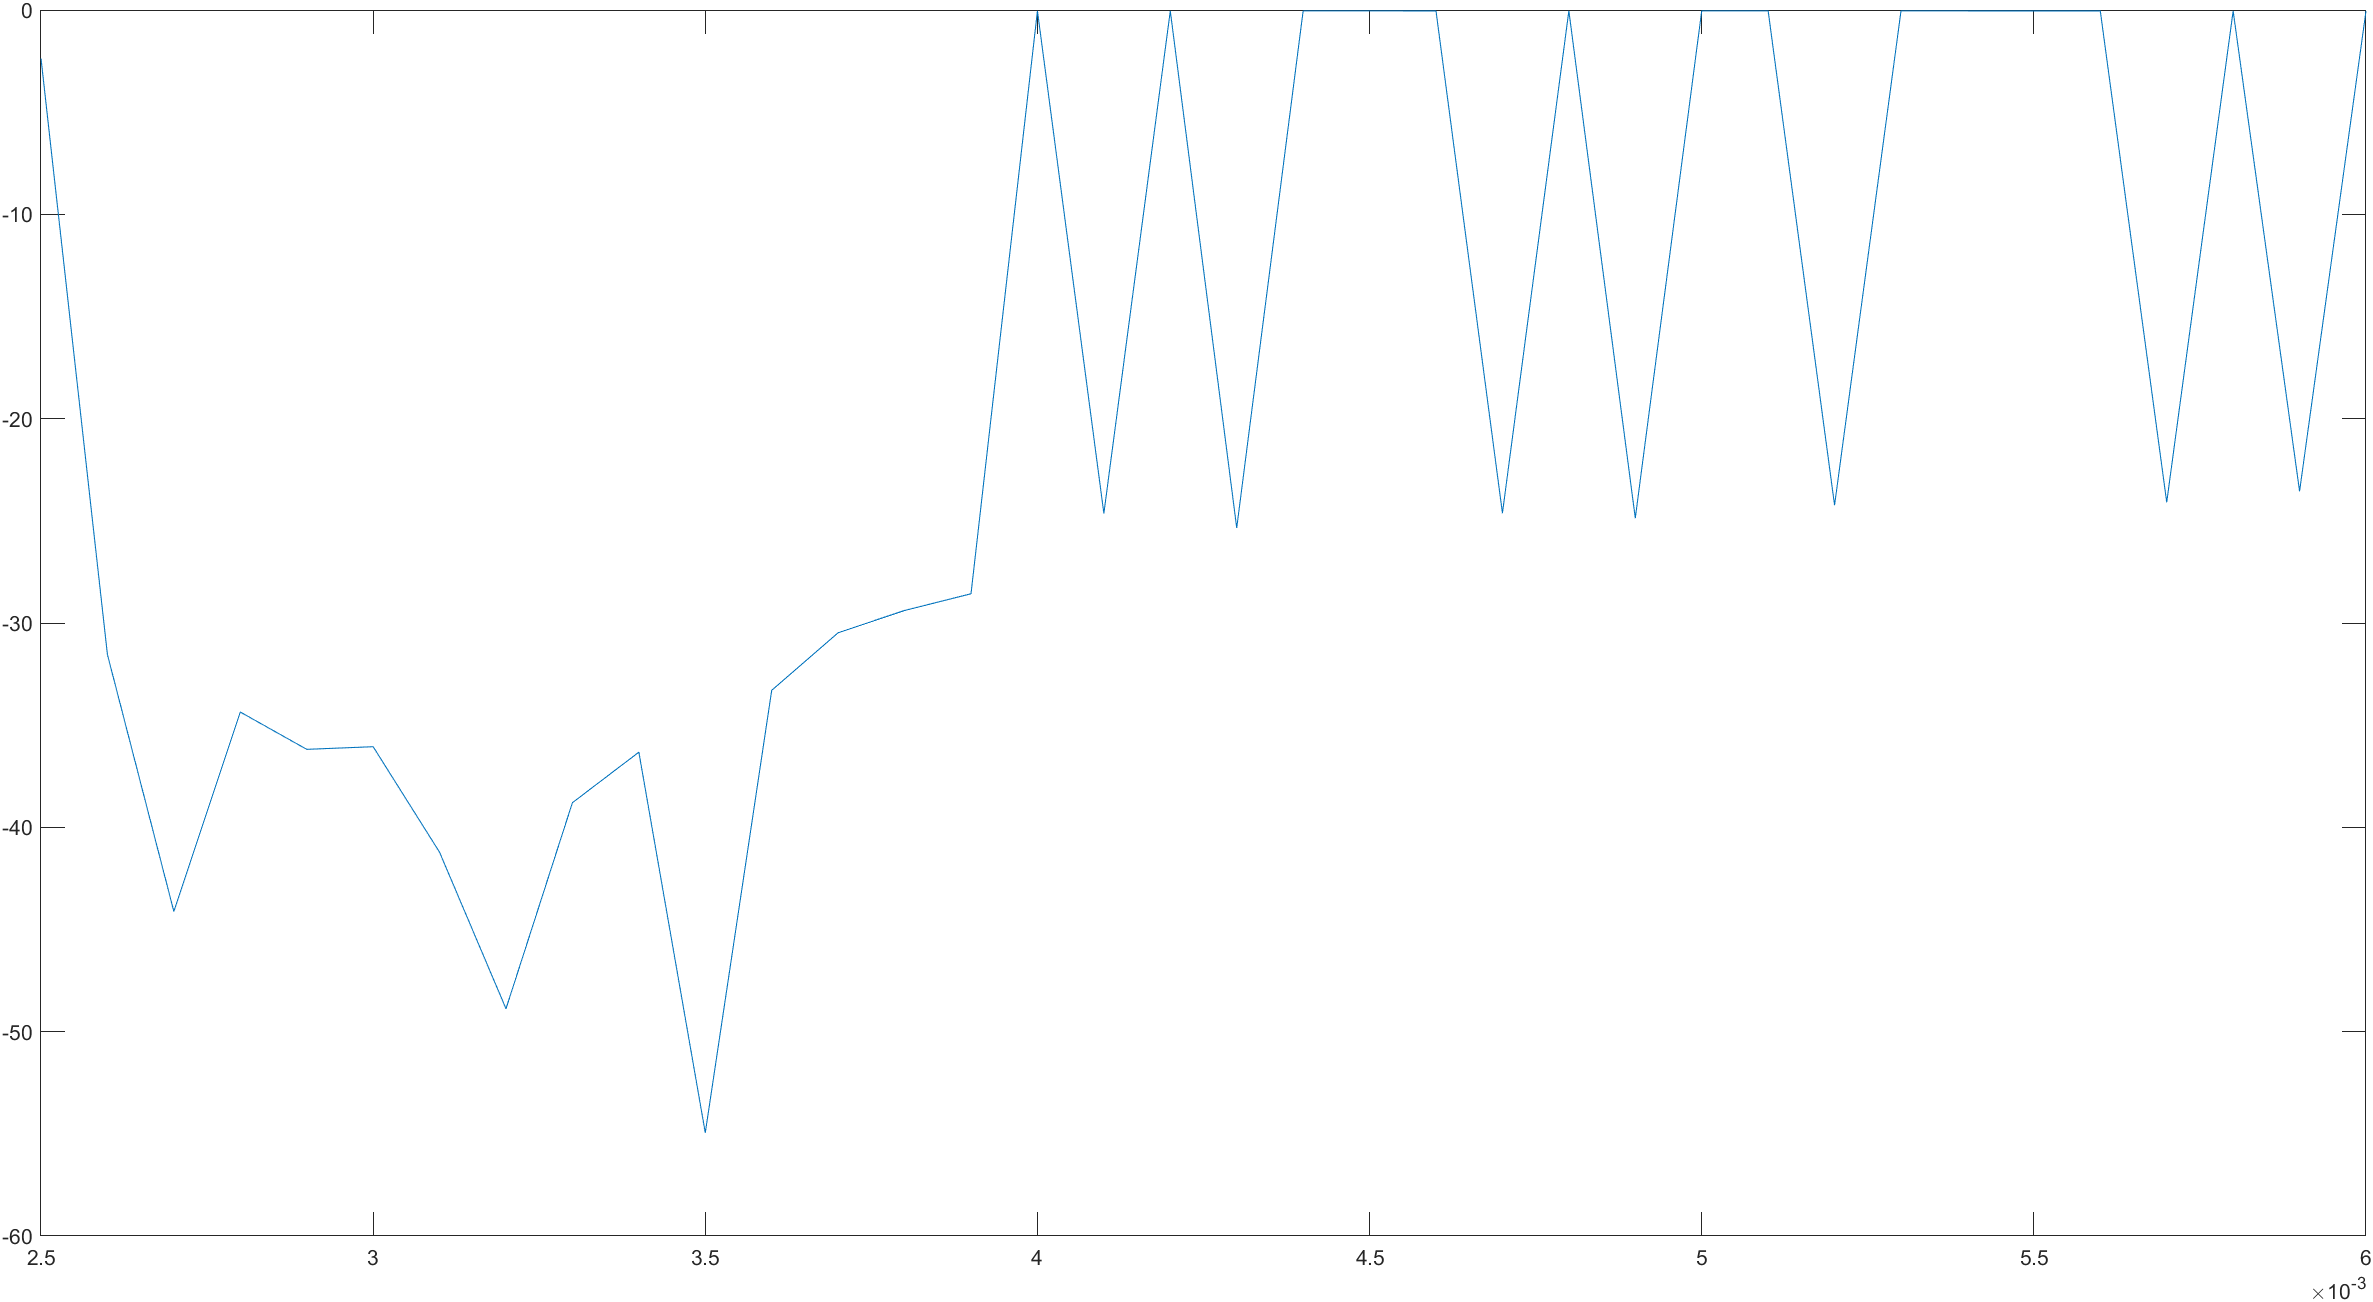
\includegraphics[scale=0.3]{mesh_levels.png}
		\caption{{Minimum of the reflection coefficient $\Gamma\, [dB]$ in the frequency range $2.0\div 2.2\,GHz$ depending on the varying mesh density level}}
	\end{figure}
\end{center}
\begin{center}
\begin{figure}
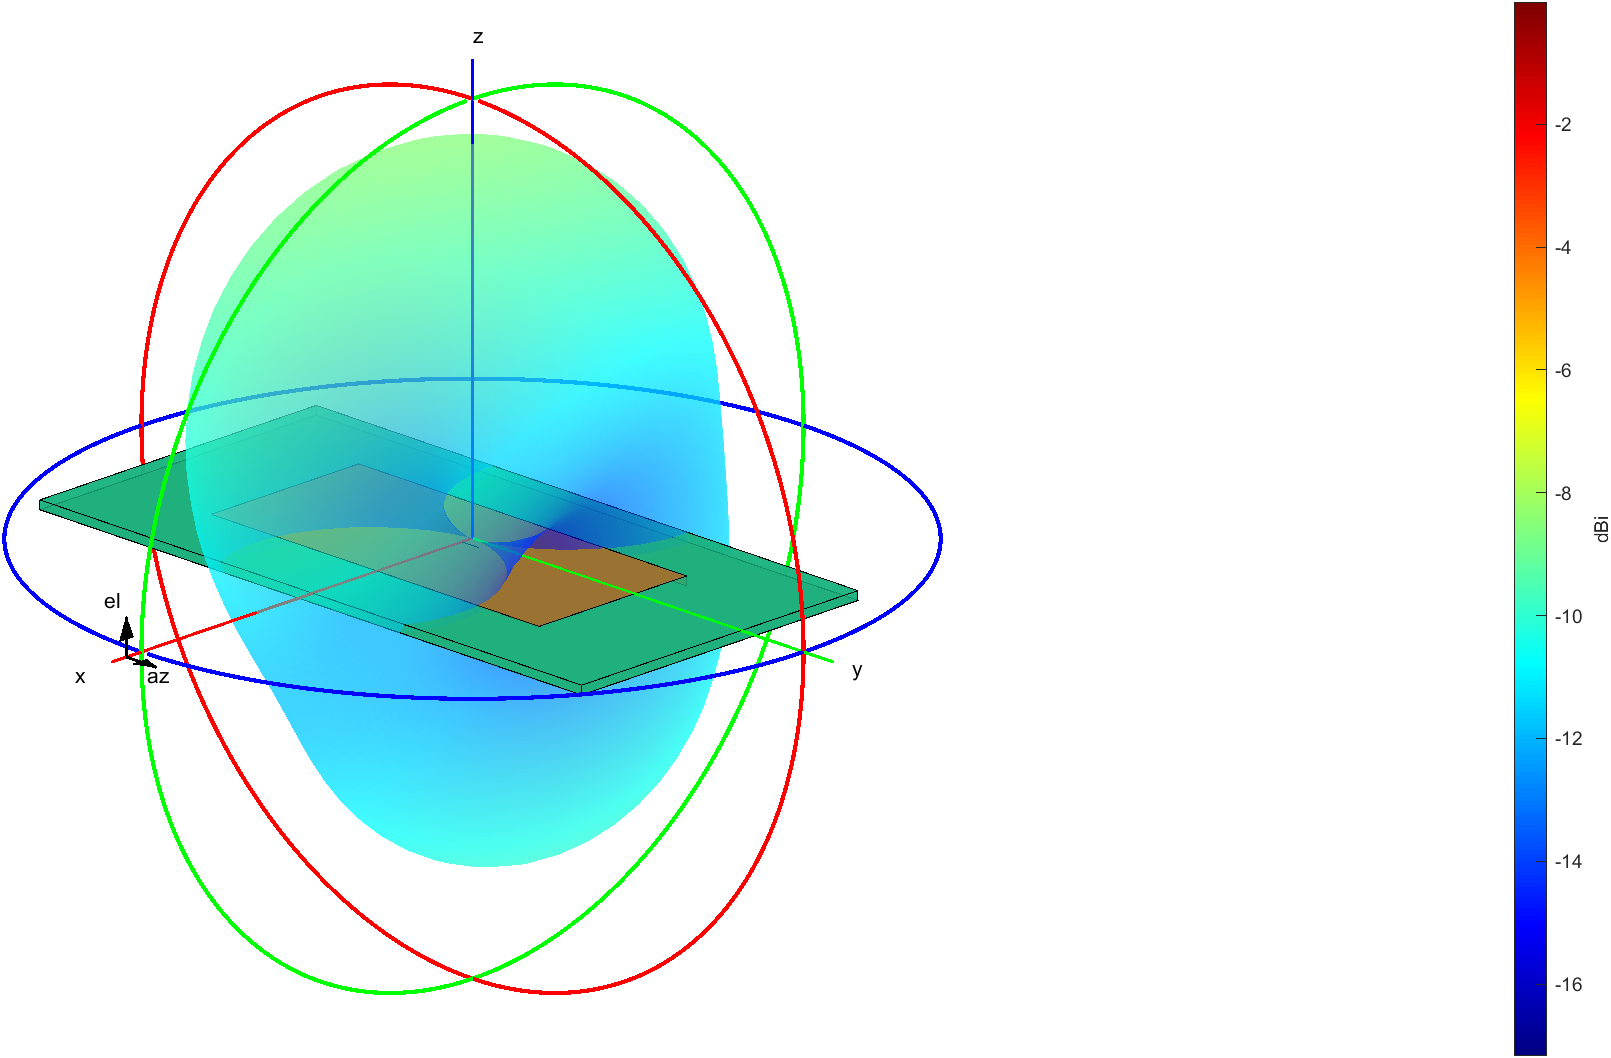
\includegraphics[width = 0.3\linewidth]{gain_patch.png}
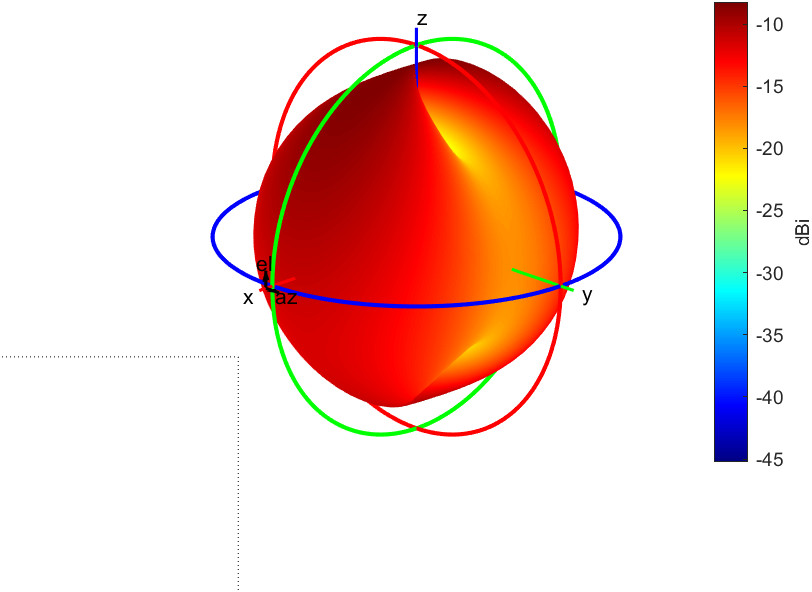
\includegraphics[width = 0.3\linewidth]{gain_patch_v.png}
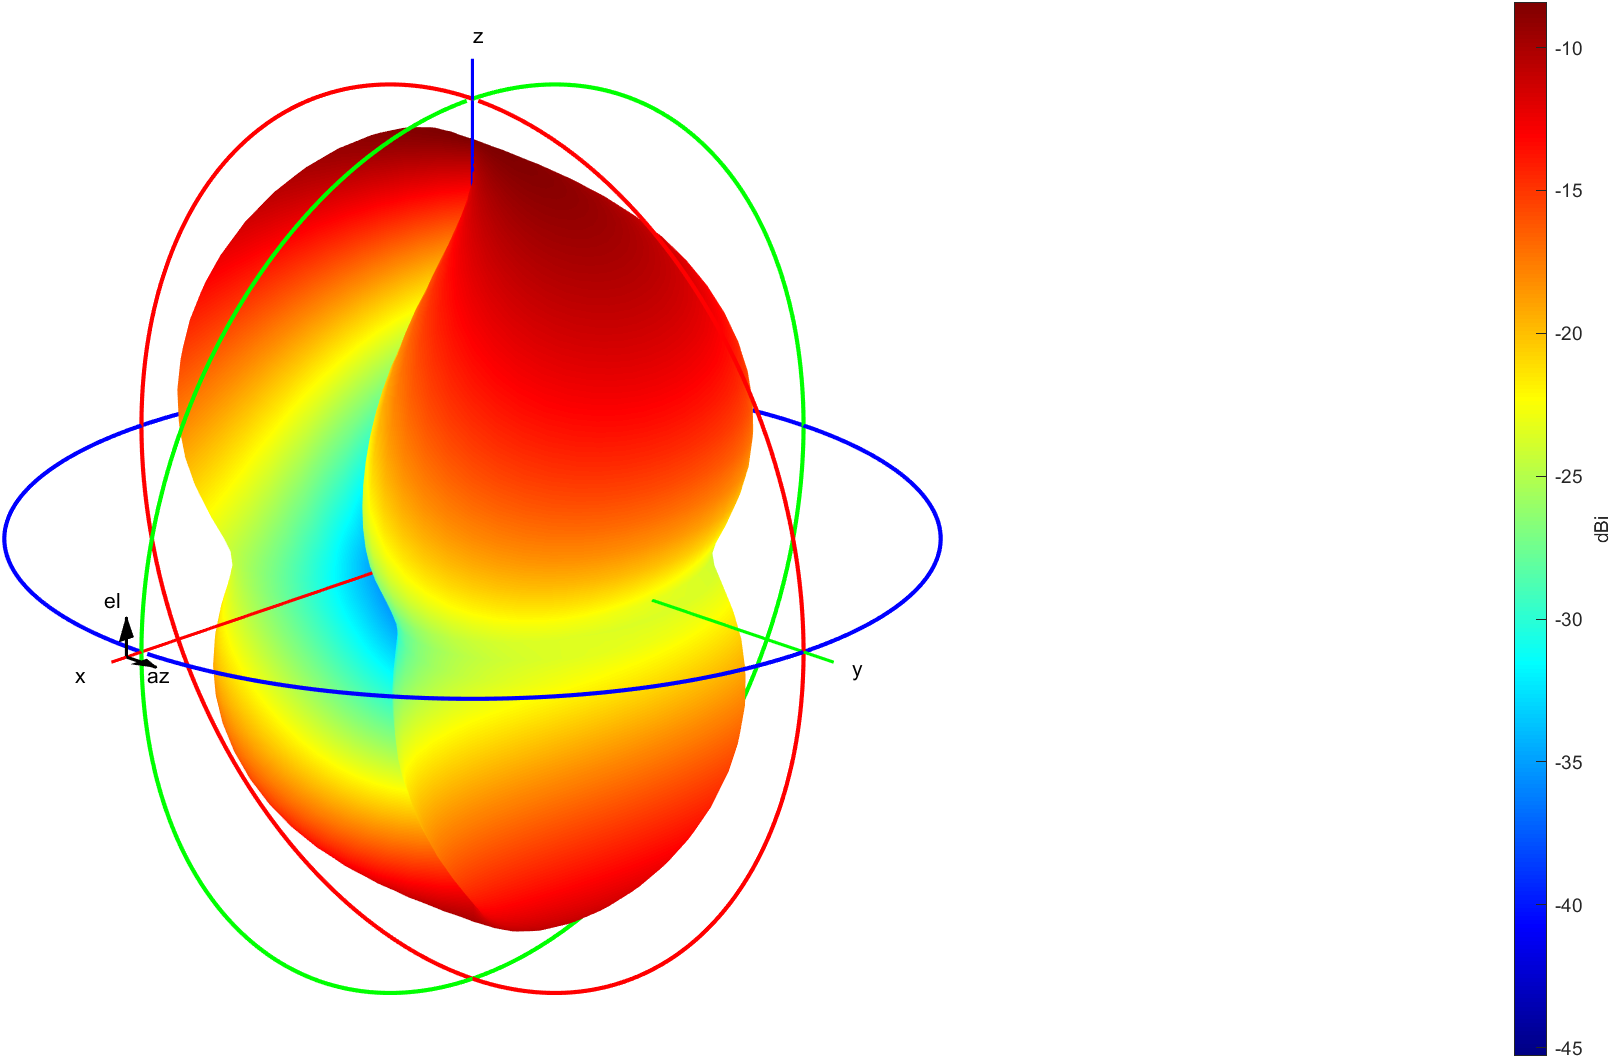
\includegraphics[width = 0.3\linewidth]{gain_patch_h.png}
\caption{Gain pattern (left), gain pattern with vertical polarization (center) and with the horizontal one (right)}
\end{figure}
\end{center}
	\paragraph{\fontfamily{qag}\selectfont\color{Turquoise}From the PIFA to a PCB stack approximation}
Since the \texttt{\color{Mahogany}Antenna Array Designer} is not able to generate an array of PIFAs , the \texttt{\color{Mahogany}Sensor Array Analyzer} has been used to create that type of structure, starting from the Tchebyshev array factor design made in the first part and from the previous optimization process of a single PIFA. In the last part the overall array of PIFAs needs to be analyzed by means of beamsteering for particular angles, total gain, electric and magnetic field patterns. Unfortunately, not all of this information can be extracted by using uniquely the the \texttt{\color{Mahogany}Sensor Array Analyzer} tool. This fact led to the use of another tool, the \texttt{\color{Mahogany}PCB Antenna Designer}, so that all the parameters required for the project could be analyzed. With this last tool, a similar structure to that of the PIFA has been realized and introduced as the antenna element of the array distribution. Just before moving to the array analysis, a comparison between the single antenna being a PIFA structure and the antenna created by using a PCB stack was performed. A single limitation in the use of the \texttt{\color{Mahogany}PCB Antenna Designer} has been encountered, but it has been overcome with an approximation strategy. Thus, the PIFA and the PCB stack designed are not perfectly identical, but their single and overall performance inside the array had shown a slight quantifiable difference. The limitation consisted in the absence of a specific option or combination of commands that would allow to realize the rectangular shorting pin between the patch and the ground. The only thing the designer can do is to replace this kind of shorting pin with a series of small diameter (e.g. $0.4\,mm$) cylindrical shorting pins (see \textbf{\cref{fig:pcb shorting}}) close to one edge of the patch, across the patch width direction. With this design choice, a very similar behaviour to that of the PIFA structure was possible to simulate. To support this results, a comparison of the 2D gain patterns (elevation and azymuth cut) of the PIFA to those of the PCB stack antenna has been realized in terms of the mean square error values, shorten $MSE$, related to the two specific two-dimensional patterns considered ($MSE_{el}$ in the elevation cut directivity pattern and $MSE_{az}$ in the azimuth cut directivity pattern). Furthermore, since the \texttt{\color{Mahogany}Sensor Array Analyzer} allows the plotting of some patterns such as the directivity (but not of the gain), a comparison between the 2D patterns of the antenna array of PIFAs and the array of PCBs has been presented. In that case the error is presented as a comparison between the main lobe levels in the PIFA array and the PCB array cases, but also in terms of a first side lobe levels of the two arrays. This discussion was necessary, because moving to the last part of the project required a deeper study of the array of antennas, that will be displayed by using the PCB antenna as the element of the array. 

\begin{table}
	\begin{center}
		{\fontfamily{lmss}\selectfont	\begin{tabular}{||m{1.8cm}|m{3.6cm}|m{3.6cm}|m{3.6cm}|m{3.6cm}||}
				\hline
				\textbf{Direction} & \textbf{$D_{ML,az}$ error} & \textbf{$D_{SL,az}$} & \textbf{$D_{ML,el}$ error} & \textbf{$D_{SL,el}$} \\
				\hline 
		Broadside ($90^\circ$) & \begin{subtable}{1.8cm} 
			\begin{tabular}{|l|l|}
				\hline
				$\Delta D_{ML}$ & $\Delta D_{ML}^r$\%  \\
				\hline
				$2.39\,dB$ & $3.3\,\%$ \\
					\hline
			\end{tabular} 
			\end{subtable} & \begin{subtable}{1.8cm} 
			\begin{tabular}{|l|l|}
					\hline
				$\Delta D_{SL}$ & $\Delta D_{SL}^r$\% \\
				\hline
				$0.96\,dB$ & $2.7\,\%$ \\
					\hline
			\end{tabular} 
		\end{subtable} & \begin{subtable}{1.8cm} 
		\begin{tabular}{|l|l|}
				\hline
			$\Delta D_{ML}$ & $\Delta D_{ML}^r$\% \\
			\hline
			$0.81\,dB$ & $1.1\,\%$ \\
				\hline
		\end{tabular} 
	\end{subtable} & \begin{subtable}{1.8cm} 
	\begin{tabular}{|l|l|}
			\hline
		$\Delta D_{SL}$ & $\Delta D_{SL}^r$\% \\
		\hline
		$0.35\,dB$ & $1.6\,\%$ \\
			\hline
	\end{tabular} 
\end{subtable} \\
\hline

%%%%%%%%%%%%%%%%%%%%%%%%%%%%55
%%%%%%%%%%%%%%%%%%%%%%%%%%%%%
%%%%%%%%%%%%%%%%%%%%%%%%%%%%

%%%%%%%%%%%%%%%%%%%%%%%%%%%%55
%%%%%%%%%%%%%%%%%%%%%%%%%%%%%
%%%%%%%%%%%%%%%%%%%%%%%%%%%%
			\hline 
Off Boresight ($45^\circ$) & \begin{subtable}{1.8cm}\begin{tabular}{|l|l|}
			\hline
		$\Delta D_{ML}$ & $\Delta D_{ML}^r$\% \\
		\hline
		$0.05\,dB$ & $0.07\,\%$ \\
			\hline
	\end{tabular} 
\end{subtable} & \begin{subtable}{1.8cm} 
	\begin{tabular}{|l|l|}
			\hline
		$\Delta D_{SL}$ & $\Delta D_{SL}^r$\% \\
		\hline
		$1.37\,dB$ & $3.4\,\%$ \\
			\hline
	\end{tabular} 
\end{subtable} & \begin{subtable}{1.8cm} 
	\begin{tabular}{|l|l|}
			\hline
		$\Delta D_{ML}$ & $\Delta D_{ML}^r$\% \\
		\hline
		$0.03\,dB$ & $0.04\,\%$ \\
			\hline
	\end{tabular} 
\end{subtable} & \begin{subtable}{1.8cm} 
	\begin{tabular}{|l|l|}
			\hline
		$\Delta D_{SL}$ & $\Delta D_{SL}^r$\% \\
		\hline
		$4.1\,dB$ & $1.4\,\%$ \\
			\hline
	\end{tabular} 
\end{subtable} \\
\hline
		\end{tabular}}
		\caption{Comparison between the array of PIFAs and the array of PCBs in terms of the directivity evaluated in their main lobes and first side lobes, both in the broadside and $45^\circ$ off the boresight direction, both in the azimuth cut ($az$) and elevation cut ($el$) planes. The comparison has been made in terms of the directivity difference ($\Delta D_{\#}=D_{PIFAs}-D_{PCBs}$ in $dB$) in the corresponding positions and also as a relative percentage error ($\Delta D^r_{\#}$\%, the ratio between $\Delta D_{\#}$ and the directivity in the array of PIFAs case ($D_{PIFAs}$)}
		\label{table:array comparison error}
	\end{center}
\end{table}
%%%%%%%%%%%%%%%%%%%%%%%%%%%%%%%%%%%%%%%%%%%%%%%%%%%%%%%%%
%%%%%%%%%%%%%%%%%%%%%%%%%%%%%%%%%%%%%%%%%%%%%%%%%%%%%%%%%
%%% creare una tabella  %%%%%%%%%%%%%%%%%%%%%%%%%%%%%%%%%
%%% in cui inserire i corretti dati di confronto %%%%%%%%
%%% inseriti in una tabella dopo che comincia %%%%%%%%%%%
%%% "Overall patch antenna array performante" %%%%%%%%%%%
%%%%%%%%%%%%%%%%%%%%%%%%%%%%%%%%%%%%%%%%%%%%%%%%%%%%%%%%%
%%%%%%%%%%%%%%%%%%%%%%%%%%%%%%%%%%%%%%%%%%%%%%%%%%%%%%%%%
\begin{table}
	\begin{center}
		{\fontfamily{lmss}\selectfont	\begin{tabular}{||m{1.8cm}|m{2.6cm}|m{2.6cm}|m{2.6cm}|m{2.6cm}|m{2.6cm}||}
				\hline
				*** & Position & $E$-field ($90^\circ$) & $H$-field ($90^\circ$) & $E$-field ($45^\circ$) & $45$-field ($90^\circ$) \\
						\hline 
			$PCB_{-2}$ & $(0,-2d_{opt},z_{fre})$ & $0.1027$ & $0.0139$ & $0.2071$ & $0.0269$ \\ 
			\hline
				$PCB_{-1}$ & $(0,-d_{opt},z_{fre})$ & $0.2923$ & $0.0377$ & $0.1889$ & $0.0100$ \\
				\hline
				$PCB_0$ & $(0,0,z_{fre})$& $0.4189$& $0.0522$& $0.2422$ & $0.0174$ \\
				\hline 
				$PCB_1$ & $(0,d_{opt},z_{fre})$ & $0.3306$ & $0.0367$ & $0.2619$ & $0.0215$ \\
				\hline 
				$PCB_2$ & $(0,2d_{opt},z_{fre})$ & $0.1350$ & $0.0143$ & $0.2922$ & $0.0270$ \\ 
				\hline
			\end{tabular}}
		\caption{Particular electric ($E$) and magnetic ($H$) field values measured in both broadside ($90^\circ$) and in the $45^\circ$ off the boresight directions. The $E$-field is measured in $\left[\frac{V}{m}\right]$ while the $H$-field in $\left[\frac{A}{m}\right]$. The fields have been measured with respect to the centers of each element antenna vertically off the array plane at a height distance of $z_{fresnel}$, the limit of the radiative, near field region, in a global reference system.}
		\label{table:EH fields}
		\end{center}
	\end{table} 
\begin{center}
	\begin{figure}[h]
		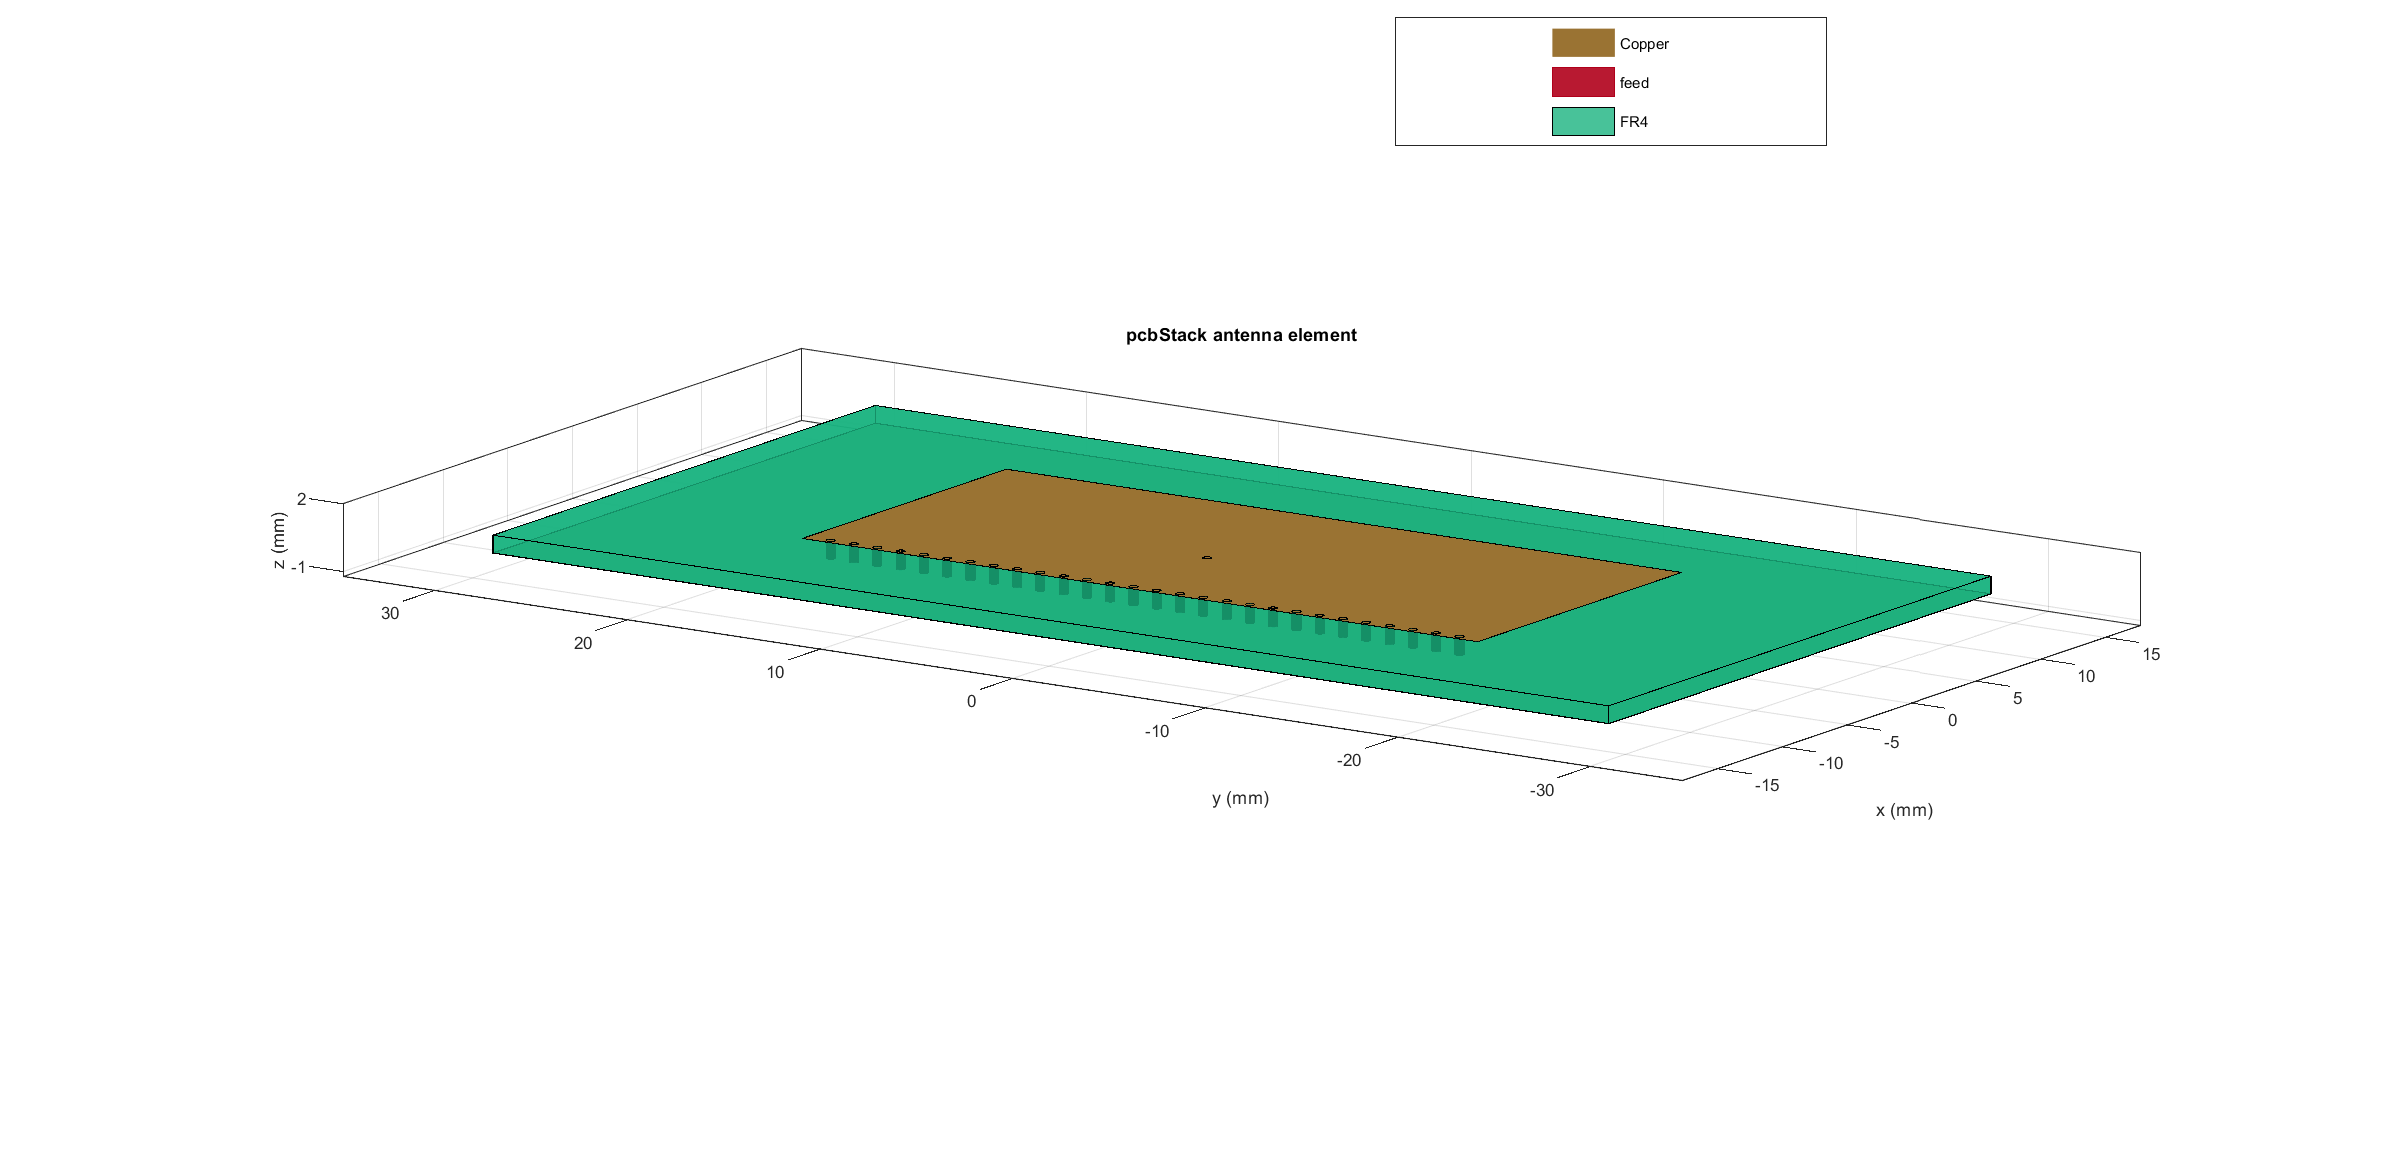
\includegraphics[scale=0.2]{pcb_shorting_pins_3d_view.pdf}
			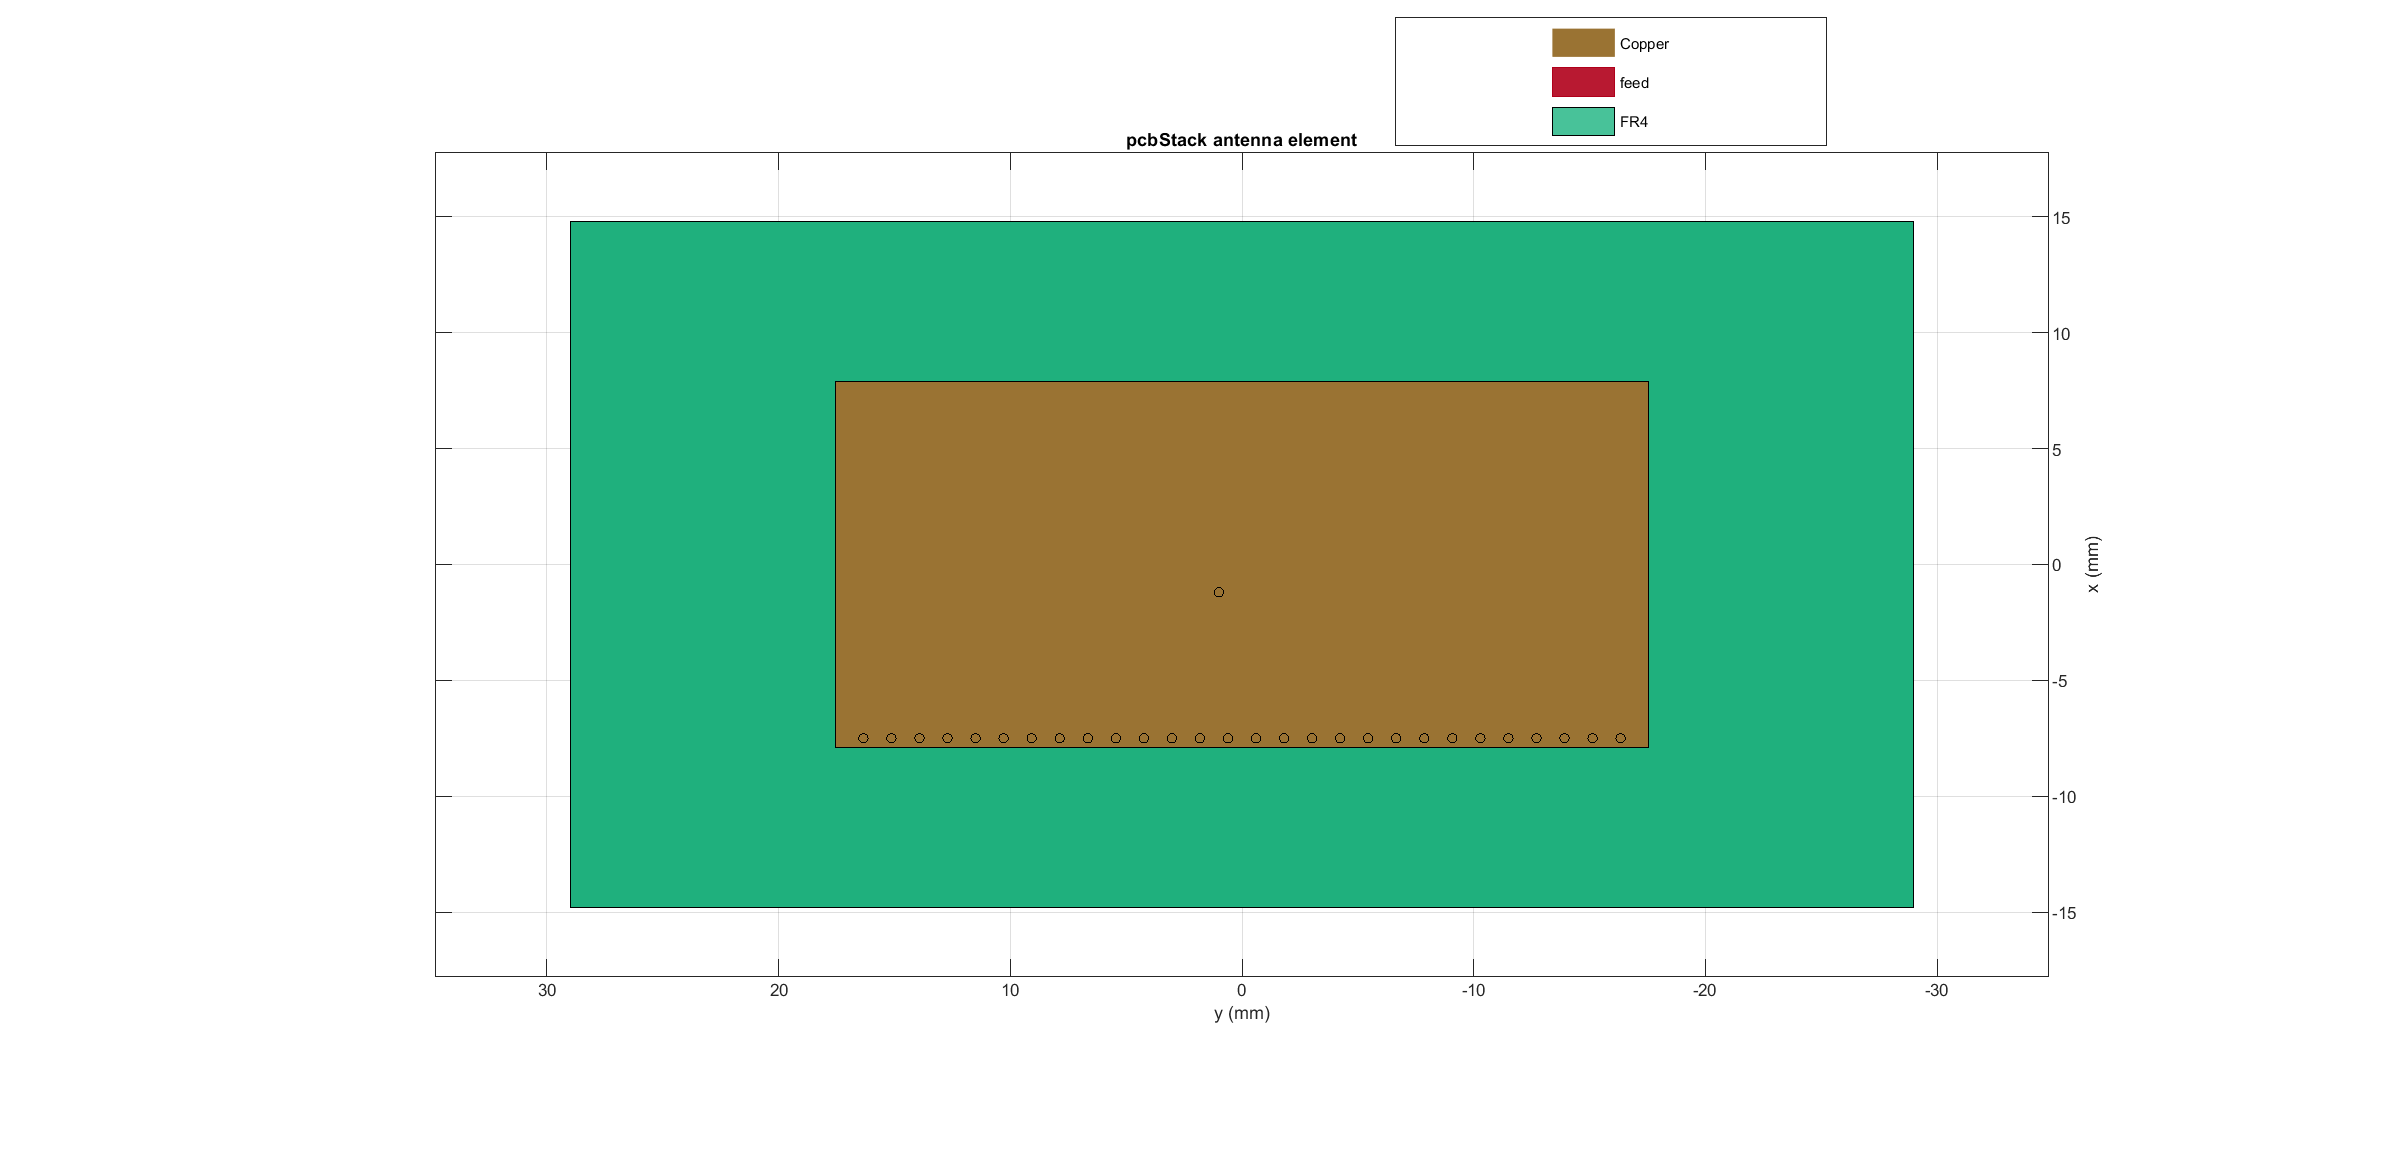
\includegraphics[scale=0.2]{pcb_shorting_pins_top_view.pdf}
		\caption{3D view and top view of the PIFA approximation realized with a PCB stack and cylindrical shorting pins}
		\label{fig:pcb shorting}
	\end{figure}
\end{center}
\begin{figure}[h]
	\begin{center}
		\begin{subfigure}{0.5\linewidth}
			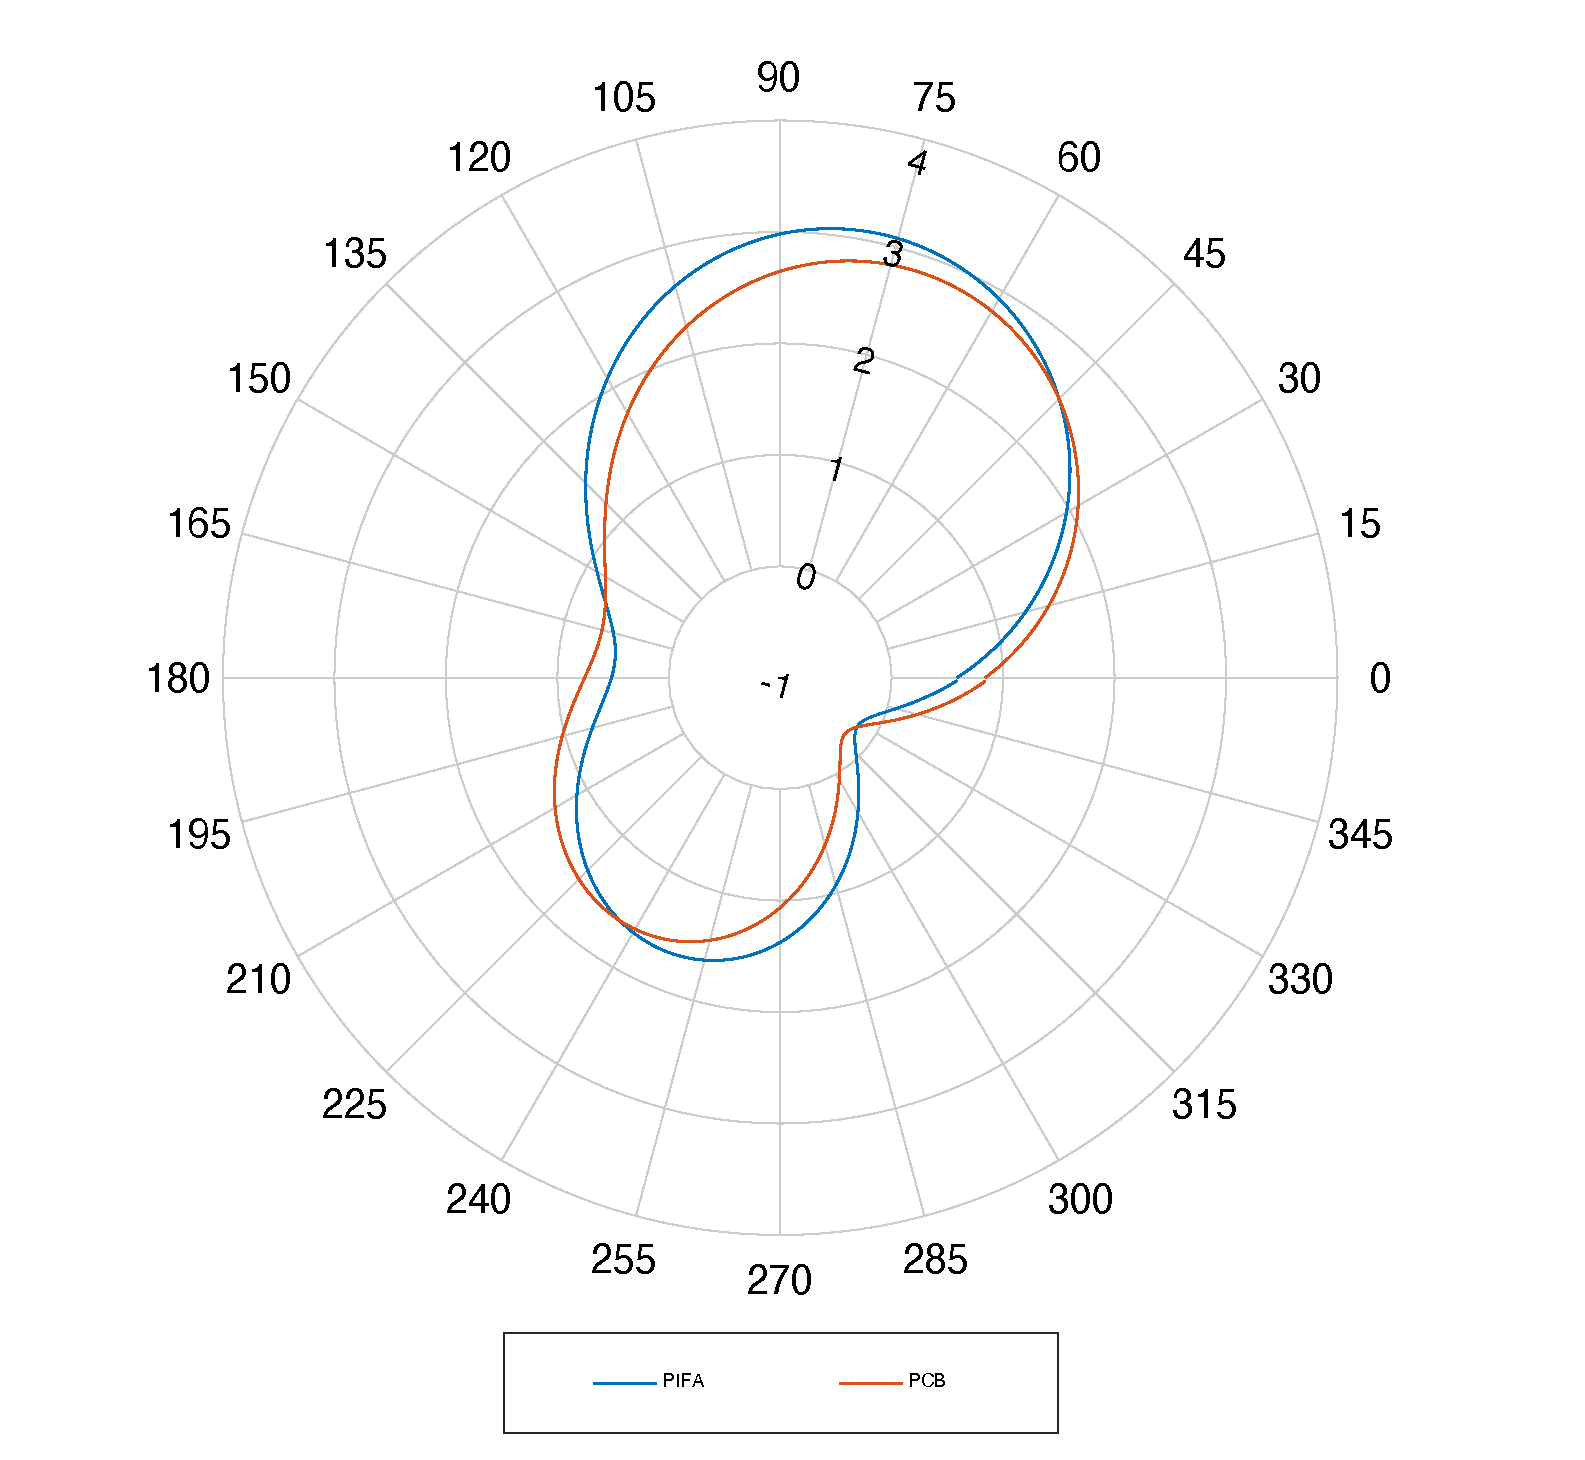
\includegraphics[scale=0.3]{pifa_pcb_null_azymuth_comparison.pdf}
			\caption{}
		\end{subfigure}
		\begin{subfigure}{0.5\linewidth}
			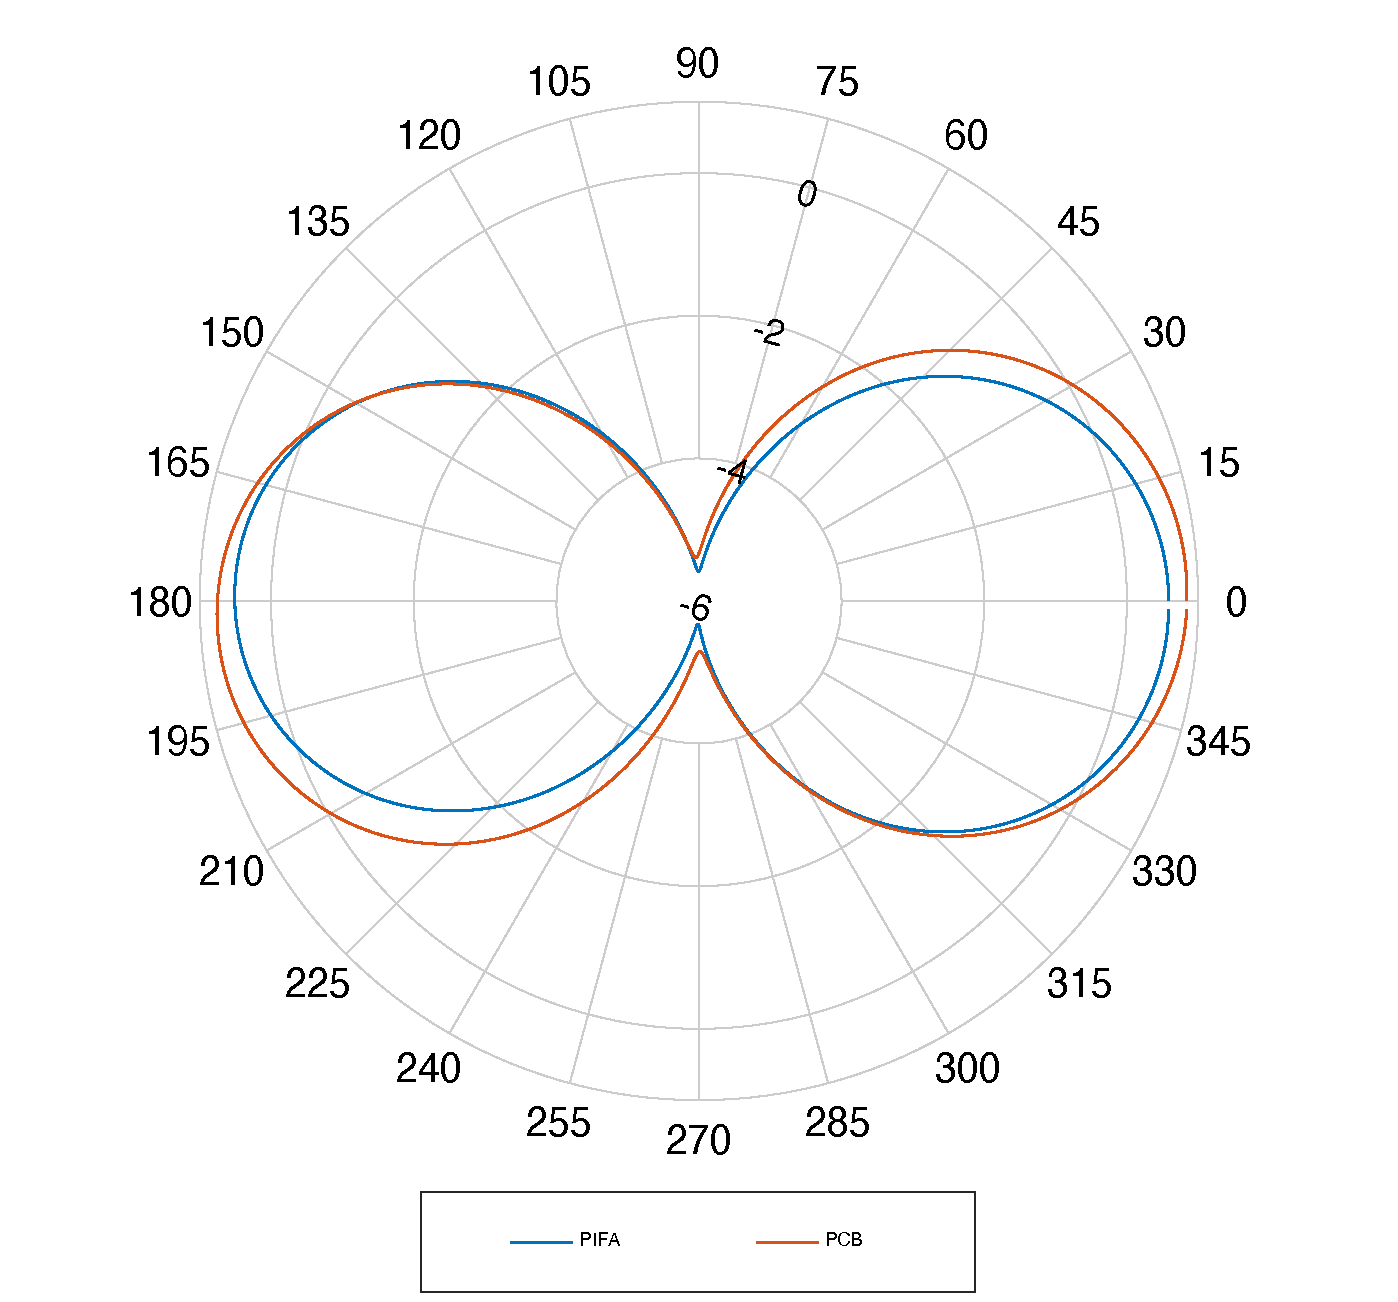
\includegraphics[scale=0.3]{pifa_pcb_null_elevation_comparison.pdf}
			\caption{}	\end{subfigure}
		\caption{
			PIFA and PCB single antenna directivity patterns (dB) in the Azimuth cut  ($\theta_{el}=0^\circ$, (a)) and in the Elevation cut ($\phi_{az}=0^\circ$, (b))}
	\end{center}  
\end{figure}
\begin{figure}[h]
	\begin{center}
		\begin{subfigure}{0.5\linewidth}
			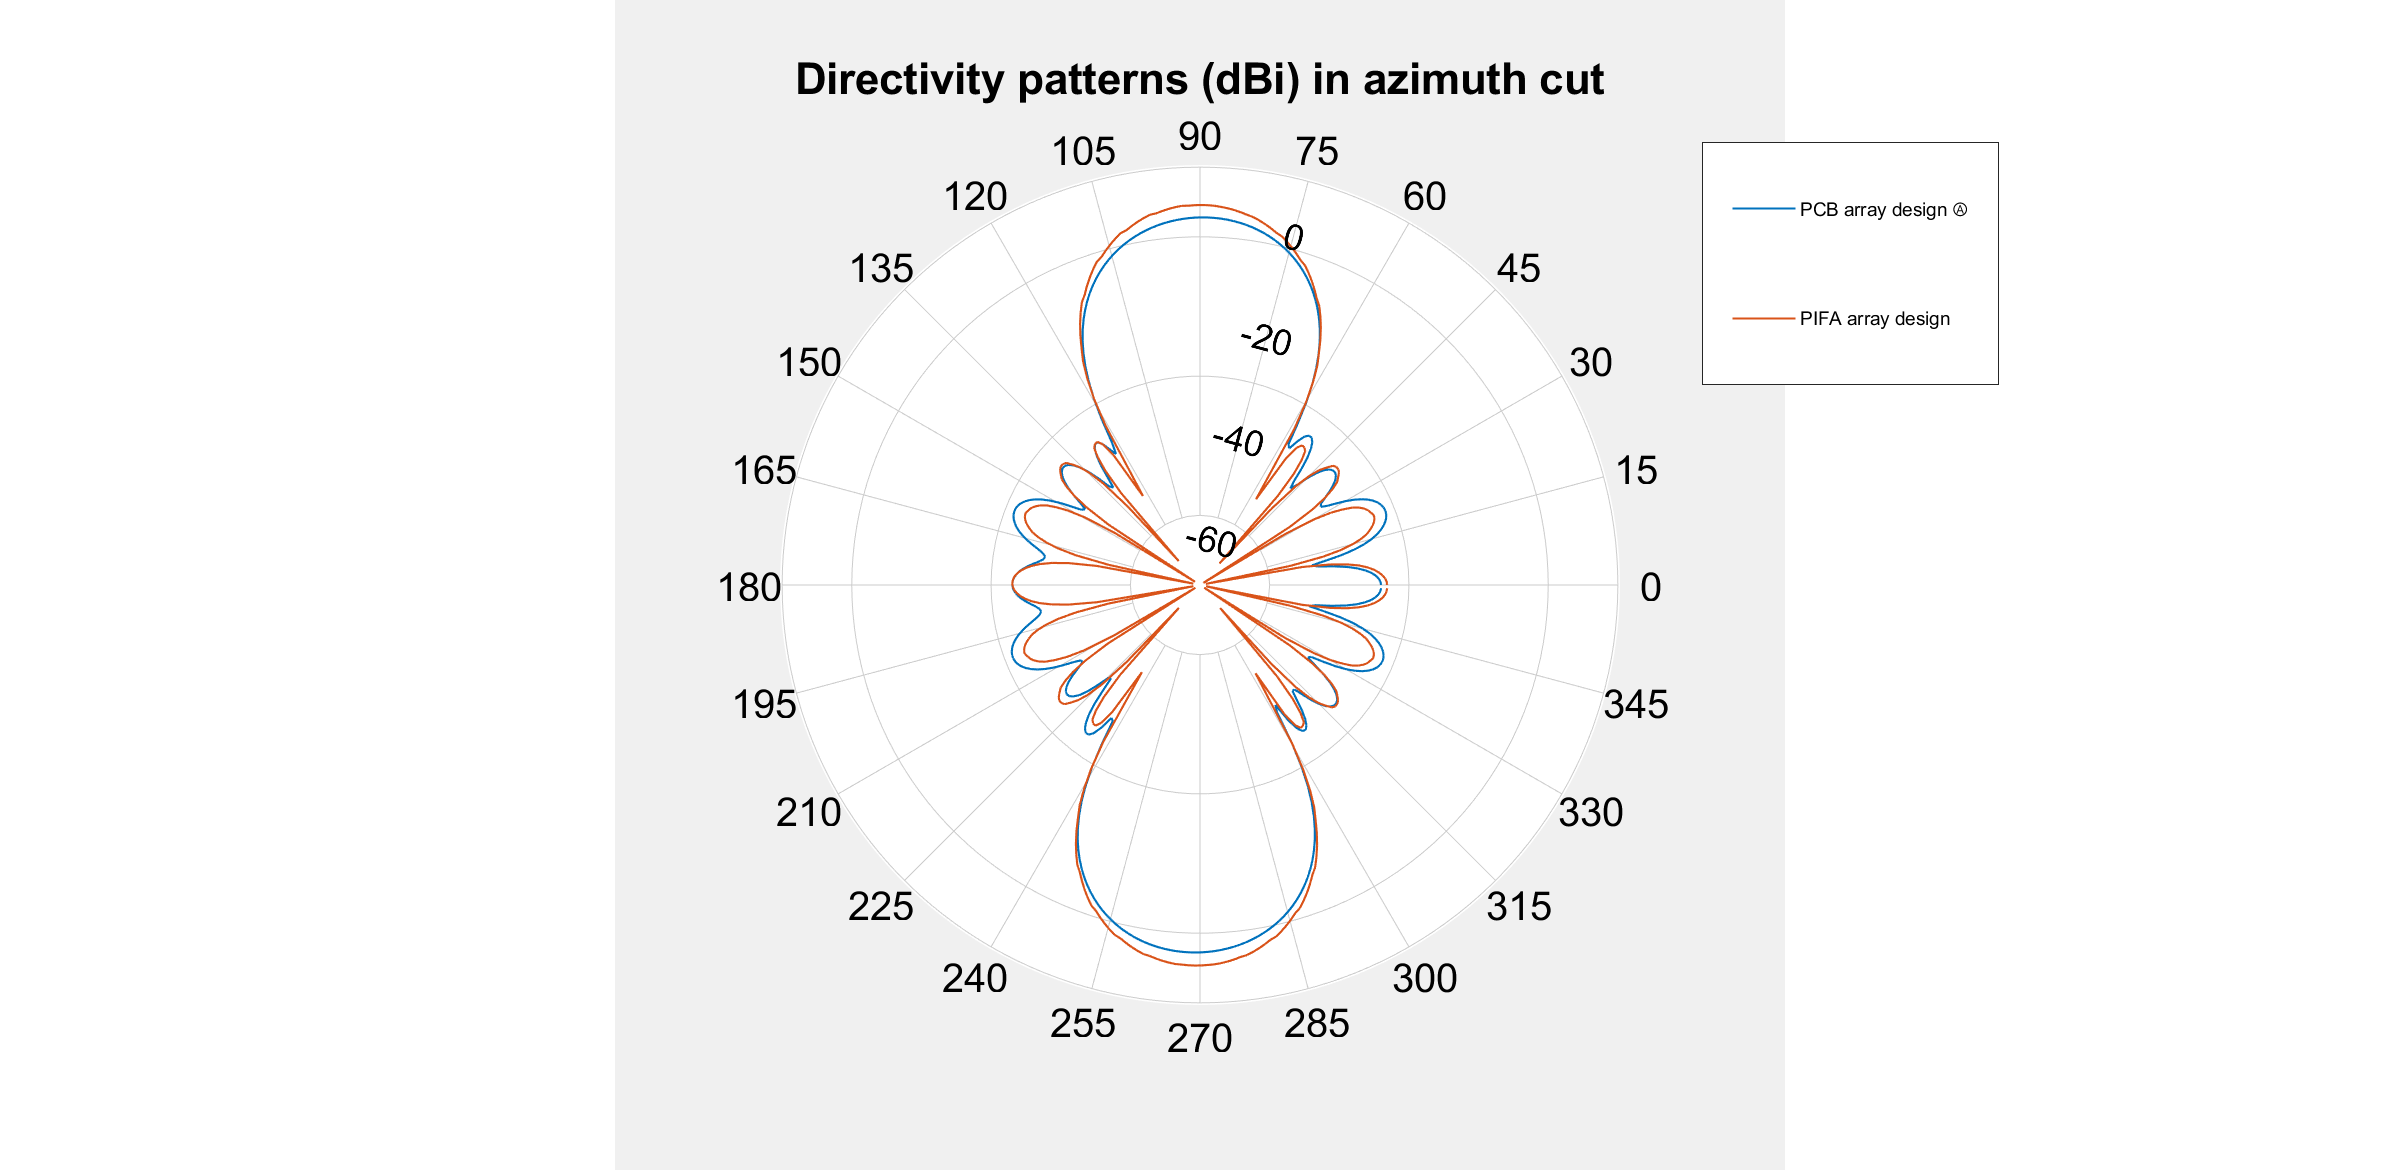
\includegraphics[scale=0.3]{pifa_pcb_array_azimuth_comparison.pdf}
			\caption{}
		\end{subfigure}
		\begin{subfigure}{0.5\linewidth}
			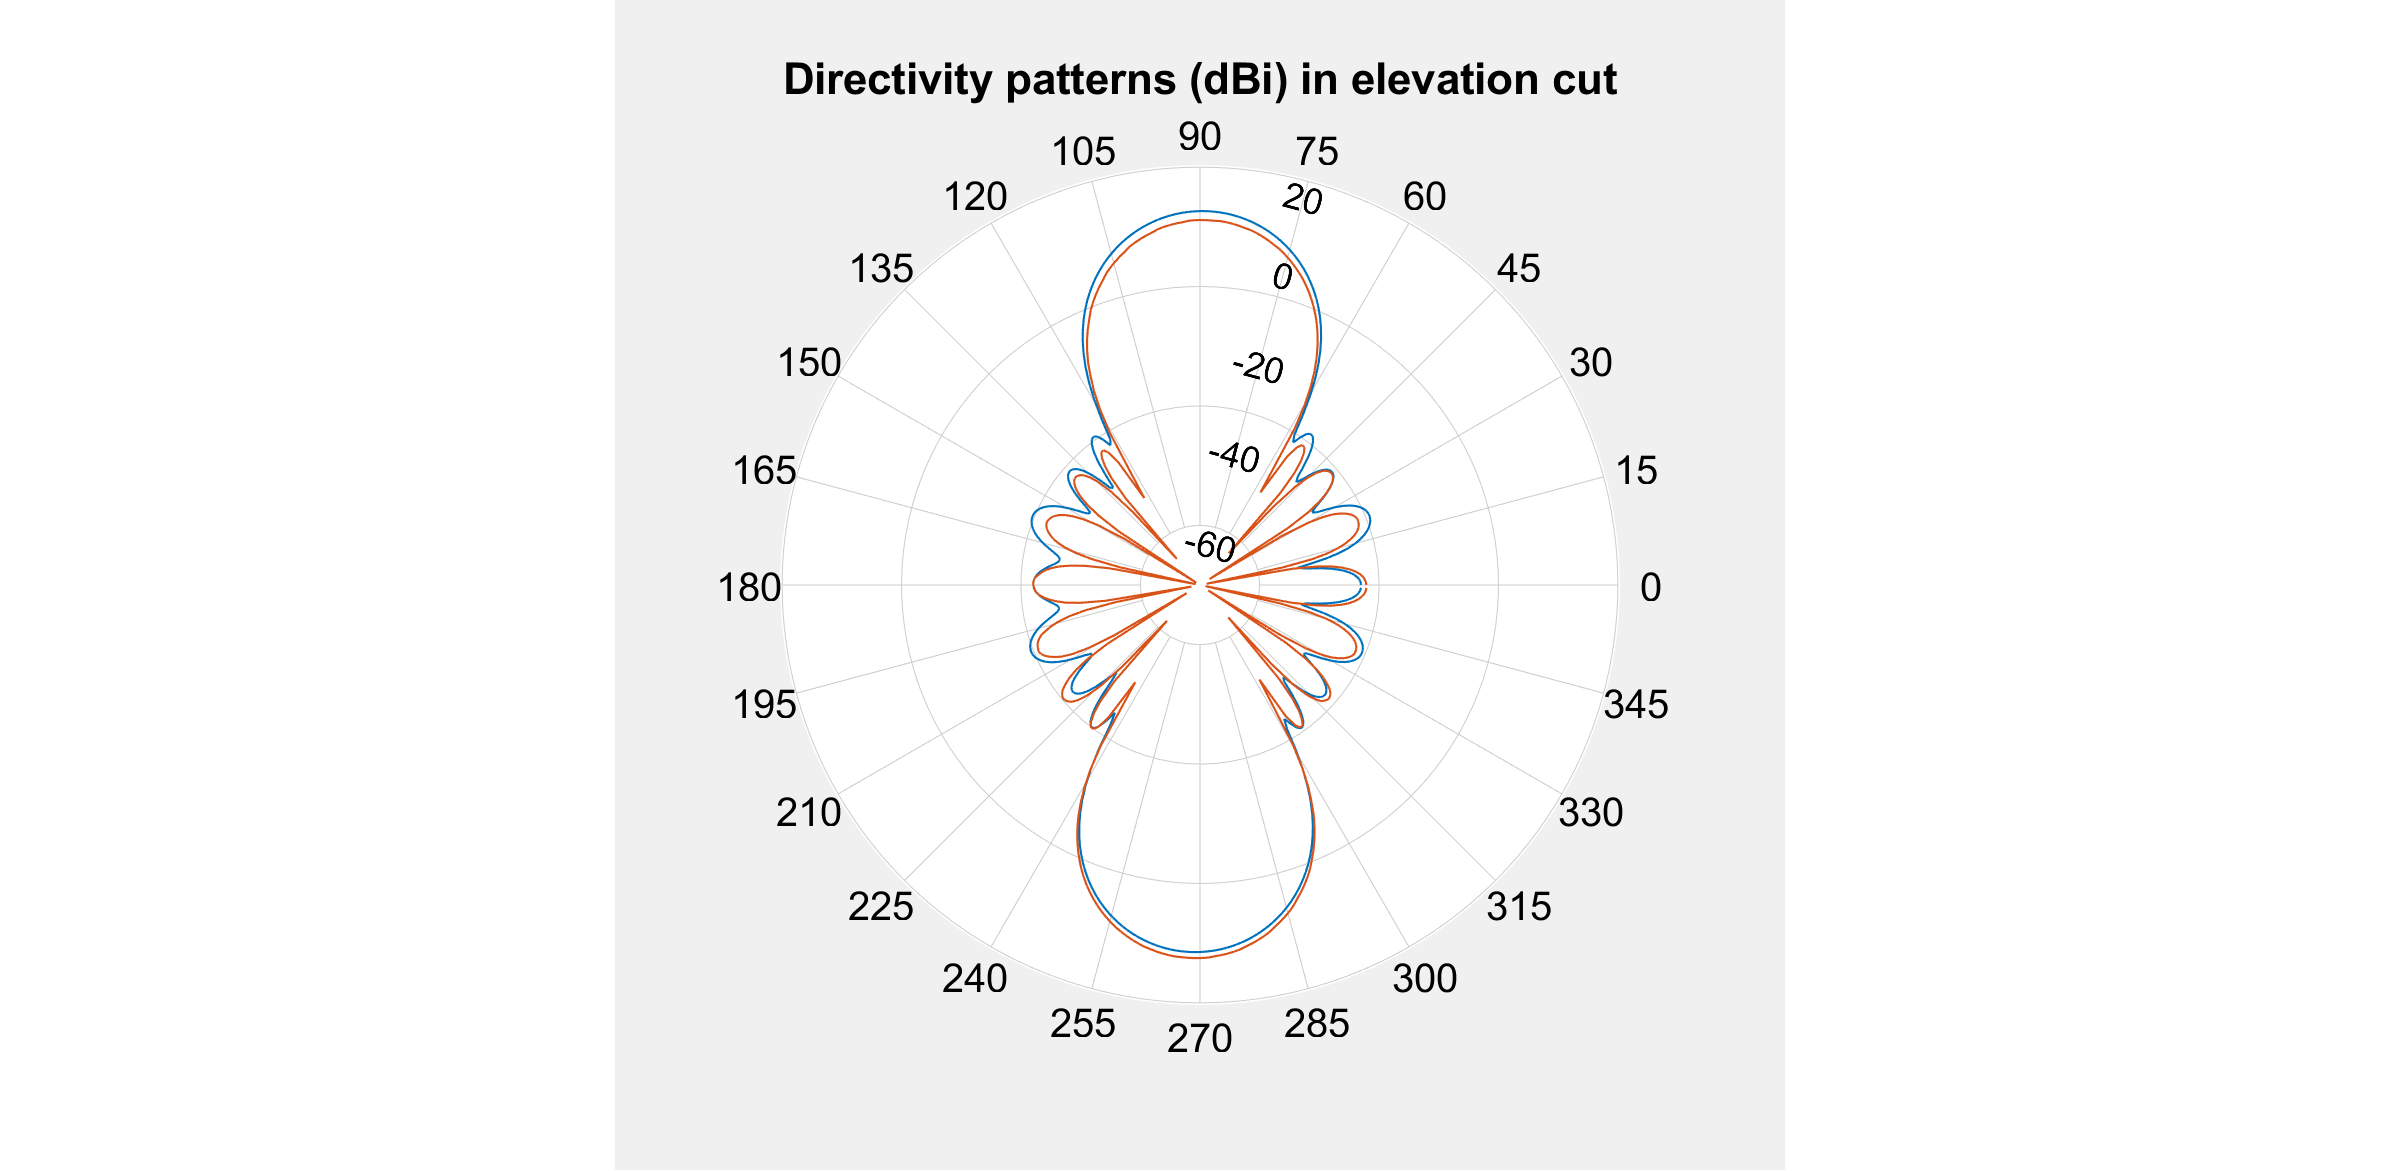
\includegraphics[scale=0.3]{pifa_pcb_array_elevation_comparison.pdf}
			\caption{}	\end{subfigure}
		\caption{
			PIFA and PCB arrays directivity patterns (dB) in the Azimuth cut  ($\theta_{el}=0^\circ$, (a)) and in the Elevation cut ($\phi_{az}=0^\circ$, (b))}
	\end{center}  
\end{figure}

\begin{center}
	\begin{figure}
		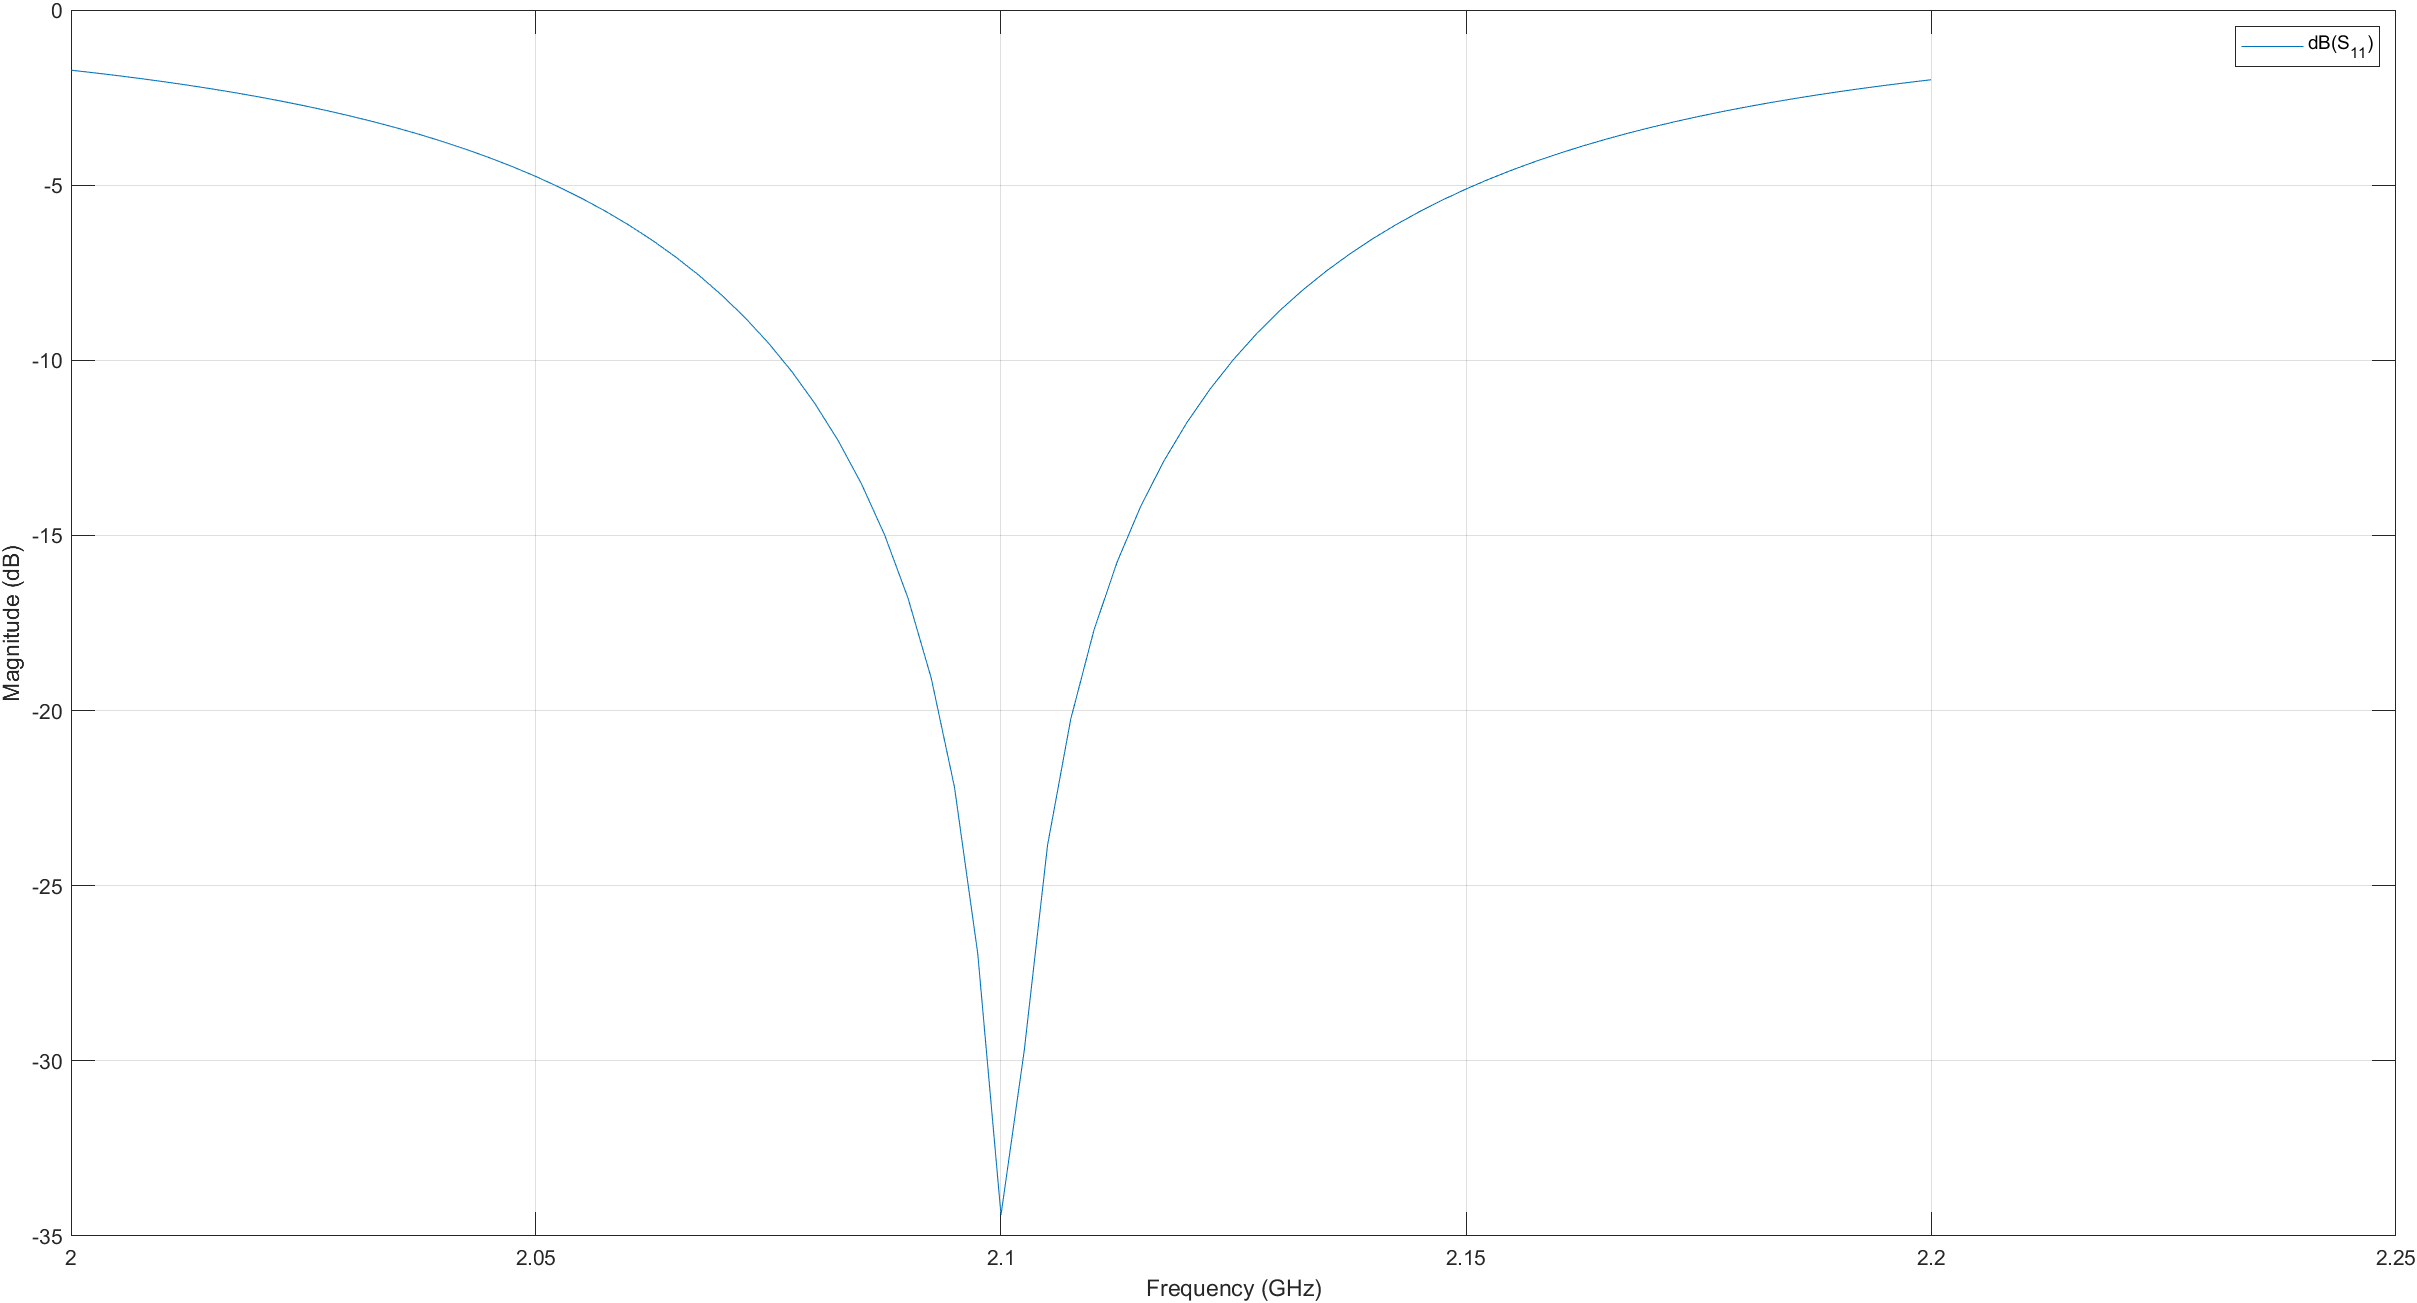
\includegraphics[width = 0.5\linewidth]{gamma.png}
		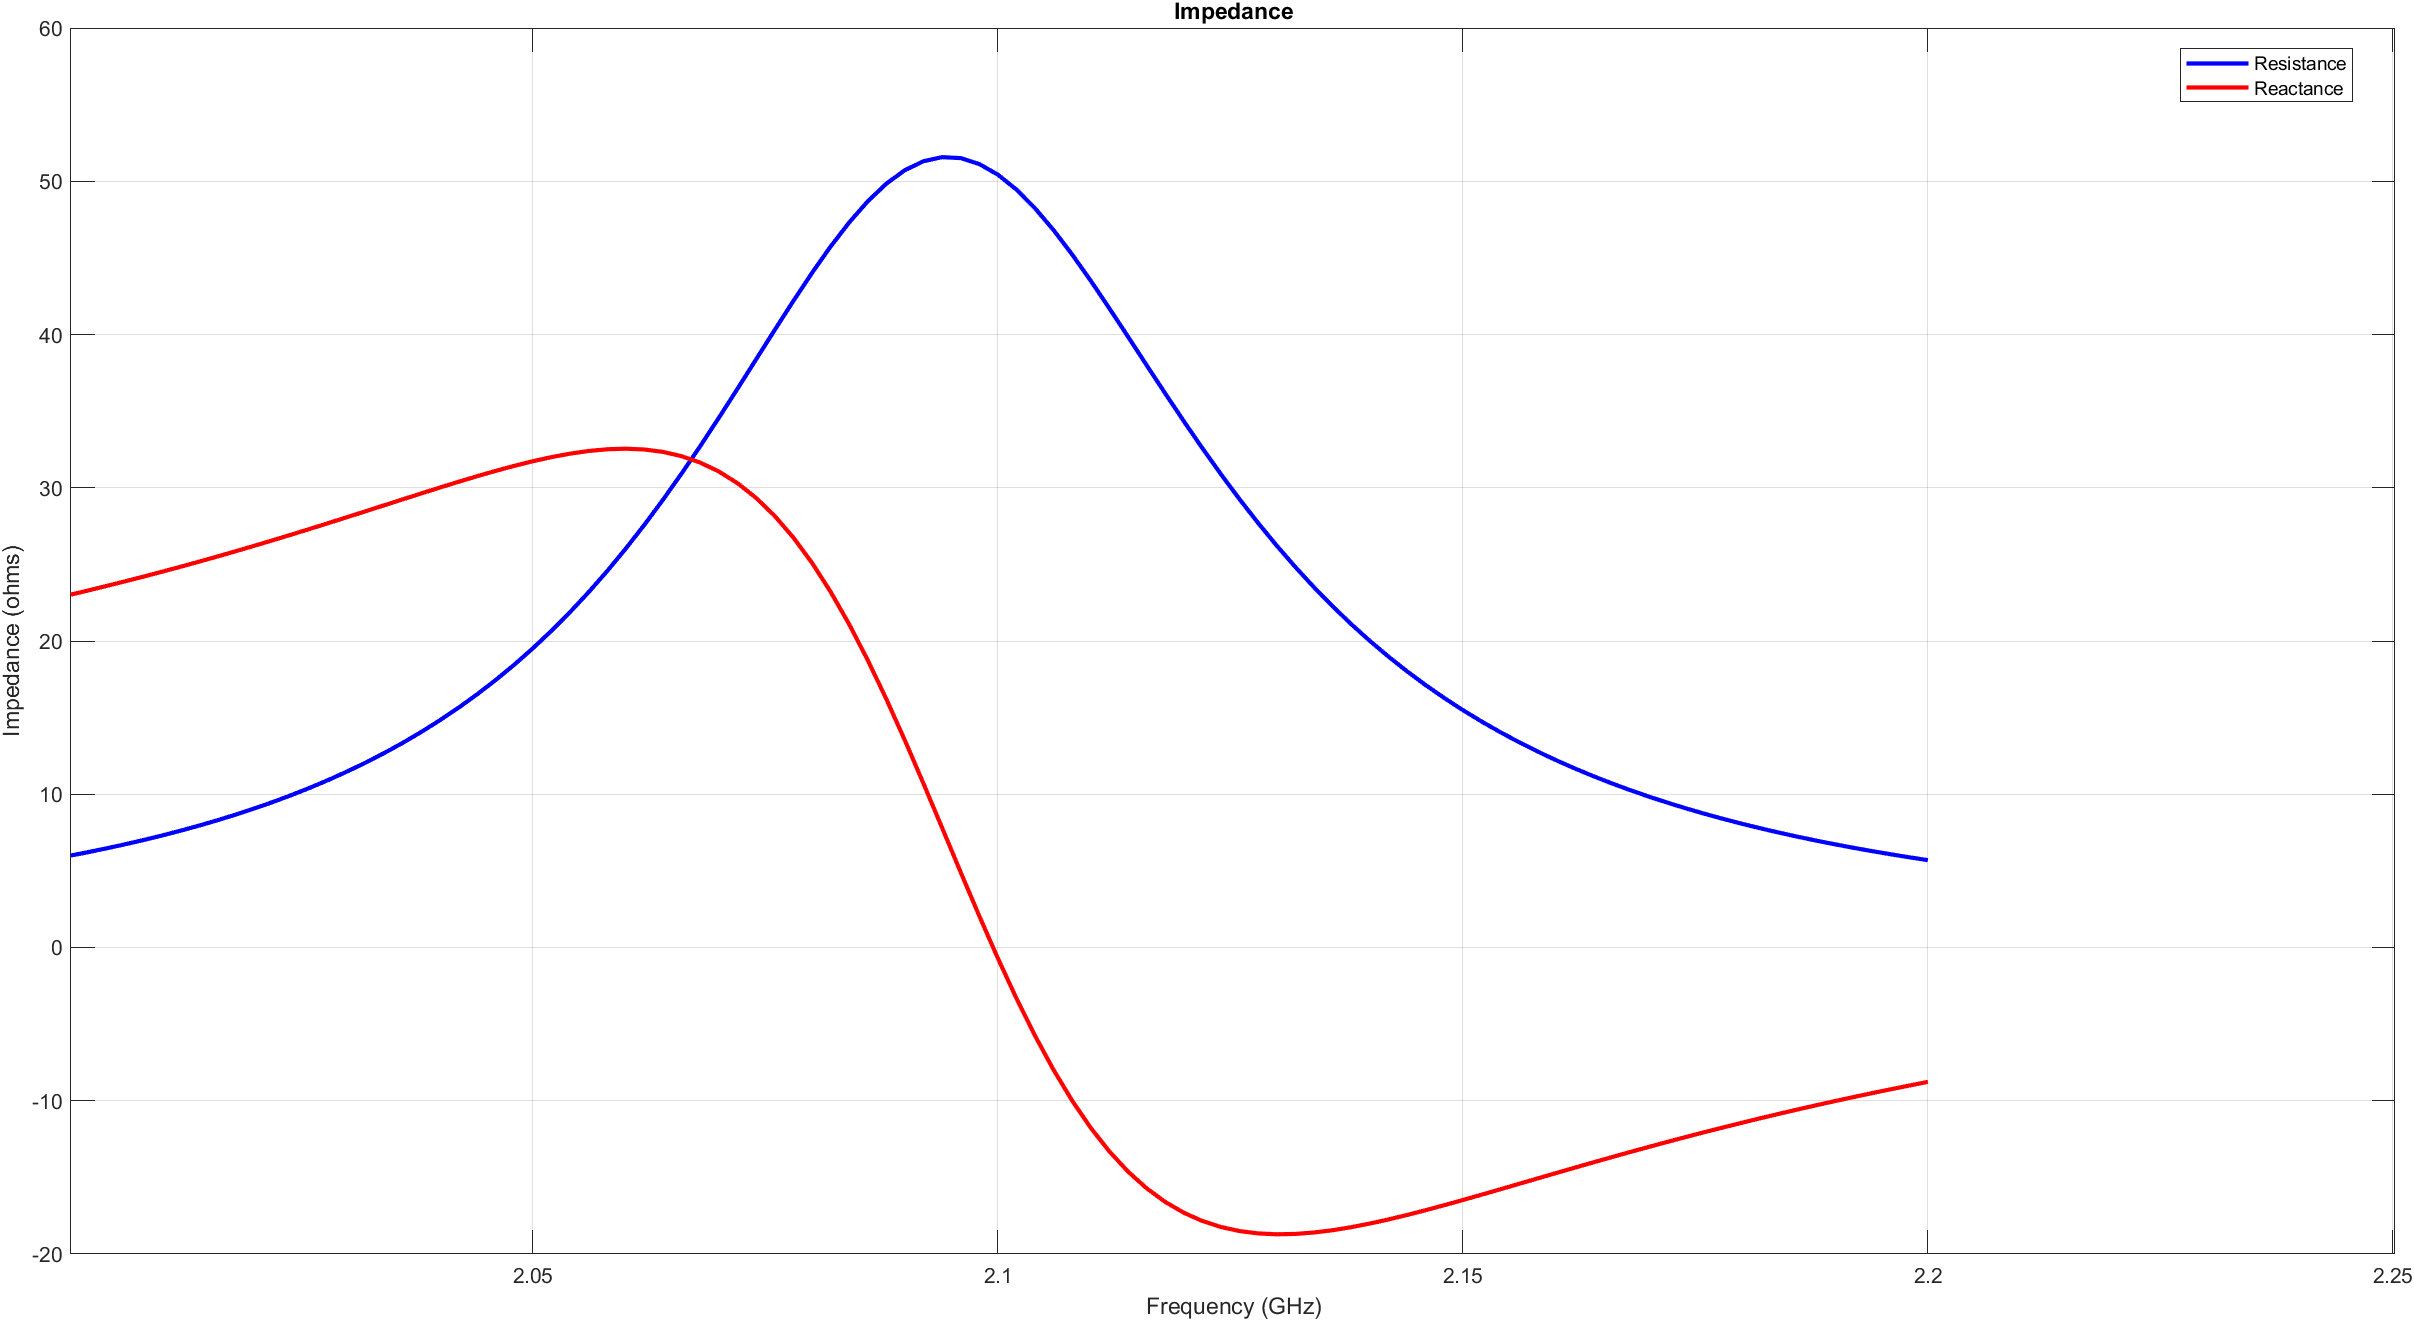
\includegraphics[width = 0.5\linewidth]{impedances.png}
		\caption{Reflection coefficient (left) and impedances (right) plots depending on $f\,\in\,2.0\div 2.1\,GHz$. This are the resulting plots before $W_{feed}$ optimization. }
	\end{figure}
\end{center}

\section*{\fontfamily{qag}\selectfont\color{Turquoise}Overall patch antenna array performance}
In this last part of the project, the array factor and the the element antenna (PIFA or PCB stack) designs will be combined so that their total effect will be examined. As it's been already mentioned in the previous paragraph, some of the information describing the overall array performance can be asked from both the \texttt{\color{Mahogany}Sensor Array Analyzer} (where the array of PIFAs was designed) and the \texttt{\color{Mahogany}PCB/Antenna Array Designer} (where the single patch antenna made starting from the PCB stack and also the whole array can be constructed). The performance of the overall array will be evaluated in two cases: in the broadside case ($90^\circ$) but also at $45^\circ$ off the boresight direction. First of all, it is very simple to identify the phase shift coefficients in the broadside case because they all equal $0^\circ$ (there's no actual phase shift between antennas). In the second case, some manual calculation can be made in order to insert the phase shifts between the single antennas (this is the case of the PCB stack array), and it can be also automatically computed by using the array of PIFAs. The generic procedure is shown in \textbf{\cref{eq:phase coefficients}}. Just before moving to the last part of the analysis, where only the characteristics of the array of PCBs will be considered, a last comparison between the array of PCBs and the array of PIFAs will be made in terms of 2D directivity patterns (both in broadside and in $45^\circ$ off the boreside direction, see \textbf{\cref{fig:pcb pifa array comparison}}). An error analysis based on the difference between the PCBs array main lobe and that of the PIFAs array, but also on the difference between the PCBs array main side lobe and that of the PIFAs array will be shown. The patterns and the numerical results according to the numerical error values illustrate how the array of PCBs represent a good enough approximation of the array of PIFAs. 
\subsection*{\fontfamily{qag}\selectfont\color{Turquoise}Total array gain}
In order to get and describe the last plots of the project, it is not possible to recur to the \texttt{\color{Mahogany}Sensor Array Analyzer} because some of the commands, such as  and \texttt{\color{Turquoise}EHfields} and \texttt{\color{Turquoise}patternMultiply}, are not available in this tool. Thus, in this last part, only the array of PCBs will be used, because it's compatible with these commands. The total array gain will be computed and displayed in two different cases: by means of a fullwave model (with no approximation) and by using the pattern multiplication principle. This second case is idealistic because it makes an approximation of the real patterns by not considering the mutual induced interactions between the single antennas of the array; however, a "mathematical" interaction is considered in this model because it comes out of a formulation that mixes the single element effect (which gives an element gain factor $G_0$) on the gain pattern with the angular filtering influence of the array factor, weighted by a combination of the current coefficients (which gives an array gain factor $G_F$). The overall idealistic case is based on the pattern multiplication principle, which (in a case such as the Tchebyshev array synthesis model, thus with non uniform amplitude feed), will take into account also the effect of the tapering efficiency ($\eta_T$) in its formulation (see \textbf{\cref{eq:pattern multiplication}}). Thus, the pattern multiplication principle can be applied angle by angle and this will provide a set of values that can be computed and inserted in matrices by using \texttt{\color{BurntOrange}MatLab}. Starting from the matrices, the 2D patterns can be represented. On the other hand, an easier way is to use the \texttt{\color{Turquoise}patternMultiply} command and get the ideal. 
\subsection*{\fontfamily{qag}\selectfont\color{Turquoise}Electric and magnetic near fields}
The near field characteristics (specifically those of the radiative field, also called the Fresnel region) have been analyzed in both the broadside and by beamsteering to $45^\circ$ off the boresight conditions. Two situations have been analyzed: the general near field behaviour (in its electric and magnetic field components) but also the specific orientation of the fields in the center position of each of the five elements composing the antenna (so considering the $x$ and $y$ coordinates of each patch corresponding to the length and width directions of its planar development and the $z$ coordinate corresponding to the verical Fresnel distance component from the origin in a global reference). 

\begin{figure}
	\begin{center}
		\begin{subfigure}{0.25\linewidth}
			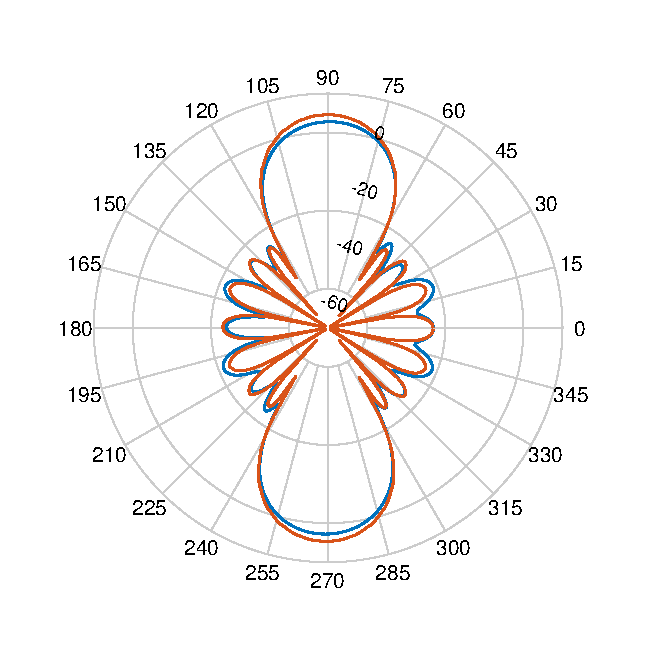
\includegraphics[scale=0.5]{pcb_pifa_array_azimuth_90_comparison.pdf}
			\caption{}
		\end{subfigure}
		\begin{subfigure}{0.25\linewidth}
		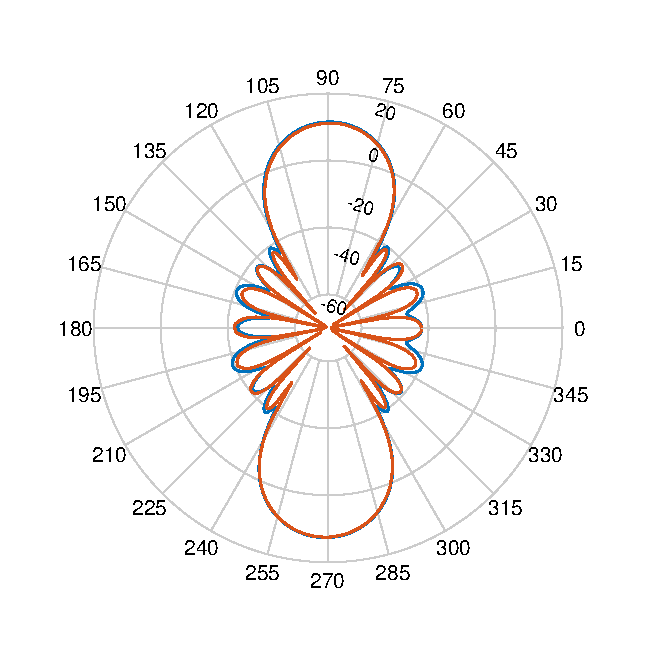
\includegraphics[scale=0.5]{pcb_pifa_array_elevation_90_comparison.pdf}
		\caption{}
	\end{subfigure}

		\begin{subfigure}{0.25\linewidth}
	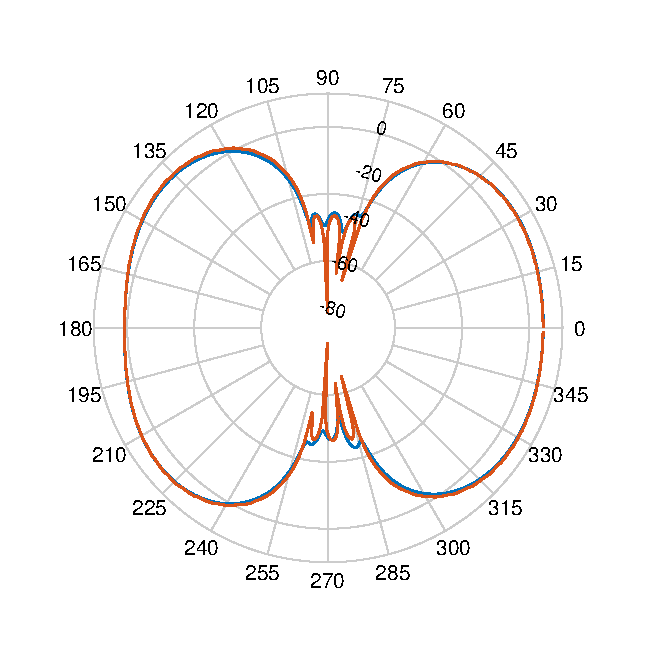
\includegraphics[scale=0.5]{pcb_pifa_array_azimuth_45_comparison.pdf}
	\caption{}
\end{subfigure}
\begin{subfigure}{0.25\linewidth}
	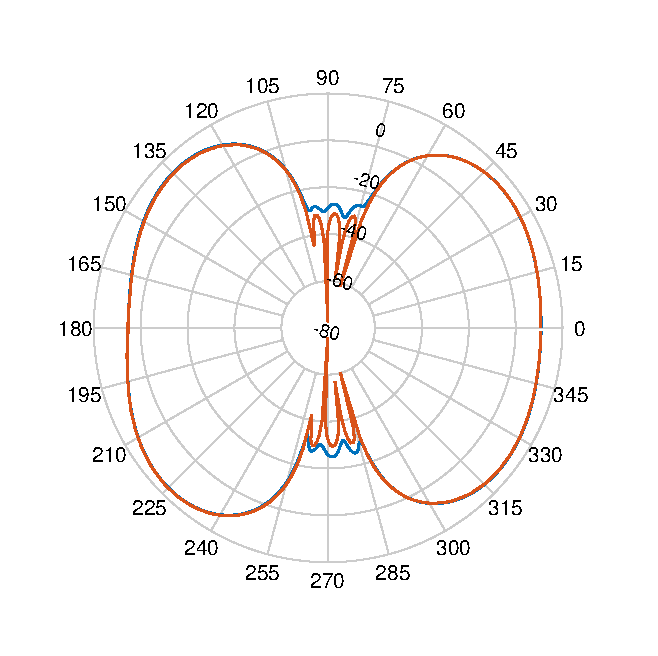
\includegraphics[scale=0.5]{pcb_pifa_array_elevation_45_comparison.pdf}
	\caption{}
\end{subfigure}
\caption{2D patterns in both the broadside case ((a) azimuth cut and (b) elevation cut) and $45^\circ$ off the boresight direction ((c) azimuth cut and (d) elevation cut).}
\label{fig:pcb pifa array comparison}
	\end{center}
\end{figure}
\begin{equation}
	\begin{aligned}
		u_0&=\alpha d_{opt}\,=\,2\pi\frac{d_{opt}}{\lambda}\,\cos(\theta_0)\\
		\alpha_n&=n\,\alpha\,d_{opt}=nu_0\qquad \left(n=\overline{1,5}\right)
		\label{eq:phase coefficients}
	\end{aligned}
\end{equation}

\begin{equation}
	G_{total}=\,\eta_T\,G_0\,G_T
	\label{eq:pattern multiplication}
\end{equation}




\newpage 
%\section*{References}

\printbibliography

}

\end{document}